% Document de classe yathesis, en 12 points, interligne un et demi, et version finale
\documentclass[11pt,space=onehalf,version=submitted]{yathesis}
%
% Chargement manuel de packages (pas déjà chargés par la classe yathesis)
\usepackage[T1]{fontenc}
\usepackage[utf8]{inputenc}
\usepackage{svg}
% \usepackage{lipsum} % À proscrire dans un vrai mémoire de thèse !\
\usepackage{amsthm}
\usepackage{kpfonts}
\usepackage{algorithm2e}
\usepackage{booktabs}
\usepackage{siunitx}
\usepackage{pgfplots}
\usepackage{caption}
\usepackage{subcaption}
\usepackage{listings}
\usepackage{xcolor}
\usepackage{tcolorbox}
\usepackage{microtype}
% \usepackage[american]{babel}

% Code styling
\definecolor{codegreen}{rgb}{0,0.6,0}
\definecolor{codegray}{rgb}{0.5,0.5,0.5}
\definecolor{codepurple}{rgb}{0.58,0,0.82}
\definecolor{backcolour}{rgb}{0.95,0.95,0.92}

\lstdefinestyle{mystyle}{
    backgroundcolor=\color{backcolour},   
    commentstyle=\color{codegreen},
    keywordstyle=\color{magenta},
    numberstyle=\color{codegray},
    stringstyle=\color{codepurple},
    basicstyle=\ttfamily\tiny,
    breakatwhitespace=false,         
    breaklines=True,                 
    captionpos=b,                    
    keepspaces=true,                 
    numbers=none,                    
    showspaces=false,                
    showstringspaces=false,
    showtabs=false,                  
    tabsize=2
}

\lstset{style=mystyle}
\usepackage{varioref}
\usepackage[xindy,quiet]{imakeidx}
\usepackage[autostyle]{csquotes}
\usepackage[backend=biber,safeinputenc]{biblatex}
\usepackage{hyperref}
\usepackage[xindy,acronyms,symbols]{glossaries}
%

\newtheorem{definition}{Definition}
\newtheorem{proposition}{Proposition}
\newtheorem{theorem}{Theorem}
\newtheorem{lemma}{Lemma}


% Génération de l'index
\makeindex
%
% Spécification de la ou des ressources bibliographiques
\addbibresource{auxiliaires/bibliographie.bib}
\addbibresource{biblatex-examples.bib} % Fournie par biblatex.
%
% Génération du glossaire
\makeglossaries
%
% (Facultatif) Configuration des styles du glossaire et de la liste d'acronymes
% (à n'utiliser que si le package « glossaries » est chargé)
% \setglossarystyle{indexhypergroup}
% \setacronymstyle{long-sc-short}
%
% (Facultatif) Spécification de la ou des ressources terminologiques
% \loadglsentries{auxiliaires/glossaire}
% \loadglsentries{auxiliaires/acronymes}
% \loadglsentries{auxiliaires/symboles}
%
% Les réglages figurant habituellement dans le préambule, notamment concernant
% la bibliographie et l'éventuel index, peuvent être saisis dans le fichier
% « thesis.cfg » (situé dans le sous-dossier « configuration ») qui est
% automatiquement importé par la classe yathesis.
%
% Importation manuelle du fichier de macros personnelles
% \input{configuration/macros}
%
% Commande permettant de faire figurer d'un seul coup toutes les références des
% ressources bibliographiques ci-dessus, même si elles ne sont pas citées
% explicitement (à proscrire dans un vrai mémoire de thèse !)
%
%%%%%%%%%%%%%%%%%%%%%%%%%%%%%%%%%%%%%%%%%%%%%%%%%%%%%%%%%%%%%%%%%%%%%%%%%%%%%%%
%%%%%%%%%%%%%%%%%%%%%%%%%%%%%%%%%%%%%%%%%%%%%%%%%%%%%%%%%%%%%%%%%%%%%%%%%%%%%%%
% Début du document
%%%%%%%%%%%%%%%%%%%%%%%%%%%%%%%%%%%%%%%%%%%%%%%%%%%%%%%%%%%%%%%%%%%%%%%%%%%%%%%
%%%%%%%%%%%%%%%%%%%%%%%%%%%%%%%%%%%%%%%%%%%%%%%%%%%%%%%%%%%%%%%%%%%%%%%%%%%%%%%
\begin{document}
%
%%%%%%%%%%%%%%%%%%%%%%%%%%%%%%%%%%%%%%%%%%%%%%%%%%%%%%%%%%%%%%%%%%%%%%%%%%%%%%%
% Caractéristiques du document
%%%%%%%%%%%%%%%%%%%%%%%%%%%%%%%%%%%%%%%%%%%%%%%%%%%%%%%%%%%%%%%%%%%%%%%%%%%%%%%
%
% Préparation des pages de couverture et de titre
%%%%%%%%%%%%%%%%%%%%%%%%%%%%%%%%%%%%%%%%%%%%%%%%%%%%%%%%%%%%%%%%%%%%%%%%%%%%%%%
% Les caractéristiques de la thèse sont saisies dans le fichier
% « characteristics.tex » (situé dans le dossier « configuration »).
%
% Production des pages de couverture et de titre
%%%%%%%%%%%%%%%%%%%%%%%%%%%%%%%%%%%%%%%%%%%%%%%%%%%%%%%%%%%%%%%%%%%%%%%%%%%%%%%
\maketitle
%
%%%%%%%%%%%%%%%%%%%%%%%%%%%%%%%%%%%%%%%%%%%%%%%%%%%%%%%%%%%%%%%%%%%%%%%%%%%%%%%
% Début de la partie liminaire de la thèse
%%%%%%%%%%%%%%%%%%%%%%%%%%%%%%%%%%%%%%%%%%%%%%%%%%%%%%%%%%%%%%%%%%%%%%%%%%%%%%%
%
% (Facultatif) Production de la page de clause de non-responsabilité
% \makedisclaimer
%
% (Facultatif) Production de la page de mots clés
% \makekeywords
%
% (Facultatif) Production de la page affichant les logo, nom et coordonnées du
% ou des laboratoires (ou unités de recherche) où la thèse a été préparée
% \makelaboratory
%
% (Facultatif) Dédicace(s)
% \input{liminaires/dedicaces}
%
% (Facultatif) Épigraphe(s)
% \input{liminaires/epigraphes}
%
% Résumés succincts
% Résumés (de 1700 caractères maximum, espaces compris) dans la
% langue principale (1re occurrence de l'environnement « abstract »)
% et, facultativement, dans la langue secondaire (2e occurrence de
% l'environnement « abstract »)
\begin{abstract}
  Dans cette thèse de doctorat, nous étudions des algorithmes d'apprentissage d'arbres de décision pour la classification et la prise de décision séquentielle. Les arbres de décision sont interprétables car les humains peuvent lire les opérations de l'arbre de décision depuis la racine jusqu'aux feuilles. Cela fait des arbres de décision le modèle de référence lorsque la vérification humaine est requise, comme dans les applications médicales. Cependant, les arbres de décision ne sont pas différentiables, ce qui les rend difficiles à optimiser, contrairement aux réseaux neuronaux qui peuvent être entraînés efficacement avec la descente de gradient. Les approches existantes d'apprentissage par renforcement interprétables apprennent généralement des arbres souples (non interprétables en l'état) ou sont ad hoc (entraînent un réseau neuronal puis entraînent un arbre à imiter le réseau). Cet apprentissage d'arbre indirect ne garantit pas de trouver des bonnes solutions pour le problème initial.

  Dans la première partie de ce manuscrit, nous visons à apprendre directement des arbres de décision pour un processus de décision Markovien avec de l'apprentissage par renforcement. En pratique, nous montrons que cela revient à résoudre un problème de décision Markovien partiellement observable (PDMPO). La plupart des algorithmes d'apprentissage par renforcement existants ne sont pas adaptés aux PDMPOs. Ce parallèle entre l'apprentissage des arbres de décision et la résolution des PDMPOs nous aide à comprendre pourquoi, dans la pratique, il est souvent plus facile d'obtenir une politique experte non interprétable (un réseau neuronal) puis de la distiller en un arbre plutôt que d'apprendre l'arbre de décision à partir de zéro.

  La deuxième contribution de ce travail découle de l'observation selon laquelle la recherche d'un classifieur (ou régresseur) arbre de décision est une instance complètement observable du problème précédent. Nous formulons donc l'induction d'arbres de décision comme la résolution d'un problème de décision Markovien et proposons un nouvel algorithme de pointe qui peut être entraîné à partir de données d'exemple supervisés et qui généralise bien à des données nouvelles.

  Les travaux des parties précédentes reposent sur l'hypothèse que les arbres de décision sont un modèle interprétable que les humains peuvent utiliser dans des applications sensibles. Mais est-ce vraiment le cas ? Dans la dernière partie de cette thèse, nous tentons de répondre à des questions plus générales sur l'interprétabilité : pouvons-nous mesurer l'interprétabilité sans intervention humaine ? Et les arbres de décision sont-ils vraiment plus interprétables que les réseaux neuronaux ?

\end{abstract}
\begin{abstract}
  In this Ph.D. thesis, we study algorithms to learn decision trees for classification and sequential decision-making. Decision trees are interpretable because humans can read through the decision tree computations from the root to the leaves. This makes decision trees the go-to model when human verification is required like in medicine applications. However, decision trees are non-differentiable making them hard to optimize unlike neural networks that can be trained efficiently with gradient descent. Existing interpretable reinforcement learning (RL) approaches usually learn soft trees (non-interpretable as is) or are ad-hoc (train a neural network then fit a tree to it) potentially missing better solutions.

  In the first part of this manuscript, we aim to directly learn decision trees for a Markov decision process with reinforcement learning. In practice we show that this amounts to solving a partially observable Markov decision problem (POMDP). Most existing RL algorithms are not suited for POMDPs. This parallel between decision tree learning with RL and POMDPs solving help us understand why in practice it is often easier to obtain a non-interpretable expert policy--a neural network--and then distillate it into a tree rather than learning the decision tree from scratch.

  The second contribution from this work arose from the observation that looking for a decision tree classifier (or regressor) is a fully observable instance of the above problem. We thus formulate decision tree induction as solving a Markov decision problem and propose a new state-of-the-art algorithm that can be trained with supervised example data and generalizes well to unseen data.

  Work from the previous parts rely on the hypothesis that decision trees are indeed an interpretable model that humans can use in sensitive applications. But is it really the case? In the last part of this thesis, we attempt to answer some more general questions about interpretability: can we measure interpretability without humans? And are decision trees really more interpretable than neural networks?
\end{abstract}
%
% Production de la page de résumés
\makeabstract{}


%
% (Facultatif) Chapitre de remerciements
% \chapter{Remerciements}
I would like to thank my advisors Riad and Philippe for making my PhD the most rewarding three years of my life.
I would like to thank my old and new friends for making those three years fun.
I would like to thank my partner Alëna for being so supportive and loving.
I would like to thank my family for encouraging me to pursue such an interesting career.
I would also like to thank all the teachers I got since I was a kid for transmitting their passion for science.
I would like to thank all the Inria staff for making our work environment functional.

Have fun reading this manuscript.

%
% (Facultatif) Chapitre d'avertissement
% \include{liminaires/avertissement}
%
% (Facultatif) Liste des acronymes
% \printacronyms
%
% (Facultatif) Liste des symboles
% \printsymbols
%
% (Facultatif) Chapitre d'avant-propos
% \include{liminaires/avant-propos}
%
% Sommaire
\tableofcontents
%
% (Facultatif) Liste des tableaux
% \listoftables
%
% (Facultatif) Table des figures
% \listoffigures
%
% (Facultatif) Table des listings (nécessite que le package « listings » soit
% chargé)
% \lstlistoflistings
%
%%%%%%%%%%%%%%%%%%%%%%%%%%%%%%%%%%%%%%%%%%%%%%%%%%%%%%%%%%%%%%%%%%%%%%%%%%%%%%%
% Début de la partie principale (du « corps ») de la thèse
%%%%%%%%%%%%%%%%%%%%%%%%%%%%%%%%%%%%%%%%%%%%%%%%%%%%%%%%%%%%%%%%%%%%%%%%%%%%%%%
\mainmatter
%
% Chapitre d'introduction (générale)
%%%%%%%%%%%%%%%%%%%%%%%%%%%%%%%%%%%%%%%%%%%%%%%%%%%%%%%%%%%%%%%%%%%%%%%%%%%%%%%
\chapter*{Preliminary Concepts}

\section{What is Sequential Decision Making?}
In this manuscript we are interested in sequential decision making processes. Sequential decision making processes are found in all aspects of life. In medicine, {\color{blue}doctors} have to decide when {\color{orange}to use chimiotherapy} next based on {\color{green} the patient's current health} in order {\color{red}to heal} (cite). In agriculture, agronomists have to decide when to fertilize next based on the current soil and wheather conditions in order to maximize plant growth (cite). In automotive, the auto-pilot system has to decide how to steer the wheel next in order to maintain a safe trajectory (cite). In video games, a bot decides what attack to throw next based on the player's and its states in order to provide the best entertainment (cite).
Those sequential decision making processes exhibits key similarities: {\color{blue}an agent} takes {\color{orange}actions} based on {\color{green}some current information} to achieve some {\color{red}goal}. 

\subsection{Markov decision processes/problems}

\subsection{Exact solutions}

\subsection{Reinforcement learning}

\section{What is Interpretable Sequential Decision Making?}

\subsection{Why do we care about interpretability?}


\subsection{What are existing approaches for interpretable sequential decision making?}


\subsection{What are decision tree policies?}


\subsection{Why are decision tree policies harder to learn than decision tree classifiers?}

\section{Outline of the Thesis}
%
% Chapitres ordinaires (avec parties éventuelles)
%%%%%%%%%%%%%%%%%%%%%%%%%%%%%%%%%%%%%%%%%%%%%%%%%%%%%%%%%%%%%%%%%%%%%%%%%%%%%%%
%
% Première partie éventuelle
\part{A Difficult Problem: Reinforcement Learning of Decision Tree Policies}\label{part1}
\chapter{A Formal Framework for the Reinforcement Learning of Decision Tree Policies}
\section{Learning Decision Tree policies}
Deicision tree policies offer transparency over neural network policies (cite). 
One can attribute an importance measure to each feature of the state for the deicison of a tree policy which is harder to do for neural networks (cite).

Recently, algorithms have been developed to return decision tree policies for an MDP.
Those algorithms, like any interpretable machine learning method, are either direct or indrect (cite).
We propose an additional distinction amongst the direct methods: algorithms learning parametric trees and algorithms learning non-parametric trees.

Parametric trees are not ``grown'' from the root by iteratively adding internal or leaf nodes depending on the interpretability-performance trade-off to optimize, but are rather ``optimized'': the depth, internal nodes arrengement, and state-features to consider in each nodes are fixed \textit{a priori} and only the tested thresholds of each nodes are optimized similarly to how the weights of a neural network are optimized.
As the reader might have guessed, those parametric trees are advantageous in that they can be learned with gradient descent and in the context of decision tree policies, with the policy gradient (cite).
The downside of those approaches is that a user cannot know \textit{a priori}  what a ``good'' tree policy structure should be for a particular MDP: either the specified structure is too deep and pruning will be required after training or the tree structure is not expressive enough to encode a good policy. 
Similar approaches exist in supervised learning exist where a parametric tree is fitted with gradient descent (cite). However their benefit over non-parametric trees have not been shown.
When parametric trees are learned for MDPs; extra stabilizing tricks are required during training such as adaptive batch sizes (cite).

Non-parametric trees are the standard model in supervised learning (cite) and can naturally trade-off between interpretability and performances. However, specialized approaches are required since growing a tree from the root in an RL fashion is not possible.
In the next section we present, to the best of our knowledge, the only direct approach to learn non-parametric decision tree policies for MDPs; Iterative Bounding Markove Decision Processes (cite). 

Other more specialized approaches deal with tree policies either for specific MDPs like maze (cite) or for very small depth (cite) or when the MDP model is known (cite).

\section{Example of the limitations of indirect methods}
We believe this toy problem can reveal interesting properties of interpretable machine learning methods as this particular base MDP can in fact be optiamlly controlled by a detph-1 decision tree.

\begin{figure}[h]
    \centering
    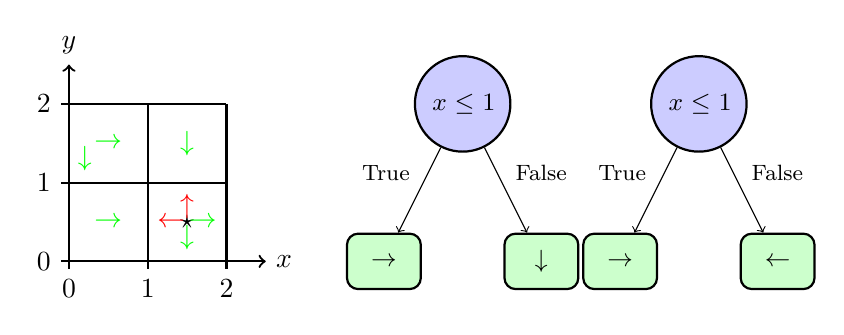
\begin{tikzpicture}[
        decision/.style={circle, draw, thick, fill=blue!20, text width=2.5em, text centered, minimum height=2.5em, font=\small},
        leaf/.style={rectangle, draw, thick, fill=green!20, text width=2em, text centered, rounded corners, minimum height=2em, font=\small},
        edge_label/.style={font=\footnotesize, midway}
    ]
        % Tree 4: if x <= 0.5 move right else move left
        \node[decision] (tree4_root) at (8,2) {$x \leq 1$};
        \node[leaf] (tree4_right) at (7,0) {$\rightarrow$};
        \node[leaf] (tree4_left) at (9,0) {$\leftarrow$};
        \draw[->] (tree4_root) -- (tree4_right) node[edge_label, above left] {True};
        \draw[->] (tree4_root) -- (tree4_left) node[edge_label, above right] {False};
        \tikzstyle{grid}=[draw, thick, fill=gray!10]


        % Tree 4: if x <= 0.5 move right else move left
        \node[decision] (tree5_root) at (5,2) {$x \leq 1$};
        \node[leaf] (tree5_right) at (4,0) {$\rightarrow$};
        \node[leaf] (tree5_left) at (6,0) {$\downarrow$};
        \draw[->] (tree5_root) -- (tree5_right) node[edge_label, above left] {True};
        \draw[->] (tree5_root) -- (tree5_left) node[edge_label, above right] {False};
        \tikzstyle{grid}=[draw, thick, fill=gray!10]
        
        % Draw grid
        \draw[grid] (0,0) grid (2,2);
        
        % Add axes
        \draw[thick, ->] (0,0) -- (2.5,0) node[right] {$x$};
        \draw[thick, ->] (0,0) -- (0,2.5) node[above] {$y$};
        
        % Add tick marks and labels
        \foreach \x in {0,1,2} {
            \draw[thick] (\x,0) -- (\x,-0.1) node[below] {$\x$};
        }
        \foreach \y in {0,1,2} {
            \draw[thick] (0,\y) -- (-0.1,\y) node[left] {$\y$};
        }
        
        % Add state labels clockwise from bottom left
        \node at (0.5,0.5) {{\color{green} $\rightarrow$}};
        \node at (1.5,0.5) {$\star$};
        \node at (1.5,0.7) {{\color{red} $\uparrow$}};
        \node at (1.5,0.3) {{\color{green} $\downarrow$}};
        \node at (1.7,0.5) {{\color{green} $\rightarrow$}};
        \node at (1.3,0.5) {{\color{red} $\leftarrow$}};
        \node at (1.5,1.5) {{\color{green} $\downarrow$}};
        \node at (0.2,1.3) {{\color{green} $\downarrow$}};
        \node at (0.5,1.5) {{\color{green} $\rightarrow$}};

    \end{tikzpicture}
    \caption{Grid world MDP optimal actions. An optimal policy that takes any of the red actions in the bottom right state might not be imitated by the best depth-1 tree in terms of performance interpretability trade-offs.
    Center, an optimal depth-1 decision tree policy. On the right, a sub-optimal depth-1 decision tree policy.}
    \end{figure}

\begin{figure}
    \centering
    \includegraphics[width=0.6\textwidth]{images/images_part1/policy_values_comparison.pdf}
    \caption{MDP objective values.}\label{fig:objectives}
\end{figure}

\begin{figure}
    \centering
    \includegraphics[width=1\textwidth]{images/images_part1/base_mdp.pdf}
    \caption{Left, sample complexity curve of Q-learning with default hyperparameters on the $2\times 2$ grid world MDP over 100 random seeds. Right, performances of indirect interpretable methods when imitating the greedy policy with a tree at different Q-learning stages. }
\end{figure}

\section{Iterative Bounding Markov Decision Processes}
In 2021, Topin et. al. introduced Iterative Bouding Markov Decision Processes (IBMDPs) with the promise of shifting the challenges of non-parametric decision tree policy learning in the problem formulation rather than in the design of specialized reinforcement learning algorithms.
Given a base MDP for which one wants to learn a decision tree policy, IBMDPs are an augmented version of this base MDP with more state features, more actions, additinal reward signal, and additional transition kernel.
Authors showed that certain IBMDP policies, that can be learned with RL, are equivalent to decision tree policies for the base MDP. 
\subsection{Formalism}
The key thing to know about IBMDPs is that they are, as their name suggests, MDPs. Hence they inherit all their properties such as existence of a deterministic optimal Markovian policy.
The states in an IBMDP are concatenations of base MDP states and some observations. Those observations are information about the base states that are refined--``iteratively bounded''-- at each step and represent a subspace of the base MDP state space.
Actions available in an IBMDP are the actions of the base MDP, that change the state of the latter, and \textit{information gathering} actions that change the observation part of the IBMDP state.
Now, taking base actions in an IBMDP is rewarded like in the base MDP, this ensures that the base objective, e.g. balancing the pole or treating cancer, is still encoded in the IBMDP reward. When taking such \textit{information gathering} actions; the reward is an arbitrary value supposed to trade-off between performance and interpretability.
 
Before showing how to get decision trees from IBMDP policies, we give a formal definition of the latter following Topin et. al. (cite).

\begin{definition}[Iterative Bounding Markov decision process]
Given a \textit{factored} (cite) MDP $\mathcal{M}$ (cite), that is, a tuple $\langle S, A, R, T, T_0 \rangle$ with $S\subsetneq \mathbb{R}^n$, an Iterative Bouding MDP $\mathcal{M}_ib$ is a tuple:
\begin{align*}
    \langle \overbrace{S, O}^{\text{State space}}, \underbrace{A, A_{info}}_{\text{Action space}}, \overbrace{R, \zeta}^{\text{Reward function}}, \underbrace{T_{info}, T, T_0}_{\text{Transition kernels}}\rangle
\end{align*}

\begin{itemize}
\item $S$ the base MDP state space should be of the form $S = [L_1, U_1]\times \dots \times [L_n, U_n]$ with $\infty < L_i \leq U_i < \infty \forall 1\leq i\leq n$.
\item $O$ are the observations in an IBMDP. They are partial information about the values of base MDP states: $O\subsetneq S^2 =  [L_1, U_1]\times \dots \times [L_n, U_n] \times [L_1, U_1]\times \dots \times [L_n, U_n]$. So the complete IBMDP state space is $(S, O) = S \times O$ the concatenations of states and observations.
\item $A$ are the actions of the base MDP.
\item $A_{info}$ are added \textit{information gathering} actions (IGAs) of the form $\langle i, v \rangle$ where $i$ is a state feature index $1 \leq i \leq n$ and $v$ is a real number. So the complete action space of an IBMDP is the set of base actions and \textit{information gathering} actions $A \cup A_{info}$.
\item $R: S\times A \rightarrow \mathbb{R}$ is the base MDP reward function that maps base states and actions to a real-valued reward signal.
\item $\zeta$ is a reward signal for taking an \textit{information gathering} action. So the IBMDP reward function is to get a reward from the base MDP if the action is a base MDP action or to get $\zeta$ if the action is a \textit{information gathering} action.
\item $T_{info}: S\times O \times( A_{info} \cup A )\rightarrow \Delta (S\times O)$ is the transition kernel of IBMDPs. 
Given the current observation $o_{t} = (L'_1, U'_1, \dots, L'_n, U'_n)\in O$ and the current state is $s_t=(s_1, s_2, \dots, s_n)$ if an AIG $\langle i, v \rangle$ is taken, only the bounds in the observation change:
\begin{align*}
    o_{t+1} &= \begin{cases}
        (L'_1, U'_1, \dots , L'_i, \min\{v, U'_i\}, \dots , L'_n, U'_n) \text{ if } s_i \leq v\\
        (L'_1, U'_1, \dots , \max\{v, L'_i\}, U'_i, \dots , L'_n, U'_n) \text{ if } s_i > v
    \end{cases}
\end{align*}
If a base action $a\in A$ is taken, $o_{t+1}$ is reset to the default state bounds $(L_1, U_1,\dots, L_n, U_n)$ and the base state changes according to the base MDP transitition kernel: $s_{t+1}\sim T(s, a)$.
At initialization, the base part of the IBMDP states is drawn from $T_0$ and the observation is set always set to $(L_1, U_1,\dots, L_n, U_n)$.
The overall IBMDP transitions are given by either $T_{info}$, which i fully deterministic, if an IGA is played, and by the base MDP's transition kernel otherwise.
\end{itemize}
\end{definition}
Now remains to extract a decision tree policy for $\mathcal{M}$ from a policy for IBMDP $\mathcal{M}_{IB}$. 

\subsection{From Policies to Trees}
\begin{algorithm}[t]
    \KwData{IBMDP policy $\pi$ and observation $o=(L'_1, U'_1, \dots, L'_n, U'_n)$}
    \KwResult{Decision tree policy extracted from $\pi$}
    
    \SetKwProg{Fn}{Function}{:}{}
    \SetKwFunction{SubtreeFromPolicy}{Subtree\_From\_Policy}
    
    \Fn{\SubtreeFromPolicy{$o, \pi$}}{
        $a \leftarrow \pi(o)$ \\
        \If{$a \in A_{info}$}{
            \Return Leaf\_Node(action: $a$) \Comment{// Leaf if base action}
        }
        \Else{
            $\langle i, v\rangle \leftarrow a$ \Comment{// Splitting action is feature and value} \\
            $o_L \leftarrow o; \quad o_R \leftarrow o$ \\
                         $o_L \leftarrow (L'_1, U'_1, \dots, L'_i, v, \dots, L'_n, U'_n); \quad o_R \leftarrow (L'_1, U'_1, \dots, v, U'_i, \dots, L'_n, U'_n)$ \\
            $child_L \leftarrow$ Subtree\_From\_Policy$(o_L, \pi)$ \\
            $child_R \leftarrow$ Subtree\_From\_Policy$(o_R, \pi)$ \\
            \Return Internal\_Node(feature: $i$, value: $v$, children: $(child_L, child_R)$)
        }
    }
    
    \caption{Extract a Decision Tree Policy from an IBMDP policy $\pi$, beginning traversal from $obs$.}\label{alg_extract_tree}
\end{algorithm}

One can notice that \textit{information gathering} actions resemble the Boolean functions that make up internal decision tree nodes (cite). 
Indeed, an agent evolving in an IBMDP essentially builds a tree by taking sequences of IGAs (internal nodes) and then a base action (leaf node) and repeats this process over time.
However not all IBMDP policies are decision tree policies. In particular, only deterministic policies depending solely on the observation part of the IBMDP states $\pi: O \rightarrow A\cup A_{info}$ are decision tree policies $\pi_{\mathcal{T}}: S \rightarrow A$ for the base MDP (cite).
Algorithm (cite) from (cite) extracts a decision tree policy for the base MDP from a determenistic partailly observable IBMDP policy.

\subsection{Didactic example}
We now present a didactic example of how some policies in IBMDPs correspond to a decision tree policy. 
Suppose a factored MDP representing a grid world with 4 cells (cite). The state space is $S = \{(0.5, 0.5), (0.5, 1.5), (1.5, 1.5), (1.5, 0.5)\}\subsetneq [0, 2] \times [0, 2]$.
The actions space are the cardinal directions $A = \{\rightarrow, \leftarrow, \downarrow, \uparrow\}$ that shift the states by one as long as the coordinates remain in the grid.
The reward for taking any action is 0 except when in the bottom right state $s_g = (1.5, 0.5)$ which is an absorbing state: once in this state, you stay there forever. 

In Figure (cite), we present how trajectories in IBMDP correspond to a decision tree policy.
We build an IBMDP with two information gathering actions and nine observations.
\begin{itemize}
    \item $\langle x, 1\rangle$ that tests if $x\leq 1$
    \item $\langle y, 1\rangle$ that tests if $y\leq 1$
\end{itemize}
The observations are induced by these to IGAs. The initial observation is $o_0=(0, 2, 0, 2)$.
The set of observations is finite and can be inferred from the possible bounds over the base states induced by the IGAs.
For example when starting in state $s_1 = (0.5, 1.5)$, and taking first $\langle x, 1\rangle$ then $\langle y, 1\rangle$ the corresponding observations are first $o_1 = (0, 1, 0, 2)$ and then $o_2 = (0, 1, 1, 2)$.
The full observation set is $O = \{(0, 2, 0, 2), (0, 1, 0, 2), (0, 2, 0, 1), (0, 1, 0, 1), (1, 2, 0, 2), (1, 2, 0, 1), (1, 2, 1, 2), (0, 1, 1, 2), (0, 2, 1, 2)\}$.
The transitions and rewards are given by definition (cite).
\begin{figure}[h]
\centering
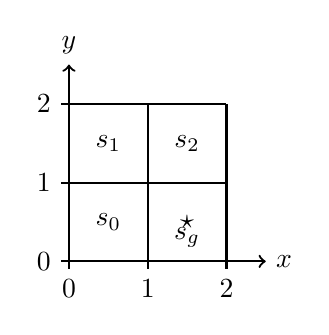
\begin{tikzpicture}
    \tikzstyle{grid}=[draw, thick, fill=gray!10]
    
    % Draw grid
    \draw[grid] (0,0) grid (2,2);
    
    % Add axes
    \draw[thick, ->] (0,0) -- (2.5,0) node[right] {$x$};
    \draw[thick, ->] (0,0) -- (0,2.5) node[above] {$y$};
    
    % Add tick marks and labels
    \foreach \x in {0,1,2} {
        \draw[thick] (\x,0) -- (\x,-0.1) node[below] {$\x$};
    }
    \foreach \y in {0,1,2} {
        \draw[thick] (0,\y) -- (-0.1,\y) node[left] {$\y$};
    }
    
    % Add state labels clockwise from bottom left
    \node at (0.5,0.5) {$s_0$};
    \node at (1.5,0.5) {$\star$};
    \node at (1.5,0.3) {$s_g$};
    \node at (1.5,1.5) {$s_2$};
    \node at (0.5,1.5) {$s_1$};
\end{tikzpicture}
\caption{A grid world MDP state space: it is a $2\times2$ grid.}
\end{figure}

\begin{figure}[h]
\centering
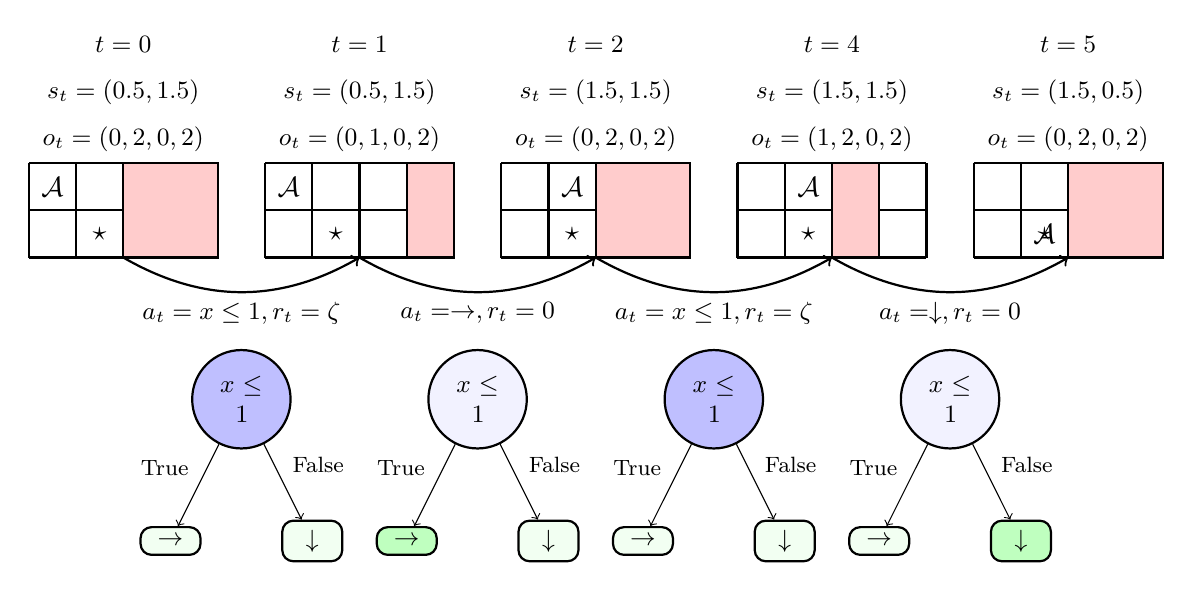
\begin{tikzpicture}[scale=0.6]
    % Define styles
    \tikzstyle{grid}=[draw, thick, fill=gray!10]
    \tikzstyle{rectangle}=[draw, thick, fill=red!20]
    
    % Row 1: IBMDP States (s, o)
    % t=0: Initial state
    \node at (2,8.5) {\small $t=0$};
    \node at (2,7.5) {\small $s_t=(0.5, 1.5)$};
    \node at (2,6.5) {\small $o_t=(0, 2, 0, 2)$};

    \draw[grid] (0,4) grid (2,6);
    \node at (0.5, 5.5) {$\mathcal{A}$};
    \node at (1.5, 4.5) {$\star$};

    \draw[rectangle] (2,4) rectangle (4,6);  
    
    % Curved arrow from t=0 to t=1
    \draw[thick, ->] (2,4) to[bend right=30] node[midway, below] {\small $a_t = x \leq 1, r_t = \zeta$} (7,4);

    % % t=1: After AIG x≤0.5
    \node at (7,8.5) {\small $t=1$};
    \node at (7,7.5) {\small $s_t=(0.5, 1.5)$};
    \node at (7,6.5) {\small $o_t=(0, 1, 0, 2)$};

    \draw[grid] (5,4) grid (7,6);
    \node at (5.5, 5.5) {$\mathcal{A}$};
    \node at (6.5, 4.5) {$\star$};

    \draw[grid] (7,4) grid (9,6);
    \draw[rectangle] (8,4) rectangle (9,6);

    % Curved arrow from t=1 to t=2
    \draw[thick, ->] (7,4) to[bend right=30] node[midway, below] {\small $a_t = \rightarrow, r_t = 0$}(12,4);

    \node[circle, draw, thick, fill=blue!25, text width=2em, text centered, minimum height=1.5em, font=\small] (tree4_root) at (4.5,1) {$x \leq 1$};
    \node[rectangle, draw, thick, fill=green!5, text width=1.5em, text centered, rounded corners, minimum height=1em, font=\small] (tree4_right) at (3,-2) {$\rightarrow$};
    \node[rectangle, draw, thick, fill=green!5, text width=1.5em, text centered, rounded corners, minimum height=1em, font=\small] (tree4_left) at (6,-2) {$\downarrow$};
    \draw[->] (tree4_root) -- (tree4_right) node[font=\footnotesize, midway, above left] {True};
    \draw[->] (tree4_root) -- (tree4_left) node[font=\footnotesize, midway, above right] {False};

    \node at (12,8.5) {\small $t=2$};
    \node at (12,7.5) {\small $s_t=(1.5, 1.5)$};
    \node at (12,6.5) {\small $o_t=(0, 2, 0, 2)$};
    
    \draw[grid] (10,4) grid (12,6);
    \node at (11.5, 5.5) {$\mathcal{A}$};
    \node at (11.5, 4.5) {$\star$};
    \draw[rectangle] (12,4) rectangle (14,6);
    
    % Curved arrow from t=2 to t=4
    \draw[thick, ->] (12,4) to[bend right=30] node[midway, below] {\small $a_t = x \leq 1, r_t = \zeta$} (17,4);

    \node[circle, draw, thick, fill=blue!5, text width=2em, text centered, minimum height=1.5em, font=\small] (tree4_root) at (9.5,1) {$x \leq 1$};
    \node[rectangle, draw, thick, fill=green!25, text width=1.5em, text centered, rounded corners, minimum height=1em, font=\small] (tree4_right) at (8,-2) {$\rightarrow$};
    \node[rectangle, draw, thick, fill=green!5, text width=1.5em, text centered, rounded corners, minimum height=1em, font=\small] (tree4_left) at (11,-2) {$\downarrow$};
    \draw[->] (tree4_root) -- (tree4_right) node[font=\footnotesize, midway, above left] {True};
    \draw[->] (tree4_root) -- (tree4_left) node[font=\footnotesize, midway, above right] {False};

    
    \node at (17,8.5) {\small $t=4$};
    \node at (17,7.5) {\small $s_t=(1.5, 1.5)$};
    \node at (17,6.5) {\small $o_t=(1, 2, 0, 2)$};

    \draw[grid] (15,4) grid (17,6);
    \node at (16.5, 5.5) {$\mathcal{A}$};
    \node at (16.5, 4.5) {$\star$};
    \draw[grid] (17,4) grid (19,6);
    \draw[rectangle] (17,4) rectangle (18,6);
    
    \draw[thick, ->] (17,4) to[bend right=30] node[midway, below] {\small $a_t = \downarrow, r_t = 0$} (22,4);
    
    \node[circle, draw, thick, fill=blue!25, text width=2em, text centered, minimum height=1.5em, font=\small] (tree4_root) at (14.5,1) {$x \leq 1$};
    \node[rectangle, draw, thick, fill=green!5, text width=1.5em, text centered, rounded corners, minimum height=1em, font=\small] (tree4_right) at (13,-2) {$\rightarrow$};
    \node[rectangle, draw, thick, fill=green!5, text width=1.5em, text centered, rounded corners, minimum height=1em, font=\small] (tree4_left) at (16,-2) {$\downarrow$};
    \draw[->] (tree4_root) -- (tree4_right) node[font=\footnotesize, midway, above left] {True};
    \draw[->] (tree4_root) -- (tree4_left) node[font=\footnotesize, midway, above right] {False};


    \node at (22,8.5) {\small $t=5$};
    \node at (22,7.5) {\small $s_t=(1.5, 0.5)$};
    \node at (22,6.5) {\small $o_t=(0, 2, 0, 2)$};
 
    \draw[grid] (20,4) grid (22,6);
    \node at (21.5, 4.5) {$\mathcal{A}$};
    \node at (21.5, 4.5) {$\star$};
    \draw[rectangle] (22,4) rectangle (24,6);

    \node[circle, draw, thick, fill=blue!5, text width=2em, text centered, minimum height=1.5em, font=\small] (tree4_root) at (19.5,1) {$x \leq 1$};
    \node[rectangle, draw, thick, fill=green!5, text width=1.5em, text centered, rounded corners, minimum height=1em, font=\small] (tree4_right) at (18,-2) {$\rightarrow$};
    \node[rectangle, draw, thick, fill=green!25, text width=1.5em, text centered, rounded corners, minimum height=1em, font=\small] (tree4_left) at (21,-2) {$\downarrow$};
    \draw[->] (tree4_root) -- (tree4_right) node[font=\footnotesize, midway, above left] {True};
    \draw[->] (tree4_root) -- (tree4_left) node[font=\footnotesize, midway, above right] {False};

    

    
\end{tikzpicture}
\caption{An IBMDP trajectory when the base MDP is 2$\times$2 grid world, and equivalent decision tree policy traversal. At $t=0$, the agent is in $s_1 = (0.5, 1.5)$. The initial observation is always the base MDP state bounds, here $(0, 2, 0, 2)$ because the base states are in $[0, 2] \times [0, 2]$. The agent takes an information gathering action in $A_{info}$ that tests the feature $x$ of the states against the value $1$. For that, the agent receives reward $\zeta$. This transition corresponds to going through an internal node in a decision tree policy as illustrated in the figure. At $t=1$, after gathering the information that the $x$-value of the current base state is below 1, the observation is updated with the refined state bounds $o_t=(0, 1, 0, 2)$ and the base state remains unchanged. The agent then takes a base action that is to move right. This gives a reward 0, reinitialized the observation to the original bounds, and changes the base state to $s_t=(1.5, 1.5)$. And the trajectory continues like this until the agent reaches the absorbing state $s_g=(1.5, 0.5)$.}
\label{fig:poibmdp_trajectory}
\end{figure}



\subsection{Partially Observable IBMDPs}

Now we know that to find a decision tree policy for a given MPD $\mathcal{M}$ satisfying the definition (cite); one has to find a partially observable--sometimes called \textit{memoryless} or \textit{reactive}--deterministic policy for an IBMDP $\mathcal{M}_{IB}$.
Such problems are classical instances of Partially Observable Markov Decision Processes (POMDPs) (cite). This connection with POMDP was not done by the authors of IBMDPs. 

\begin{definition}[Partially Observable Markov Decision Processes]
A Partially Observable Markov Decision Process (POMDP) is a tuple $\langle X, A, O, T, T_0, \Omega, R\rangle$ where:
\begin{itemize}
    \item $X$ is the state space (like in the base definition of MDPs).
    \item $A$ is a finite set of actions (like in the base definition of MDPs).
    \item $O$ is a set of observations.
    \item $T: X \times A \rightarrow \Delta X$ is the transition kernal, where $T(s, a, x') = P(x'|x, a)$ is the probability of transitioning to state $x'$ when taking action $a$ in state $x$
    \item $T_0$: is the intial distribution over states. 
    \item $\Omega: X \rightarrow \Delta O$ is the observation kernel, where $\Omega(x', a, o) = P(o|x', a)$ is the probability of observing $o$ in state $x$
    \item $R: X \times A \rightarrow \mathbb{R}$ is the reward function, where $R(x, a)$ is the immediate reward for taking action $a$ in state $x$
\end{itemize}
Note that $\langle X, A, R, T, T_0 \rangle$ defines an MDP (cite).
\end{definition}

We can simply extend the definition of Iterative Bounding MDPs (cite) with an observation kernel to get Partially Observable IBMDPs:
\begin{definition}[Partially Observable Iterative Bounding Markov Decision Processes] a Partially Observable Iterative Bounding Markov Decision Process (POIBMDP) is a an IBMDP (cite) extended with an observation kernel 
    \begin{align*}
        \langle \overbrace{S, \underbrace{O}_{\text{Observations}}}^{\text{fully observable states X}}, \underbrace{A, A_{info}}_{A}, \overbrace{R, \zeta}^{R}, \underbrace{T_{info}, T, T_0}_{T, T_0}, \Omega \rangle
    \end{align*}
\end{definition}

The sole specifity of POIBMDPs compared to the general definition of POMDPs, is that $\Omega(o|(s, o'))$, the probability of observing $o$ in $(s,o')$, is $1_{o=o'}$.
This particular instance of POMDPs with observations being some indices of the fully-observable states has other names in the litterature: Mixed Observability MDPs (cite), Block MDPs (cite).
POIBMDPs can also be seen as non-stationary MDPs in which there is one different transition kernel per base MDP state: these are called Hidden-Mode MDPs (cite). 

Following (cite) we can write the definition of the value of a deterministic partially observable policy $\pi:O\rightarrow A$ in observation $o$.

\begin{definition}[Partial observable value function] In a POIBMDP, the expected cumulative discounted reward of a deterministic partially observable policy $\pi:O\rightarrow A\cup A_{info}$ starting from observation $o$ is $V^{\pi}(o)$:
    \begin{align*}
        V^{\pi}(o) &= \underset{(s,o')\in S\times O}{\sum}P^{\pi}((s, o')|o)V^{\pi}((s, o'))
    \end{align*}
with $P^{\pi}((s, o')|o)$ the asymptotic occupancy distribution (see cite for definition) of the fully observable state $(s,o')$ given the partial observation $o$ and $V^{\pi}((s, o'))$ the classical state-value function defined in (cite).
\end{definition}


The asymptotic occupancy distribution is the probability of a policy $\pi$ to be in $(s,o')$ while observing $o$ and having taken actions given by $\pi$.  

The problem that we solve is to find the deterministic partially observable policy that maximizes the excpeted value in the initial observation:
\begin{align}
    \pi^{\star} &= \underset{\pi}{\operatorname{argmax}}J(\pi) = \underset{\pi}{\operatorname{argmax}}V^{\pi}(o_0)
\end{align}
With $\pi:O\rightarrow A\cup A_{info}$. There is no expectation over possible initial observation in the above objective function as there is only one initial observation in a POIBMDP: $o_0=(L_1, U_1, \dots, L_n, U_n)$.

This particular problem of learning deterministic partially observable policies for POMDPs has been studied in the works of Littman, Singh and Jordan: (cite).
In (cite) atuhors give som intution behind why the above optimization problem is hard. For example, the optimal partially observable policy can be stochastic (cite precise section), hence policy gradient algoriothms (cite) are to avoid. 
Furthermore, the optimal deterministic patially observable policy might not maximize all the value of all observations simulataneously (cite precise section) which makes difficult the use the Bellman optimality equation (cite) to compute policies.
Despite those hardness results, empirical results of applying RL to POMDPs by naively setting the states to be observations has shown promising results (cite). 
More recently, the framework of Baisero et. al. (cite) called asymmetric RL has also shown promising empirical and theoretical results when leveraging fully-observable state information during training of a partially observable policy.
In the next chapter, we use reinforcement learning to train decision tree policies for MDPs by seeking deterministic partially observable policies for POIBMDPs (cite).  
\begin{figure}[h]
\centering
\begin{tikzpicture}
    \draw[fill=blue!40] (0, 0) rectangle (6, 4);
    \node at (3, 3.5) {POIBMDP $\mathcal{M}_{POIB}\langle\mathcal{M}_{IB}, \Omega\rangle$};
    \draw[fill=blue!30] (0, 0) rectangle (5.9, 3);
    \node at (3, 2.5) {IBMDP $\mathcal{M}_{IB} \langle \mathcal{M}, O, A_{info}, \zeta, T_{info}\rangle$};
    \draw[fill=blue!10] (0, 0) rectangle (5, 2);
    \node at (3, 1.5) {MDP $\mathcal{M} \langle S, A, R, T, T_0 \rangle$};
    
    \draw[fill=red!10] (10, 0) rectangle (14, 3);
    \node at (12, 2) {\textbf{Objective}};
    \node at (12, 1) {$\pi^{\star} = \underset{\pi}{\operatorname{argmax}} V^{\pi}(o_0)$};
    
    \draw[fill=red!10] (1, -5) rectangle (5, -2);
    \node at (3, -3) {\textbf{Decision Tree Policy}};
    \node at (3, -4) {$\pi_{\mathcal{T}}: S \rightarrow A$};
    
    \draw[fill=red!10] (9.5, -5) rectangle (14.5, -2);
    \node at (12, -3) {\textbf{Deterministic PO Policy}};
    \node at (12, -4) {$\pi: O \rightarrow A \cup A_{info}$};
    
    \draw[thick, ->] (6, 2) -- (10, 2) node[midway, above] {$\gamma$};
    \draw[thick, <-] (5, -3.5) -- (9.5, -3.5) node[midway, above] {Extract tree with Alg 6};
    \draw[thick, ->] (12, 0) -- (12, -2) node[midway, left] {Solve with e.g. RL};
    \draw[thick, <-] (3, 0.5) -- (3, -2) node[midway, left] {Can be interpreted};

    
    % % Final arrow from tree back to base MDP - adjusted position
    % \draw[thick, ->] (1.75, -2.5) -- (1.75, -0.5) node[midway, right] {Can deploy\\and interpret};
    
\end{tikzpicture}
\caption{A formal framework to learn decision tree policies for MDPs. This include learning a partially observable deterministic policy in a POIBMDP (cite).}
\label{fig:nested_decision_processes}
\end{figure}


\chapter{A Case Study of Direct Deep Reinforcement Learning of Decision Tree Policies}
In this chapter compare direct reinforcement learning of decision tree policies to imitation learning (cite) of decision tree policies.
We follow the methodology introduced in (cite) and summarized in Figure (cite) to learn decision tree policies for the CartPole control problem.
In particular, we attempt to reproduce the results from Table (cite) in which authors use imitation learning or deep reinforcement learning in IBMDPs to directly learn a detph-2 decision tree for the CartPole control.

We run the \textit{same} algorithms using the \textit{same} hyperparameters when possible and show our results differ from (cite) in that we find that direct interpretable reinforcement learning underperforms compared to the indirect approach (cite).

\section{Reproducing ``Iterative Bounding MDPs: Learning Interpretable Policies via Non-Interpretable Methods''}

\subsection{IBMDP formulation}
As described in (cite), given a base MDP $\mathcal{M}\langle S, A, R, T, T_0\rangle$, in order to define an IBMDP $\mathcal{M}_{IB}\langle S\times O, A\cup A_{\info}, (R, \zeta),( T, T_0, T_{info})\rangle$, the user needs to provide the set of information gathering actions $A_{info}$ and the reward $\zeta$ for taking those.

For CartPole and other MDPs with large state spaces, authors propose to parametrize the set of IGAs with $i \times p$ actions $\langle v_k, i \rangle$ with $v_k$ depending on the current observation $\boldsymbol{o}_t=(L'_1, U'_1, \dots, L'_i, U'_i, \dots, L'_n, U'_n)$: $v_k = \frac{k(U'_i - L'_i)}{p+1}$.
This parametric IGAs space keeps the discrete IBMDP action space at a reasonable size while providing a learning agent with very veried tests.

For example, if we define an IBMDP with $p=3$ for the grid world IBMDP from Example (cite), at every time six actions are available. 
At $t=0$, recall that $\boldsymbol{o}_0=(0, 2, 0, 2)$, so if an agent takes, e.g., IGA $\langle v_2, 2 \rangle$, the effective IGA is $\langle v_2=\frac{k(2-0)}{3+1}, i \rangle = \langle 1, 2 \rangle$ which in turn effectively corresponds to an internal decision tree node $y \leq 1$.
If the current state $y$-feature value is $0.5$, then the next observation at $t=1$ is $\boldsymbol{o}_1=(0, 2, 0, 1)$. At $t=2$ if $a_t=\langle v_2, 2 \rangle$ again, it would be effectively $\langle v_2=\frac{k(1-0)}{3+1}, i \rangle = \langle 0.5, 2 \rangle$. 
This would give the next observation at $t=2$ $\boldsymbol{o}_2=(0, 2, 0, 0.5)$ and so on \dots. 

Furthermore, author propose to regularize the learned decision tree policy with a maximum depth parameter $D$.
Unfortunately, authors did not describe how they implemented the depth control in their work, hence we have to try different approaches to reproduce their results.

To control the tree depth during learning we can either give negative reward for taking $D$ IGAs since the last base action, or we could terminate the trajectory. 
The penalization approaches can break the MDP formalism because the reward function now depends on time while it should only depend on states and actions (cite). 
Similarly, the termination approach requires a transition function that depends on time breaking the Makrov property.

We actually find that when $p+1$, the IBMDP information gathering space parameter, is a prime number, then as a direct consequence of the \textit{Chinese Reminder Theorem} (cite)(proof), the current tree depth is directly encoded in the current observation $o_t$. 
Hence, when $p+1$ is prime, we can control the depth through trnasitions or rewards without tracking the time.

We will try various $\zeta$, various $p$ and various depth control approaches in our experiments but first we describe the reinforcement learning agents.


\subsection{Modified Deep Reinforcement Learning algorithms}
Authors of (cite) use two deep reinforcement learning baselines to which they apply some modifications in order to learn partially observable policies as required by proposition (cite).

The first algorithm is a modified proximal policy optimization algorithm (PPO)(cite)(algo).
To satisfy proposition (cite) authors modify the default PPO and train a neural network policy $O\rightarrow A\cup A_{info}$ while the neural network value function is $S\times O\rightarrow A\cup A_{info}$ like in the traditional PPO.

The second deep reinforcement learning algorithm used is the deep Q-networks algorithm (DQN) (cite)(algo).
A similar modification is done to DQN to work with partially observable policy. The trained $Q$-function is approximated with a neural network $O\rightarrow \rightarrow \mathbb{R}^{|A\cup A_{info}|}$ rather than $S\times O\rightarrow \mathbb{R}^{|A\cup A_{info}|}$.
In this modified DQN, the temporal difference error target for the $Q$-function $O\rightarrow A\cup A_{info}$ is approximated by a neural network $S\times O\rightarrow A\cup A_{info}$ that is in turn trained by bootstrapping the temporal difference error with itself.

Those two variants of DQN and PPO have first been introduced in (PINTO) for robotics task and later studied theoretically to solve POMDPs (cite) in Baisero's work and we defer their connexions to direct interpretable reinforcement learning to the next Chapter.

Next, we present the precise experimental setup we use to reproduce the work of (cite) in order to study direct deep reinforcement learning of decision tree policies for the CartPole MDP.

\section{Experimental setup}
\subsection{(IB)MDP} 

We use the exact same MDP and associated IBMDP for our experiments as authors of (cite) except mentioned otherwise.

\paragraph{MDP} The problem at hand is the CartPole MDP. At each time step a learning agent observes the cart position velocity and the pole angle and angular velocity, and can take action to push the cart left or right. While the cart is roughly balanced, i.e., while the cart angle remains in some fixed range, the agent gets a positive reward.
If the cart is out of balance; the agent goes to an absorbing terminal state and gets 0 reward forever.
In practice, authors use the gymnasium \texttt{CartPole-v0} implementation (cite) of the CartPole MDP in which trajectories are truncated after 200 timesteps making the maximum cumulative reward over a trajectory to be 200.
Since the IBMDP definition requires the MDP state space to be a factor of bounded segments, authors bound the the state space of the CartPole MDP to be in $[-2, 2] \times [-2, 2] \times [-0.14, 0.14] \times [-1.4, 1.4]$.

\paragraph{IBMDP} Authors define the associated IBMDP with $\zeta=-0.01$ and parametric information gathering action space defined by $p=3$.
In addition we also try $\zeta=0.01$ and $p=2$.
The discount factor used by the authors is $\gamma=1$.

We potentially differ from the original paper setting in the way we handle maximum depth limiation. 
Indeed authors restrain the learning of policies to be equivalent to depth-2 trees but don't detail how they do so.
We hence try two different approaches as mentioned in the previous secion: terminating trajectories if the agent takes too much information gathering in a row or simply giving a reward of $-1$ to the agent everytime it takes an information gathering action past the depth limit.
We will also try IBMDPs where we do not limit the maximum depth for completeness.

\subsection{Baselines}
\paragraph{Modified DQN} as mentioned above, authors use a modified version (cite) of the DQN algorithm (cite).
We use the exact same hyperparameters for Modified DQN as the authors when possible. 
We use the same layers width (128) and number of hidden layers (2), the same exploration strategy ($\epsilon$-greedy with linarly decreasing value $\epsilon$ between 0.5 and 0.05 during the first 10\% of the training),
the same replay buffer size ($10^6$) and the same number of transitions to be collected randomly before doing value updates ($10^5$).
We also try to use more exploartion during training (change the initial $\epsilon$ value to 0.9).
We use the same optimizer (RMSprop (cite) with hyperparmeter 0.95 and learning rate $2.5 \times 10^{-4}$) to update the $Q$-networks.

Authors did not share what DQN implementation they used so we use the stable-baselines3 one (cite).
Authors did not share what activations they used so we try both $\operatorname{tanh}()$ and $\operatorname{relu}()$. 

\paragraph{Modified PPO} for the modified PPO algorithm, we can exactly match the authors hyperparameters since they use the open source stable-baselines3 implementation of PPO.

Similarly to authors of (cite) we train Modified DQN on 1 million timesteps and Modified PPO on 4 million timesteps.

\paragraph{DQN and PPO} We also benchmark the non-modified standard DQN and PPO when learning fully observable IBMDP policies $\pi:S\times O\rightarrow A\cup A_{info}$ and when learning standard $\pi:S\rightarrow A$ policies directly in the CartPole MDP.

We summarize hyperpameters for the IBMDP and for the learning algorithms in Tables (cite) and (cite).

\begin{table}[h]
    \centering
    \caption{IBMDP hyperparameters. We try 12 different IBMDPs. In \textcolor{green}{green} we highlight the hyperparameters from the original paper and in \textcolor{red}{red} we highlight the hyperparameter names for which author do not give information.}
    \begin{tabular}{ll}
    \toprule
    \textbf{Hyperparameter} & \textbf{Values}\\
    \midrule
    Discount factor $\gamma$ & \textcolor{green}{1} \\
    Information gathering actions parameter $p$ & 2, \textcolor{green}{3} \\
    Information gathering actions rewards $\zeta$ & \textcolor{green}{-0.01}, 0.01 \\
    \textcolor{red}{Depth control} & Done signal, negative reward, none \\ 
    \bottomrule
    \end{tabular}
    \end{table}

\begin{table}[h]
    \centering
    \caption{(Modified) DQN trained on $10^6$ timesteps. This gives four different instantiation of (modified) DQN. Hyperparameters not mentioned are stable-baselines3 default. In \textcolor{green}{green} we highlight the hyperparameters from the original paper and in \textcolor{red}{red} we highlight the hyperparameter names for which author do not give information.}
    \begin{tabular}{ll}
    \toprule
    \textbf{Hyperparameter} & \textbf{Values}\\
    \midrule
    Buffer size & \textcolor{green}{$10^6$} \\
    Random transitions before learning & \textcolor{green}{$10^5$} \\
    Epsilon stard & 0.9, \textcolor{green}{0.5} \\
    Epsilon end & \textcolor{green}{0.05} \\
    Exploration fraction & \textcolor{green}{0.1} \\
    Optimizer & \textcolor{green}{RMSprop ($\alpha = 0.95$)}\\
    Learning rate & \textcolor{green}{$2.5\times10^{-4}$}\\
    Networks architectures & \textcolor{green}{[128, 128]}\\
    \textcolor{red}{Networks activation} & $\operatorname{tanh()}$, $\operatorname{relu()}$\\
    \bottomrule
    \end{tabular}
    \end{table}

\begin{table}[h]
    \centering
    \caption{(Modified) PPO trained on $4\times10^6$ timesteps. This gives two different instantiation of (modified) PPO. Hyperparameters not mentioned are stable-baselines3 default. In \textcolor{green}{green} we highlight the hyperparameters from the original paper and in \textcolor{red}{red} we highlight the hyperparameter names for which author do not give information.}
    \begin{tabular}{ll}
    \toprule
    \textbf{Hyperparameter} & \textbf{Values}\\
    \midrule
    Steps between each policy gradient steps & \textcolor{green}{512} \\
    Number of minibatch for policy gradient updates & \textcolor{green}{4} \\
    Networks architectures & \textcolor{green}{[64, 64]}\\
    \textcolor{red}{Networks activations} & $\operatorname{tanh()}$, $\operatorname{relu()}$\\
    \bottomrule
    \end{tabular}
    \end{table}


\paragraph{Indirect methods} We also compare Modified RL algorithm to imitation learning.
To do so, we use Viper or Dagger (cite) to imitate greedy neural network policies obtained with standard DQN learning directly on CartPole.
And we use Dagger to imitate neural network policies obtained with the standard PPO learning directly on CartPole. 

For each indirect method, we imitate the neural network experts by fitting decision trees on 10000 expert transitions using the greedy tree classifier from scikit-learn with default hyperparameters and maximum depth of 2.
    

\subsection{Metrics}
The key metric of this section is performance when controlling the CartPole, i.e, the average undiscounted cumulative reward of a policy on 100 trajectories.

For Modified RL algorithms that learn a partially observable policy (or $Q$-function) in an IBMPD, we periodically extract the policy (or $Q$-function) and use Alg 6 (cite) to extract a decision tree for the CartPole MDP. 
We then evaluate the tree on 100 independent trajectories in the MDP and report the mean undiscounted cumulative reward.

For standard RL applied to IBMDPs, since we can't deploy learned policies directly to the base MDP as the state dimensions mismatch, we periodically evaluate those fully observable IBMDP policies periodically in a copy of the training IBMDP in which we fix $\zeta=0$ ensuring that the cumulative copied IBMDP reward only corresponds to rewards from the base CartPole MDP.
Similarly, we do 100 trajectories of the extracted policies in the copied IBMDP and report the average cumulative reward.

For RL applied directly to the base MDP we can just periodically extract the learned policies and evaluate them on 100 trajectories CartPole control trajectories.

Since imitation learning baselines train offline, i.e, on a fixed dataset, their performances cannot be reported on the same axis as RL baselines.
For that reason, during the training of a standard RL baseline, we periodically extract the trained neural policy/$Q$-function that we consider as the expert to imitate.
Those experts are then imitated with Viper or Dagger using 10 000 newly generated transitions and the fitted decision trees are then evaluated on 100 CartPole trajectories.

Every single combination of IBMDP and Modified RL hyperparameters is run 20 times.
For standard RL on either an IBMDP or an MDP with use the paper's original hyperparameters when they were spicified, with depth control using negative rewards, $\operatorname{tanh()}$ activations, and we repeat this training 20 times. 

Next, we present our results and discuss the reproducibility and limitations of the original approach presented in (cite).

\section{Results}

\subsection{How well do Modified Deep RL baselines learn in IBMDPs?}

\begin{figure}
    \centering
    \includegraphics[width=0.8\textwidth]{images/images_part1/dqn.pdf}
    \caption{Variations of Modified DQN, DQN, on CartPole IBMDP variations. We give different line-styles for the learning curves for DQN applied directly on CartPole and DQN applied on the IBMDP.
    Since there are multiple possible candidates for the original paper hyperparametrs, we choose to color the (Modified DQN variant, IBMDP variant) pair that resulted in the best decision tree policy on CartPole among the instances that could match the original paper.
    Shaded areas represent the confidence interval at 95\% at each measure on the y-axis.}
\end{figure}

\begin{figure}
    \centering
    \includegraphics[width=0.8\textwidth]{images/images_part1/ppo.pdf}
    \caption{Variations of Modified PPO, PPO, on CartPole IBMDP variations. We give different line-styles to the learning curves for PPO applied directly on CartPole and PPO applied on the IBMDP.
    Since there are multiple possible candidates for the original paper hyperparametrs, we choose to color the (Modified PPO variant, IBMDP variant) pair that resulted in the best decision tree policy on CartPole among the instances that could match the original paper.
    Shaded areas represent the confidence interval at 95\% measure on the y-axis.}
\end{figure}
On Figure (cite), we observe that Modified DQN can learn in IBMDPs--the curves have an increasing trend--but we also observe that Modified DQN finds poor decision tree policies for CartPole in average--the curves flatten at the end of the x-axis and have low y-values--.
In, particular, among all the learning curves that could possibly correspond to the original paper Modified DQN, the learning curve with highest final y-value is converging to decision tree policies for CartPole high poor performances.

On Figure (cite) we observe that Modified PPO finds decision tree policies with 150 cumulative rewards towrads the end of training. The performance difference with Modified DQN could be because we trained longer, like in the original paper.

However it could also be because DQN-like algorithm with those hyperpameters struggle in general CartPole MDP or IBMDPs.

Indeed, on Figures (cite) and (cite), we observe that baselines seeking fully observable policies (RL + IBMDP and RL + MDP), learn better CartPole policies in average for both DQN and PPO-like baselines. 
We do notice that for DQN-like baselines, learning seems difficult in general indepedently of the setting while on Figure (cite) it is clear that for PPO baselines seeking fully observable, learning is super efficient and agent find optimal policies with reward 200.

In Tables (cite) and (cite) we report the top-5 hyperparameters for Modified RL baselines when learning partially observable IBMDP policies in terms of extracted decision tree policies performances in CartPole control.
\begin{table}[h]
    \centering
    \caption{Top 5 Hyperparameter Configurations for Modified DQN + IBMDP, bold font represent the original paper hyperparameters.}
    \label{tab:top5_results}
    \begin{tabular}{ccccccS}
    \toprule
    Rank & $p$ & Depth control & Activation & Exploration & $\zeta$ & {Final Performance} \\
    \midrule
    1 & 3 & termination & $\operatorname{tanh}()$ & 0.9 & 0.01 & 53 \\
    2 & 2 & termination & $\operatorname{tanh}()$ & 0.5 & -0.01 & 24 \\
    \textbf{3} & \textbf{3} & \textbf{termination} & $\operatorname{tanh}()$ & \textbf{0.5} & \textbf{-0.01} & \textbf{24} \\
    4 & 2 & termination & $\operatorname{tanh}()$ & 0.5 & 0.01 & 23 \\
    5 & 2 & termination & $\operatorname{tanh}()$ & 0.9 & -0.01 & 22 \\
    \bottomrule
    \end{tabular}
    \end{table}

    \begin{table}[h]
        \centering
        \caption{Top 5 Hyperparameter Configurations for Modified PPO + IBMDP, bold font represent the original paper hyperparameters.}
        \label{tab:top5_ppo_results}
        \begin{tabular}{cccccS}
        \toprule
        Rank & $p$ & Depth Control & Activation & $\zeta$ & {Final Performance} \\
        \midrule
        1 & 3 & reward & $\operatorname{relu}()$ & 0.01 & 139 \\
        2 & 3 & done & $\operatorname{relu}()$ & 0.01 & 132 \\
        \textbf{3} & \textbf{3} & \textbf{reward} & $\operatorname{tanh}()$ & \textbf{-0.01} & \textbf{119} \\
        4 & 3 & reward & $\operatorname{relu}()$ & -0.01 & 117 \\
        5 & 3 & reward & $\operatorname{tanh}()$ & 0.01 & 116 \\
        \bottomrule
        \end{tabular}
        \end{table}


\subsection{How does direct interpretable reinforcement learning perform compared to the indirect approach?}

\begin{figure}
    \centering
    \includegraphics[width=1\textwidth]{images/images_part1/ppo_tree_study.pdf}
    \caption{(left) Mean performance of the best Modified PPO on the best IBMDP with shaded areas representing the min and max performance over the 20 seeds during training. (right) Histogram of the final decision tree policies performances.}
\end{figure}


\begin{figure}[htbp]
    \centering
    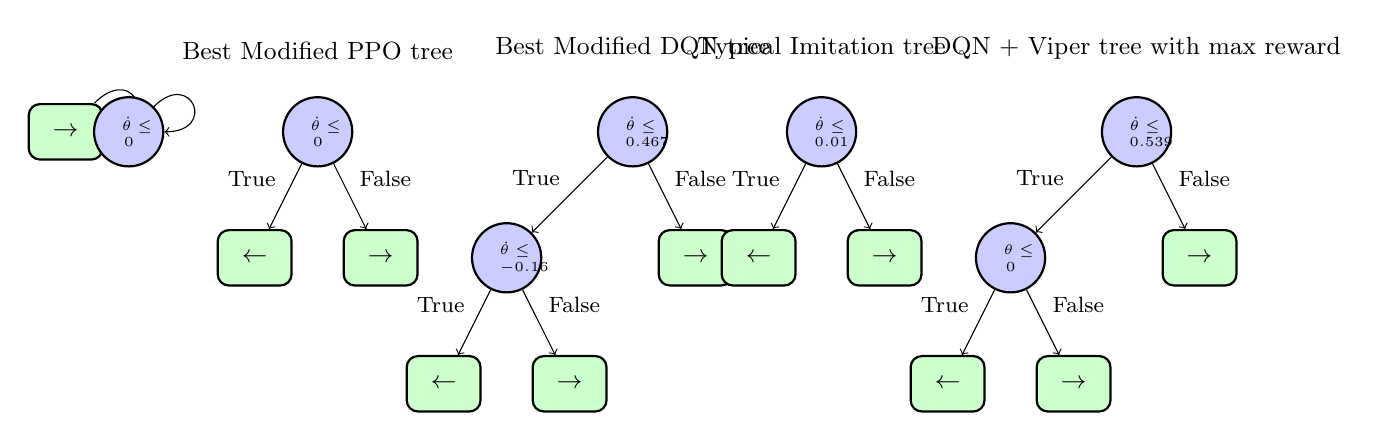
\begin{tikzpicture}[
        scale=0.8,
        decision/.style={circle, draw, thick, fill=blue!20, text width=0.5em, text centered, minimum height=2.5em, font=\tiny},
        leaf/.style={rectangle, draw, thick, fill=green!20, text width=2em, text centered, rounded corners, minimum height=2em, font=\small},
        edge_label/.style={font=\footnotesize, midway}
    ]

        \node[leaf] (tree7_root) at (-4,0) {$\rightarrow$};
        \draw[->] (tree7_root) to[out=45,in=0,looseness=5] (tree7_root);

        \node[decision] (tree7_root) at (-3,0) {$\dot{\theta} \leq 0$};
        \draw[->] (tree7_root) to[out=45,in=0,looseness=5] (tree7_root);
        
        % Tree 4: if x <= 0.5 move right else move left
        \node[decision] (tree4_root) at (0,0) { $\dot{\theta}\leq 0$};
        \node[leaf] (tree4_right) at (-1,-2) {$\leftarrow$};
        \node[leaf] (tree4_left) at (1,-2) {$\rightarrow$};
        \draw[->] (tree4_root) -- (tree4_right) node[edge_label, above left] {True};
        \draw[->] (tree4_root) -- (tree4_left) node[edge_label, above right] {False};
        

        % Tree 7: if x <= 0.5 and y <= 0.5 move right else move down
        \node[decision] (tree7_root) at (5,0) {$\dot{\theta}\leq 0.467$};
        \node[decision] (tree7_y) at (3,-2) {$\dot{\theta}\leq -0.16$};
        \node[leaf] (tree7_right) at (2,-4) {$\leftarrow$};
        \node[leaf] (tree7_down) at (4,-4) {$\rightarrow$};
        \node[leaf] (tree7_down2) at (6,-2) {$\rightarrow$};
        \draw[->] (tree7_root) -- (tree7_y) node[edge_label, above left] {True};
        \draw[->] (tree7_root) -- (tree7_down2) node[edge_label, above right] {False};
        \draw[->] (tree7_y) -- (tree7_right) node[edge_label, above left] {True};
        \draw[->] (tree7_y) -- (tree7_down) node[edge_label, above right] {False};




        % Tree 4: if x <= 0.5 move right else move left
        \node[decision] (tree4_root) at (8,0) { $\dot{\theta}\leq 0.01$};
        \node[leaf] (tree4_right) at (7,-2) {$\leftarrow$};
        \node[leaf] (tree4_left) at (9,-2) {$\rightarrow$};
        \draw[->] (tree4_root) -- (tree4_right) node[edge_label, above left] {True};
        \draw[->] (tree4_root) -- (tree4_left) node[edge_label, above right] {False};


        % Tree 7: if x <= 0.5 and y <= 0.5 move right else move down
        \node[decision] (tree7_root) at (13,0) {$\dot{\theta}\leq 0.539$};
        \node[decision] (tree7_y) at (11,-2) {$\theta\leq 0$};
        \node[leaf] (tree7_right) at (10,-4) {$\leftarrow$};
        \node[leaf] (tree7_down) at (12,-4) {$\rightarrow$};
        \node[leaf] (tree7_down2) at (14,-2) {$\rightarrow$};
        \draw[->] (tree7_root) -- (tree7_y) node[edge_label, above left] {True};
        \draw[->] (tree7_root) -- (tree7_down2) node[edge_label, above right] {False};
        \draw[->] (tree7_y) -- (tree7_right) node[edge_label, above left] {True};
        \draw[->] (tree7_y) -- (tree7_down) node[edge_label, above right] {False};
        


        % Labels
        \node[above] at (0,1) {{\small Best Modified PPO tree}};
        \node[above] at (5,1) {{\small Best Modified DQN tree}};
        \node[above] at (8,1) {{\small Typical Imitation tree}};
        \node[above] at (13,1) {{\small DQN + Viper tree with max reward}};


    \end{tikzpicture}
    \caption{Trees obtained by DRL against trees obtained with imitation.}
    \label{fig:trees-drl}
\end{figure}


On Figure (cite), we isolate the best performing baselines that learn decision tree policies for CartPole using either Modified DQN or Modified PPO and compare them with imitation learning baselines that use the surrogate objective (cite) to find CartPole decision tree policies.
We find that despite having poor performances in \textit{average} (c.f. Figure (cite)), the deep reinforcement learning baselines find very good decision tree policies and also extremly poor ones as shown by the min-max shaded areas on the left of Figure (cite) and the estimated density of final trees performances on Figure (cite).
In fact, when compared with imitation learning baselines, that fit the policy of a PPO + MDP or fit the greedy policy w.r.t to the $Q$-network of a DQN + MDP, when running e.g., 20 seeds of direct reinforcement learning baselines, there are some seeds that can find good decision tree policies as fast as the indirect imitation learning baselines: if we look at the shaded area of Modified DQN on Figure (cite), we can observe that it is consitently overlapping with an inderect method curve.
However this is not desirable, a user want an agent that can consistantly find good decision tree policy.
As shown by the estimated densities (cite), indirect methods consistently find good decision tree policies (the higher modes of distributions are on the right of the plot). On the other hand, the final trees returned by direct RL methods seem equally distributed on both extremes of the scores.

On Figure (cite), we compare the best trees returned by Modified DQN and Modified PPO. We used Algorithm 6 to extract 20 trees from the 20 partially observable policies returned by deeop reinforcement learning over 20 seeds. We then plot the best tree for each baseline. Those trees get an everage reward of roughly 175.
Similarly, we plot a representative tree for imitation learning baseline as well as a tree that has max reward obtained with Viper. 
However unlike for direct methods, the tree returned are extremely similar across seed. In particular they often only vary in the scalar value used in the root node but in general have the same structure and test the angular velocity.
On the other hand the most frequent tree across seed returned by modified RL baselines is the ``infinite'' tree that corresponds to only taking an information gathering action.


\section{Discussion}
We have shown that compared to learning non-interpretable policies for both the base MDP and some associated IBMDP, learning partially observable policies in IBMDP is difficult (c.f. Figures and (cite)). 
As a consequence, only a handful of Modified RL runs are able to learn decision tree policies that are on par with imitated trees (c.f. Figure).

In the next chapter, we highlkight the conncexions between RL in IBMDPs and POMDPs to get insights on the hardness of direct reinforcement learning of decision trees.
\chapter{Limits of direct reinforcement learning of decision tree policies}\label{sec:pomdp}

From the previous chapter, we know that to directly learn decision tree policies that optimize the RL objective (\ref{def:mdp-obj}) for an MDP, one can learn a deterministic partially observable policy that optimizes the interpretable RL objective (cf. definition~\ref{def:irl}) in an IBMDP (cf. definition~\ref{def:ibmdp} and proposition~\ref{def:po-policy}).
Such problems are classical instances of partially observable Markov decision processes (POMDPs)~\cite{POMDP,chap2}.
This connexion with POMDPs brings novel insights to direct reinforcement learning of decision tree policies. 
In this chapter, all the decision processes presented have a finite number of vector-valued states and observations.
Hence we will use bold fonts for states and observations but can still use summations rather than integrals when required.

\section{Partially observable iterative Markov decision processes}\label{sec:poibmdp}
A POMDP is an MDP where the current state is hidden; only some information about the current state is observable.

\begin{definition}[Partially observable Markov decision process]\label{def:pomdp}
A partially observable Markov decision process is a tuple $\langle X, A, O, R, T, T_0, \Omega\rangle$ where:
\begin{itemize}
    \item $X$ is the hidden state space (like in the definition of MDPs (\ref{def:mdp})).
    \item $A$ is a finite set of actions (like in the definition of MDPs (\ref{def:mdp})).
    \item $O$ is a set of observations.
    \item $T: X \times A \rightarrow \Delta(X)$ is the transition kernal, where $T(\boldsymbol{x}_t, a, \boldsymbol{x}_{t+1}) = P(\boldsymbol{x}_t|\boldsymbol{x}_{t+1}, a)$ is the probability of transitioning to state $\boldsymbol{x}_{t}$ when taking action $a$ in state $\boldsymbol{x}$
    \item $T_0$: is the intial distribution over states. 
    \item $\Omega: X \rightarrow \Delta(O)$ is the observation function, where $\Omega(\boldsymbol{o}, a, \boldsymbol{x}) = P(\boldsymbol{o}|\boldsymbol{x}, a)$ is the probability of observing $\boldsymbol{o}$ in state $\boldsymbol{x}$
    \item $R: X \times A \rightarrow \mathbb{R}$ is the reward function, where $R(\boldsymbol{x}, a)$ is the immediate reward for taking action $a$ in state $\boldsymbol{x}$
\end{itemize}
Note that $\langle X, A, R, T, T_0 \rangle$ defines an MDP~\ref{def:mdp}.
\end{definition}

Let us define explicitely a partially observable iterative bounding Markov decision process (POIBMDP). It is essentially an IBMDP for which we explicitly define an observation space and an observation function:
\begin{definition}[Partially observable iterative bounding Markov decision process]\label{def:poibmdp} a partially observable iterative bounding Markov decision process $\mathcal{M}_{POIB}$ is a tuple:
    \begin{align*}
        \langle \overbrace{S\times O}^{\text{States}}, \underbrace{A\cup A_{info}}_{Action space},\overbrace{O}_{\text{Observations}} ,\underbrace{(R, \zeta)}^{Rewards}, \overbrace{(T_{info}, T, T_0)}_{Transitions}, \Omega \rangle
    \end{align*}
    Where $\langle S\times O, A\cup A_{info}, (R, \zeta),( T, T_0, T_{info})\rangle$ is an IBMDP~\ref{def:ibmdp}.
    The transition function $\Omega$ maps concatenation of state features and observations--IBMDP states--to observations, $\Omega:S\times O \rightarrow O$, with $P(\boldsymbol{o}|(\boldsymbol{s}, \boldsymbol{o}))=1$ 
\end{definition}

One can see POIBMDPs as particular instances of POMDPs where the observation function simply applies a mask over some features of the hidden state.
This setting has other names in the litterature.
For example, POIBMDPs are mixed observability MDPs \cite{momdp} with base MDP state features as the \textit{hidden variables} and feature bounds as \textit{visible} variables.
POIBMDPs can also be seen as non-stationary MDPs (N-MDPS)~\cite{learning-pomdp} in which there is one different transition function per base MDP state: these are called hidden-mode MDPs~\cite{hmmdp}.
Following~\cite{learning-pomdp} we can write the value of a deterministic partially observable policy $\pi:O\rightarrow A\cup A_{info}$ in observation $\boldsymbol{o}$.

\begin{definition}[Partially observable value function]\label{def:vpo} In a POIBMDP (\ref{def:poibmdp}), the expected cumulative discounted reward of a deterministic partially observable policy $\pi:O\rightarrow A\cup A_{info}$ starting from observation $o$ is $V^{\pi}(\boldsymbol{o})$:
    \begin{align*}
        V^{\pi}(\boldsymbol{o}) &= \underset{(s,\boldsymbol{o}')\in S\times O}{\sum}P^{\pi}((\boldsymbol{s}, \boldsymbol{o}')|\boldsymbol{o})V^{\pi}((\boldsymbol{s}, \boldsymbol{o}'))
    \end{align*}
with $P^{\pi}((\boldsymbol{s}, \boldsymbol{o}')|\boldsymbol{o})$ the asymptotic occupancy distribution (see \cite[section 4]{learning-pomdp} for the full defintion) of the hidden POIBMDP state $(\boldsymbol{s},\boldsymbol{o}')$ given the partial observation $o$ and $V^{\pi}((s, o'))$ the classical state-value function~\ref{def:vs}.
We abuse notation and denote both values of observations and values of states by $V$ since the function input is not ambiguous.
\end{definition}

The asymptotic occupancy distribution is the probability of a policy $\pi$ to arrive in $(s,\boldsymbol{o}')$ while observing $\boldsymbol{o}$ in some trajectory.  
In this chapter, we use reinforcement learning to train decision tree policies for MDPs by seeking deterministic partially observable policies that optimize the interpretable RL objective (\ref{def:irl}) in POIBMDPs (cf. definition~\ref{def:poibmdp}).
% We summarized the approach in figure~\ref{fig:summary-rl}  

% \begin{figure}
% \centering
% \begin{tikzpicture}
%     \draw[fill=blue!40] (0, 0) rectangle (6, 4);
%     \node at (3, 3.5) {POIBMDP $\mathcal{M}_{POIB}\langle\mathcal{M}_{IB}, O, \Omega\rangle$};
%     \draw[fill=blue!30] (0, 0) rectangle (5.9, 3);
%     \node at (3, 2.5) {IBMDP $\mathcal{M}_{IB} \langle \mathcal{M}, A_{info}, \zeta \rangle$};
%     \draw[fill=blue!10] (0, 0) rectangle (5, 2);
%     \node at (3, 1.5) {MDP $\mathcal{M} \langle S, A, R, T, T_0 \rangle$};
    
%     \draw[fill=red!10] (10, 0) rectangle (14, 3);
%     \node at (12, 2) {\textbf{Objective~\ref{def:irl}}};
%     \node at (12, 1) {$\pi^{\star} = \underset{\pi}{\operatorname{argmax}} V^{\pi}(\boldsymbol{o}_0)$};
    
%     \draw[fill=red!10] (1, -5) rectangle (5, -2);
%     \node at (3, -3) {\textbf{Decision Tree Policy}};
%     \node at (3, -4) {$\pi_{\mathcal{T}}: S \rightarrow A$};
    
%     \draw[fill=red!10] (9.5, -5) rectangle (14.5, -2);
%     \node at (12, -3) {\textbf{Deterministic policy}};
%     \node at (12, -4) {$\pi: O \rightarrow A \cup A_{info}$};
    
%     \draw[thick, ->] (6, 2) -- (10, 2) node[midway, above] {$\gamma$};
%     \draw[thick, <-] (5, -3.5) -- (9.5, -3.5) node[midway, above] {Extract tree with algorithm\ref{alg:extract-tree}};
%     \draw[thick, ->] (12, 0) -- (12, -2) node[midway, left] {Solve with e.g. RL~\ref{sec:rl}};
%     \draw[thick, <-] (3, 0.5) -- (3, -2) node[midway, left] {Can be interpreted};

    
%     % % Final arrow from tree back to base MDP - adjusted position
%     % \draw[thick, ->] (1.75, -2.5) -- (1.75, -0.5) node[midway, right] {Can deploy\\and interpret};
    
% \end{tikzpicture}
% \caption{A formal framework to learn decision tree policies for MDPs that directly optimize a trade-off between the RL objective~\ref{def:mdp-obj} and interpretability.
% This framework relies on learning a deterministic partially observable policy in a POIBMDP~\ref{def:poibmdp}.}
% \label{fig:summary-rl}
% \end{figure}

The goal of the following sections is to see if, unlike indirect approaches tested in section~\ref{sec:limits-il}, direct approaches can consistently retrieve the depth-1 decision tree policies that have good interpretability-performance trade-offs for the $2\times 2$ grid world from example~\ref{example:grid} (cf. figures~\ref{fig:trees-intro} and~\ref{fig:optimal-policy-trees}).
The direct approach we use is to optimize the interpretable RL objective~\ref{def:irl} in POIBMDPs (cf. definition~\ref{def:poibmdp}).
We will use reinforcement learning to learn deterministic partially observable policies for the IBMDP from example~\ref{example:ibmdp} re-written as a POIBMDP.
Next we show how to choose $\gamma$ and $\zeta$ in the POIBMDP such that the optimal deterministic partially observable policies w.r.t. the interpretable RL objective correspond exactly to the depth-1 decision tree policies with good interpretability-performance trade-offs.
Hence, if we find that RL can consistently find optimal policies w.r.t. interpretable RL objective, it means that this direct approach can consistently find the depth-1 decision tree policies with good interpretability-performance trade-off that indirect approaches could not consistently find.

\section{Constructing POIBMDPs which optimal solutions are depth-1 decision tree policies}
\begin{figure}
    \centering
    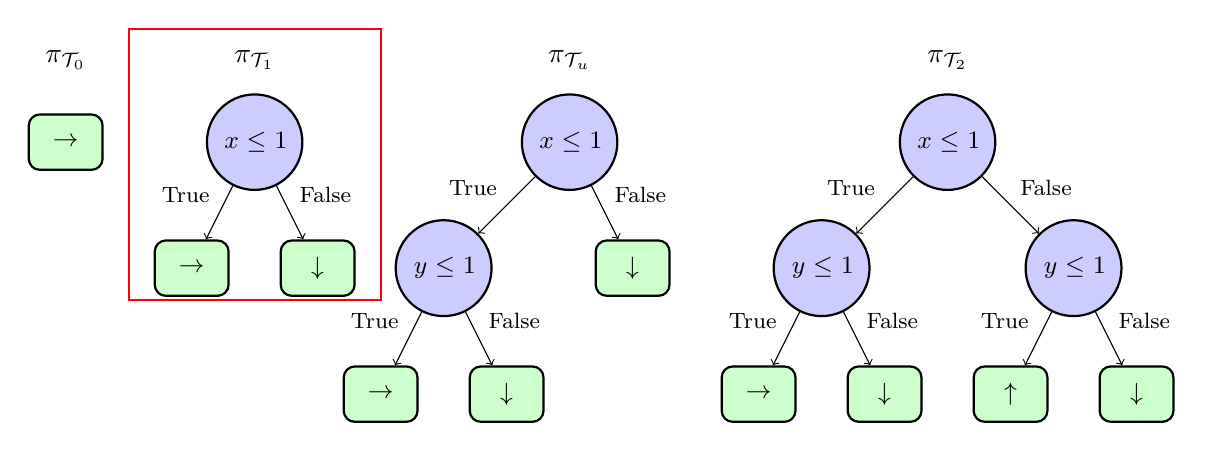
\begin{tikzpicture}[
        scale=0.8,
        decision/.style={circle, draw, thick, fill=blue!20, text width=2.5em, text centered, minimum height=2.5em, font=\small},
        leaf/.style={rectangle, draw, thick, fill=green!20, text width=2em, text centered, rounded corners, minimum height=2em, font=\small},
        edge_label/.style={font=\footnotesize, midway}
    ]
        
        \node[leaf] at (-3, 0) {$\rightarrow$};
        % Tree 4: if x <= 0.5 move right else move left
        \node[decision] (tree4_root) at (0,0) {$x \leq 1$};
        \node[leaf] (tree4_right) at (-1,-2) {$\rightarrow$};
        \node[leaf] (tree4_left) at (1,-2) {$\downarrow$};
        \draw[->] (tree4_root) -- (tree4_right) node[edge_label, above left] {True};
        \draw[->] (tree4_root) -- (tree4_left) node[edge_label, above right] {False};
        
        % Draw a square around the tree
        \draw[thick, red] (-2, 1.8) rectangle (2, -2.5);

        % Tree 7: if x <= 0.5 and y <= 0.5 move right else move down
        \node[decision] (tree7_root) at (5,0) {$x \leq 1$};
        \node[decision] (tree7_y) at (3,-2) {$y \leq 1$};
        \node[leaf] (tree7_right) at (2,-4) {$\rightarrow$};
        \node[leaf] (tree7_down) at (4,-4) {$\downarrow$};
        \node[leaf] (tree7_down2) at (6,-2) {$\downarrow$};
        \draw[->] (tree7_root) -- (tree7_y) node[edge_label, above left] {True};
        \draw[->] (tree7_root) -- (tree7_down2) node[edge_label, above right] {False};
        \draw[->] (tree7_y) -- (tree7_right) node[edge_label, above left] {True};
        \draw[->] (tree7_y) -- (tree7_down) node[edge_label, above right] {False};


        \node[decision] (tree7_root) at (11,0) {$x \leq 1$};
        \node[decision] (tree7_y) at (9,-2) {$y \leq 1$};
        \node[decision] (tree7_y2) at (13,-2) {$y \leq 1$};
        \node[leaf] (tree7_right) at (8,-4) {$\rightarrow$};
        \node[leaf] (tree7_down) at (10,-4) {$\downarrow$};
        \node[leaf] (tree7_right2) at (12,-4) {$\uparrow$};
        \node[leaf] (tree7_down2) at (14,-4) {$\downarrow$};
        \draw[->] (tree7_root) -- (tree7_y) node[edge_label, above left] {True};
        \draw[->] (tree7_root) -- (tree7_y2) node[edge_label, above right] {False};
        \draw[->] (tree7_y) -- (tree7_right) node[edge_label, above left] {True};
        \draw[->] (tree7_y) -- (tree7_down) node[edge_label, above right] {False};
        \draw[->] (tree7_y2) -- (tree7_right2) node[edge_label, above left] {True};
        \draw[->] (tree7_y2) -- (tree7_down2) node[edge_label, above right] {False};

        % Labels
        \node[above] at (-3,1) {$\pi_{\mathcal{T}_0}$};
        \node[above] at (0,1) {$\pi_{\mathcal{T}_1}$};
        \node[above] at (5,1) {$\pi_{\mathcal{T}_u}$};
        \node[above] at (11,1) {$\pi_{\mathcal{T}_2}$};


    \end{tikzpicture}
    \caption{For each decision tree structure, e.g., depth-1 or unbalanced depth-2, we illustrate a decision tree which maximizes the RL objective (\ref{def:mdp-obj}) in the grid world MDP.}
    \label{fig:optimal-policy-trees}
\end{figure}

Because we know all the base states, all the observations, all the actions, all the rewards and all the transitions of our POIBMDP (cf. example~\ref{example:ibmdp}), we can compute exactly the values of different deterministic partially observable policies given, $\zeta$ the reward for IGAs, and $\gamma$ the discount factor.
Each of those policies can be one of the trees illustrated in figure~\ref{fig:optimal-policy-trees}: 

\begin{itemize}
    \item $\pi_{\mathcal{T}_0}$: a depth-0 tree equivalent to always taking the same base action 
    \item $\pi_{\mathcal{T}_1}$: a depth-1 tree equivalent alternating between an IGA and a base action 
    \item $\pi_{\mathcal{T}_u}$: an unbalanced depth-2 tree that sometimes takes two IGAs then a base action and sometimes a an IGA then a base action
    \item $\pi_{\mathcal{T}_2}$: a depth-2 tree that alternates between taking two IGAs and a base action
    \item an inifinite ``tree'' that only takes IGAs
\end{itemize}
Furthermore, because from~\cite{learning-pomdp} we know that for POMDPs, stochastic partially observable policies can sometimes get better expected discounted rewards than deterministic partially observable policies, we also compute the value of the stochastic policy that randomly alternates between two base actions: $\rightarrow$ and $\downarrow$.
Those two base actions always lead to the goal state (cf. figure~\ref{example:grid}).

\begin{proposition}[Depth-1 decision tree objective value] The interpretable RL objective value (\ref{def:irl}) of depth-1 decision tree policies with good interpretability–performance trade-offs in the grid world MDP (cf. figures~\ref{fig:trees-intro} and~\ref{fig:optimal-policy-trees}) is $\frac{4\zeta + \gamma + 2\gamma^3 + \gamma^5}{4(1-\gamma^2)}$.
\end{proposition}

We defer the lengthy proofs of this proposition, as well as the interpretable RL objective values of other decision tree policies, to the appendix~\ref{calcs}.

\begin{figure}
    \centering
    \includegraphics[width=0.6\textwidth]{images/images_part1/objective_values_plot.pdf}
    \caption{Interpretable RL objective values (\ref{def:irl}) of different partially observable policies as functions of $\zeta$. Shaded areas show the optimal \textit{deterministic} partially observable policies in different ranges of $\zeta$ values.}\label{fig:objectives}
\end{figure}

We can now plot, in figure~\ref{fig:objectives}, the interpretable RL objective values of the different partially observable policies as functions of $\zeta$ when we fix $\gamma=0.99$. 
When $\gamma=0.99$ on figure~\ref{fig:objectives}, despite objective values being very similar for the depth-1 and unbalanced depth-2 tree, we now know from the green shaded area that a depth-1 tree is the optimal, w.r.t. the interpretable RL objective, deterministic partially observable POIBMDP policy for $0< \zeta < 1$.

Let us now define a POIBMDP with the grid wolrd (\ref{example:grid}) as the base MDP, with IGAs as in the IBMDP from exapmle~\ref{example:ibmdp}, with $\gamma=0.99$ and $0<\zeta<1$ and verify if RL can retrieve the optimal deterministic partially observable policies w.r.t. the interpretable RL objective, which are equivalent to depth-1 decision tree policies, in this very controlled experiment.

\subsection{Reinforcement learning in PO(IB)MDPs}

In general, the policy that maximizes the RL objective (\ref{def:mdp-obj}) in a POMDP (cf. definition~\ref{def:pomdp}), maps ``belief states'' or observations histories~\cite{chap2} to actions, i.e., those policies are not solutions to our problem since we require that policies depend only on the current observation.
If we did not have this constraint, we could apply any standard RL algorithm to solve POIBMDPs by seeking such policies because both histories and belief states are sufficient statistic for POMDPs hidden states~\cite{chap2,lambrechts2025informed}.

In particular, the problem of finding the optimal deterministic partially observable policies for POMDPs is NP-HARD, even with full knowledge of transitions and rewards~\cite[section 3.2]{littman1}. 

It means that, there is no reason to believe that we have to enumerate all possible policies and take the best one. 
For even moderate-sized POMDPs, a brute-force approach will take a very long time since there are $|A|^{|O|}$ deterministic partially observable policies.

Hence it is interesting to study reinforcement learning for finding the best deterministic partially observable policy since it would not search the whole solution space.
However applying RL to our interpretable RL objective (\ref{def:irl}) is non-trivial.

In~\cite[Fact 2]{learning-pomdp}, authors show that the optimal partially observable policy can be stochastic, hence policy gradient algoriothms~\cite{pg_sutton} are to avoid since we want a \textit{deterministic} policy. 
Furthermore, the optimal deterministic patially observable policy might not maximize all the values of all observations simulataneously ~\cite[Fact 5]{learning-pomdp} which makes it difficult to use TD-learning (cf. algorithms~\ref{alg:qlearning} and~\ref{alg:sarsa}).
Indeed, doing a TD-learning update of one partially observable value~\ref{def:vpo} with, e.g. Q-learning, can change the value of \textit{all} other observations in an uncontrollable manner because of the depedence in $P^{\pi}((s, \boldsymbol{o}')|\boldsymbol{o})$.
Interestingly, those two challenges of learning in POMDPs described in \cite{learning-pomdp} are visible in figure~\ref{fig:objectives}. 
First, there is a whole range of $\zeta$ values for which the optimal partially observable policy is stochastic.
Second, for e.g. $\zeta=0.5$, while a depth-1 tree is the optimal deterministic partially observable policy, the value of state $(\boldsymbol{s}_2, \boldsymbol{o}_0) = (1.5, 1.5, 0, 2, 0, 2)$ is not maximized by this partially observable policy but by the sub-optimal policy that always goes down.

Despite those hardness results, empirical results of applying RL to POMDPs by naively replacing $\boldsymbol{x}$ by $\boldsymbol{o}$ in Q-learning or Sarsa, has already demonstrated successful in practice~\cite{sarsa-pomdp}. 
More recently, the framework of Baisero et. al. called asymmetric RL~\cite{baisero-dqn,baisero-ppo} has also shown promising results to learn POMDP solutions.
Asymmetric RL trains a model depending on hidden states (only available at train time) and a history-dependent (or observation-dependent) model informed by the former.
The history-dependent (or observation-dependent) model can thus be deployed in the POMDP after training since it does not require access to the hidden state to output actions.
In algorithms~\ref{alg:asymqlearning} and~\ref{alg:asymsarsa} we present asymmetric Q-learning and asymmetric Sarsa. Given a POMDP, both train a partially observable Q-function $Q:O\times A\rightarrow\mathbb{R}$ and a Q-function $U:X\times A\rightarrow\mathbb{R}$.

In~\cite{jsj}, authors introduce a policy search algorithm~\ref{sec:rl} that learns a (stochastic) policy $\pi:O\rightarrow\Delta(A)$ and a critic $V:X\rightarrow \mathbb{R}$ using Monte Carlo estimates to guide policy improvement.
We write this algorithm that we call JSJ (for the authors names Jaakkola, Singh, Jordan) in algorithm~\ref{alg:jsj}. JSJ is equivalent to a tabular asymmetric policy gradient algorithm (cf. algorithm~\ref{alg:reinforce}). 

Until recently, the benefits of asymmetric RL over standard RL was only shown empirically and only for history-dependent models.
The work of Gaspard Lambrechts~\cite{justif-asym} proves that some asymmetric RL algorithms learn better history-dependent \textbf{or} partially observable policies for solving POMDPs.
This is exactly what we wish for. However, those algorithms are not practical because they require estimation of the asymptotic occupacy distribution $P^{\pi}((s, \boldsymbol{o}')|\boldsymbol{o})$ (\ref{def:vpo}) for candidate policies which in turn would require to gather a lot of on-policy samples.
We leave it to future work to use those algorithms that combine asymmetric RL and estimation of future visitations since those results are contemporary to the writing of this manuscript.

Note that, in the previous chapter, modified DQN (cf. algorithm~\ref{alg:mod-dqn}) and modified PPO (cf. algorithm~\ref{alg:mod-ppo}) are respectively asymmetric DQN and asymmetric PPO from~\cite{baisero-dqn,baisero-ppo}.
In the next section, we use (asymmetric) RL to optimize the interpretgable RL objective in POIBMDPs.
\RestyleAlgo{ruled}
\SetKwComment{Comment}{}{}
\begin{algorithm}
    \KwData{POMDP $\mathcal{M}_{po} = \langle X, O, A, R, T, T_0, \Omega \rangle$, learning rates $\alpha_u,\quad \alpha_q$, exploration rate $\epsilon$}
    \KwResult{$\pi:O\rightarrow A$}
    Initialize $U(\boldsymbol{x},a) = 0$ for all $x \in X, a \in A$ \\
    Initialize $Q(\boldsymbol{o},a) = 0$ for all $o \in O, a \in A$ \\

    \For{each episode}{
        Initialize state $x_0 \sim T_0$ \\
        Initialize observation $\boldsymbol{o}_0 \sim \Omega(\boldsymbol{x}_0)$ \\

        \For{each step $t$}{
            Choose action $a_t$ using $\epsilon$-greedy: $a_t = \operatorname{argmax}_a Q(\boldsymbol{o}_t,a)$ with prob. $1-\epsilon$ \\
            Take action $a_t$, observe $r_t = R(\boldsymbol{x}_t,a_t)$, $x_{t+1} \sim T(x_t,a_t)$, and $\boldsymbol{o}_{t+1} \sim \Omega(\boldsymbol{x}_{t+1})$ \\
            $y \leftarrow r + \gamma U(\boldsymbol{x}_{t+1}, \operatorname{argmax}_{a'} Q(\boldsymbol{o}_{t+1}, a'))$ \Comment{// TD target} \\
            $U(\boldsymbol{x}_t,a_t) \leftarrow (1 - \alpha_u) U(\boldsymbol{x}_t, a_t) + \alpha_u y $ \\
            $Q(\boldsymbol{o}_t,a_t) \leftarrow (1 - \alpha_q) Q(\boldsymbol{o}_t, a_t) + \alpha_q y $ \\
            $x_t \leftarrow \boldsymbol{x}_{t+1}$ \\
            $\boldsymbol{o}_t \leftarrow \boldsymbol{o}_{t+1}$ \\
        }
    }
    $\pi(o) = \operatorname{argmax}_a Q(\boldsymbol{o},a)$ \Comment{// Extract greedy policy}
    \caption{Asymmetric Q-Learning}\label{alg:asymqlearning}
\end{algorithm}


\RestyleAlgo{ruled}
\SetKwComment{Comment}{}{}
\begin{algorithm}
    \KwData{POMDP $\mathcal{M}_{po} = \langle X, O, A, R, T, T_0, \Omega \rangle$, learning rates $\alpha_u,\quad \alpha_q$, exploration rate $\epsilon$}
    \KwResult{$\pi:O\rightarrow A$}
    Initialize $U(x,a) = 0$ for all $x \in X, a \in A$ \\
    Initialize $Q(o,a) = 0$ for all $o \in O, a \in A$ \\

    \For{each episode}{
        Initialize state $x_0 \sim T_0$ \\
        Initialize observation $\boldsymbol{o}_0 \sim \Omega(x_0)$ \\
        Choose action $a_0$ using $\epsilon$-greedy: $a_0 = \operatorname{argmax}_a Q(\boldsymbol{o}_0,a)$ with prob. $1-\epsilon$ \\

        \For{each step $t$}{
            Take action $a_t$, observe $r_t = R(x_t,a_t)$, $x_{t+1} \sim T(x_t,a_t)$, and $\boldsymbol{o}_{t+1} \sim \Omega(x_{t+1})$ \\
            Choose action $a_{t+1}$ using $\epsilon$-greedy: $a_{t+1} = \operatorname{argmax}_a Q(\boldsymbol{o}_{t+1},a)$ with prob. $1-\epsilon$ \\
            $y \leftarrow r + \gamma U(x_{t+1}, a_{t+1})$ \Comment{// TD target using actual next action} \\
            $U(x_t,a_t) \leftarrow (1 - \alpha_u) U(x_t, a_t) + \alpha_u y $ \\
            $Q(\boldsymbol{o}_t,a_t) \leftarrow (1 - \alpha_q) Q(\boldsymbol{o}_t, a_t) + \alpha_q y $ \\
            $x_t \leftarrow x_{t+1}$ \\
            $\boldsymbol{o}_t \leftarrow \boldsymbol{o}_{t+1}$ \\
            $a_t \leftarrow a_{t+1}$ \\
        }
    }
    $\pi(b\oldsymbol{o}) = \operatorname{argmax}_a Q(\boldsymbol{o},a)$ \Comment{// Extract greedy policy}
    \caption{Asymmetric Sarsa}\label{alg:asymsarsa}
\end{algorithm}

\RestyleAlgo{ruled}
\SetKwComment{Comment}{}{}
\begin{algorithm}
    \KwData{POMDP $\mathcal{M}_{po} = \langle X, O, A, R, T, T_0, \Omega \rangle$, learning rate $\alpha$, policy parameters $\theta$, number of trajectories $N$}
    \KwResult{Stochastic partially observable policy $\pi_\theta: O\rightarrow \Delta(A)$}
    Initialize policy parameters $\theta$ \\
    Initialize $Q(\boldsymbol{o}, a) = 0$ for all observations $o$ and actions $a$ \\
    \For{each episode}{
        \For{$i = 1$ to $N$}{
            Generate trajectory $\tau_i = (\boldsymbol{s}_0, a_0, r_0, \boldsymbol{s}_1, a_1, r_1, \ldots, \boldsymbol{s}_T)$ following $\pi_\theta$ \\
            \For{each timestep $t$ in trajectory $\tau_i$}{
                $G_t \leftarrow \sum_{k=t}^{T} \gamma^{k-t} r_k$ \Comment{// Compute return}
                Store $(\boldsymbol{o}_t, a_t, G_t)$ for later averaging
            }
        }
        \For{each unique observation-action pair $(o, a)$}{
            $Q(o, a) \leftarrow \frac{1}{|\{(\boldsymbol{o}, a)\}|} \sum_{(\boldsymbol{o}, a, G)} G$ \Comment{// Monte Carlo estimate}
        }
        \For{each observation $o$}{
            \For{each action $a$}{
                $\pi_1(a|\boldsymbol{o}) \leftarrow 1.0$ if $a = \operatorname{argmax}_{a'} Q(\boldsymbol{o}, a')$, $0.0$ otherwise \Comment{// Deterministic policy from Q-values}
                $\pi(a|\boldsymbol{o}) \leftarrow (1 - \alpha) \pi(a|\boldsymbol{o}) + \alpha \pi_1(a|\boldsymbol{o}o)$ \Comment{// Policy improvement step}
            }
        }
        Reset $Q(\boldsymbol{o}, a) = 0$ for all observations $\boldsymbol{o}$ and actions $a$ \Comment{// Reset for next episode}
    }
    \caption{JSJ algorithm. Uses Monte Carlo estimates of the average reawrd value functions to perform policy imporvements}\label{alg:jsj}
\end{algorithm}

\section{Results}

Unfortunately, our results are negative and show that (asymmetric) reinforcement learning fails for the aforementioned problem. Let us understand why.

\subsection{Experimental setup}

\paragraph{Baselines:} we consider two groups of RL algorithms.
The first group is standard tabular RL algorithms to optimize the interpretable RL objective in POIBMDPs; Q-learning, Sarsa, and Policy Gradient with a softmax policy (cf. section~\ref{sec:rl}).
In theory the Policy Gradient algorithm should not be a good candidate for our problem since it searches for stochastic policies that we showed can be better than our seeked depth-1 decision tree policy (cf. figure~\ref{fig:objectives}).

In addition to the traditional tabular RL algorithms above, we also apply asymmetric Q-learning, asymmetric Sarsa, and JSJ (algorithms~\ref{alg:asymqlearning},~\ref{alg:asymsarsa} and~\ref{alg:jsj}).
We use at least 200 000 POIBMDP time steps per experiment. Each experiment, i.e an RL algorithm learning in a POIBMDP, is repeated 100 times.  

\paragraph{Hyperparameters:} For all baselines we use, when applicable, exploration rates $\epsilon=0.3$ and learning rates $\alpha=0.1$.

\paragraph{Metrics:} We will consider two metrics.
First, the sub-optimality gap during training, w.r.t. the interpretable RL objective, between the learned partially observable policy and the optimal deterministic partially observable policy: $|\mathbb{E}\left[V^\pi^{\star}(\boldsymbol{s}_0,\boldsymbol{o}_0)| \boldsymbol{s}_0\sim T_0\right] - \mathbb{E}\left[V^\pi(\boldsymbol{s}_0,\boldsymbol{o}_0)|\boldsymbol{s}_0\sim T_0\right]|$.
Because we know the whole POIBMDP model that we can represent exactly as tables; and because we know for each $\zeta$ the interpretable RL objective value of the optimal deterministic partially observable policy (cf. figure); we can report the \textit{exact} sub-optimality gaps.

Second, we consider the distribution of the learned trees over the 100 training seeds.
Indeed, since for every POIBMDP we run each algorihtm 100 times, at the end of training we get 100 deterministic partially observable policies (we compute the greedy policy for stochastic policies returned by JSJ and Policy Gradient), from which we can extract the equivalent 100 decision tree policies using algorithm~\ref{alg:extract-tree} and we can count which one are of e.g. depth-1.
This helps understand which trees RL algorithms tend to learn.

\subsection{Can (asymmetric) RL retrieve optimal deterministic partially observable POIBMDP policies?}

In figure~\ref{fig:rl-poibmdp}, we plot the sub-optimality gaps--averaged over 100 seeds--of learned policies during training.
We do so for 200 different POIBMDPs where we change the reward for information gathering actions: we sample 200 $\zeta$ values uniformily in $[-1, 2]$.
In figure~\ref{fig:rl-poibmdp}, a different color represents a different POIBMDP.

Recall from figure~\ref{fig:objectives} that for:
\begin{itemize}
    \item $\zeta\in [-1, 0]$, the optimal deterministic partially observable policy is a depth-0 tree
    \item $\zeta\in ]0, 1[$, the optimal deterministic partially observable is a depth-1 tree
    \item $\zeta\in [1, 2]$, the optimal deterministic partially observable is a ``inifnite'' tree that contains infinite number of internal nodes.
\end{itemize}
We observe that, despite all sub-optimaility gaps converging, independently of the $\zeta$ values, not all algorithms in all POIBMDPs fully minimize the sub-optimality gap.
In particular, all algorithms seem to consistantly minimze the gap, i.e. learn the optimal policy or Q-function, only for $\zeta \in [1, 2]$ (all the yellow lines go to 0).
However, we are interested in the range $\zeta\in ]0, 1[$ where the optimal decision tree policy is non-trivial, i.e. not taking the same action forever.
In that range, no baseline consistently minimizes the sub-optimality gap.


In figure~\ref{fig:dt-distrib-poibmdp}, we plot the distributions over the final learned trees in function of $\zeta$ from the above runs.
For example, in figure~\ref{fig:dt-distrib-poibmdp}, in the top left plot, when learning 100 times in a POIBMP with $\zeta=0.5$, Q-learning returned almost 100 times a depth-0 tree.
Again, on none of those subplots do we see a high rate of learned depth-1 trees for $\zeta\in ]0, 1[$.
It is alerting that the most frequent learned trees are the depth-0 trees for $\zeta\in ]0, 1[$ because such trees are way more sub-optimal w.r.t. the interpretable RL objective (\ref{def:irl}) than e.g. the depth-2 unbalanced trees (cf. figure~\ref{fig:objectives}).  
One interpretation of this phenomenon is that the learning in POIBMDPs is very difficult and so agents tend to converge to trivial policies, e.g., repeating the same base action.

However, on the positive side, we observe that asymmetric versions of Q-learning and Sarsa have found the optimal deterministic partially observable policy--the depth-1 decision tree--more frequently throughout the optimality range $]0,1[$, than their symmetric counter-parts for $\zeta\in ]0, 1[$.
Next, we quantify how difficult it is to do RL to learn partially observable policies in POIBMDPs.

\begin{figure}
    \centering
    \includegraphics[width=1\textwidth]{images/images_part1/learning_curves.pdf}
    \caption{(Asymmetric) reinforcement learning in POIBMDPs. 
    In each subplot, each single line is colored by the value of $\zeta$ in the corresponding POIBMDP in which learning occurs. 
    Each single learning curve represent the sub-optimality gap averaged over 100 seeds.
    }\label{fig:rl-poibmdp}
\end{figure}

\begin{figure}
    \centering
    \includegraphics[width=1\textwidth]{images/images_part1/tree_distributions.pdf}
    \caption{Distributions of final tree policies learned across the 100 seeds.
    For each $\zeta$ value, there are four colored points. Each point represent the share of depth-0 trees (red), depth-1 trees (green), unbalanced depth-2 trees (orange) and depth-2 trees (blue).
    }\label{fig:dt-distrib-poibmdp}
\end{figure}


\subsection{How difficult is it to learn in POIBMDPs?}\label{sec:how-diff}

In this section we run the same (asymmetric) reinforcement learning algorithms to optimize either the RL objective (\ref{def:mdp-obj}) in MDPs (\ref{def:mdp}) or IBMDPs (\ref{def:ibmdp}), or the interpretable RL objective in POIBMDPs~\ref{def:irl}.
This essentially results in three disctint problems:
\begin{enumerate}
    \item Learning an optimal standard Markovian policy in an MDP, i.e. optimizing the RL objective in an MDP.
    \item Learning an optimal standard Markovian policy in an IBMDP, i.e. optimizing the RL objective in an IBMDP.
    \item Learning an optimal deterministic partially observable policy in a POIBMDP.
\end{enumerate}

In order to see how difficult each of these three problems is, we can run a \textit{great} number of experiments on each and compare success rates.
To make success rates comparable we consider a unique instance for each of those problems.
Problem 1 is, learning one of the optimal standard Markovian deterministic policy from figure~\ref{example:grid} for the grid world from example~\ref{example:grid} with $\gamma=0.99$.
Problem 2 is, learning one of the optimal standard Markovian deterministic for the IBMDP from figure~\ref{example:ibmdp} with $\gamma=0.99$ and $\zeta=0.5$.
This is similar to the previous chapter's experiments where we applied DQN or PPO to an IBMDP for CartPole without constraining the search to partially observable policies (see e.g. figure\ref{fig:res-ppo}).
Problem 3 is, what has been done in the previous section to learn deterministic partially observable policies where in addition of fixing $\gamma=0.99$ we also fix $\zeta=0.5$.

We use the six (asymmetric) RL algoroithms from the previous section and try a wide set of hyperparameters and additional learning tricks (optimistic Q-function, eligibility traces, entropy regularization and $\epsilon$-decay, all are described in \cite{sutton}).
We only provide the detailed hyperparameters for asymmetric Sarsa and an overall summary for all the algorithms in tables~\ref{tab:hp-sarsa} and~\ref{tab:ib-params}.
The complete detailed lists of hyperparameters are given in the appendix~\ref{sec:hp-pomdp}.
Furhtermore, the careful reader might notice that there is no point running asymmetric RL on MDPs or IBMDPs when the problem does not require partial observability.
Hence, we only run asymmetric RL for POIBMDPs and otherwise run all other RL algorithms and all problems.

Each unique hyperparameters combination for a given algorithm on a given problem is run 10 times on 1 million learning steps.
For example, for asymmetric Sarsa, we run a total of $10\times 768= 7680$ experiments for learning deterministic partially observable policies for a POIBMDP (cf. table~\ref{tab:hp-sarsa}).
To get a success rate, we can simply divide the number of learned depth 1 tree by 7680 (recall that for $\gamma=0.99$ and $\zeta=0.5$, the optimal policy is a depth-1 tree (e.g. figure~\ref{fig:optimal-policy-trees}) as per figure~\ref{fig:objectives}). 

\begin{table}
\centering
\small
\caption{Asymmetric sarsa hyperparameters (768 combinations each run 10 times)}\label{tab:hp-sarsa}
\begin{tabular}{lll}
\toprule
\textbf{Hyperparameter} & \textbf{Values} & \textbf{Description} \\
\midrule
Epsilon Schedules & (0.3, 1), (0.3, 0.99), (1, 1) & Initial exploration and decrease rate \\
Epsilon Schedules & (0.1, 1), (0.1, 0.99), (0.3, 0.99) & Initial exploration and decrease rate \\
Lambda & 0.0, 0.3, 0.6, 0.9 & Eligibility trace decay \\
Learning Rate $U$ & 0.001, 0.005, 0.01, 0.1 & learning rate for \\
 & & the Q-function \\
Learning Rate $Q$ & 0.001, 0.005, 0.01, 0.1 & learning rate for the \\
 & & partial observation dependent Q-function \\
Optimistic & True, False & Optimistic initialization \\
\bottomrule
\end{tabular}
\end{table}

\begin{table}
    \centering
    \caption{Summary of RL baselines Hyperparameters}\label{tab:ib-params}
    \begin{tabular}{llr}
    \toprule
    \textbf{algorithm} & \textbf{Problem} & \textbf{Total Hyperparameter Combinations} \\
    \midrule
    Policy Gradient & PO/IB/MDP & 420 \\
    JSJ & POIBMDP & 15 \\
    Q-learning & PO/IB/MDP & 192 \\
    Asym Q-learning & POIBMDP & 768 \\
    Sarsa & PO/IB/MDP & 192 \\
    Asym Sarsa & POIBMDP & 768 \\
    \bottomrule
    \end{tabular}
    \end{table}


The key observations from figure~\ref{fig:po-vs-ib} is that reinforcement learning a deterministic partially observable policy in a POIBMDP, is way harder than learning Q-function of policies that have access to all the state information.
For example, Q-learning only finds the optimal solution to (\ref{def:irl}) in only 3\% of the experiments while the same algorithms to optimize the standard RL objective (\ref{def:mdp-obj}) in an MDP or IBMDP found the optimal solutions 50\% of the time.
Even though asymmetry seems to increase performances; learning a decision tree policy for a simple grid world directly with RL using the framework of POIBMDP originally developed in~\cite{topin2021iterative} seems way too difficult and costly as successes might require a million steps for such a seemingly simple problem.
An other difficulty in practice that we did not cover here, is the choice of information gathering actions.
For the grid world MDP, choosing good IGAs ($x\leq1$ and $y\leq1$) is simple but what about more complicated MDPs: how to instantiate the (PO)IBMDP action space such that internal nodes in resulting trees are useful for predictions?

To go even further, on figure~\ref{fig:asym-ql-analysis} we re-run experiments from figure~\ref{fig:rl-poibmdp} and figure~\ref{fig:dt-distrib-poibmdp} using the top performing hyperparameters for asymmetric Q-learning (given in appendix~\ref{tab:algorithm-hyperparameters}).
While those hyperparemeters resulted in asymmetric Q-learning returning 10 of out 10 times an optimal depth 1 tree,
the performances didn't transfer.
On figure~\ref{fig:asym-ql-analysis} depsite higher success rates in the region $\zeta\in]0,1[$ compared to figure~\ref{fig:dt-distrib-poibmdp}. 

\begin{figure}
    \centering
    \includegraphics[width=0.8\textwidth]{images/images_part1/algorithm_performance_comparison_flattened.pdf}
    \caption{Success rates of different (asymmetric) RL algorithms over thousands of runs when applied to learning deterministic partially observable policies in a POIBMDP or learning deterministic policies in associated MDP and IBMDP.}\label{fig:po-vs-ib}
\end{figure}


\begin{figure}
    \begin{subfigure}[b]{0.49\textwidth}
        \includegraphics[width=\textwidth]{images/images_part1/ql_asym_best_learning_curves.pdf}
        \caption{Learning curves for asymmetric Q-learning with good hyperparameters.}
        \label{fig:best-learning-curves}
    \end{subfigure}
    \hfill
    \begin{subfigure}[b]{0.49\textwidth}
        \includegraphics[width=\textwidth]{images/images_part1/ql_asym_best_tree_distributions.pdf}
        \caption{Trees distributions for asymmetric Q-learning with good hyperparameters}
        \label{fig:best-tree-distributions}
    \end{subfigure}
    \caption{Analysis of the top-performing asymmetric Q-learning instantiation. (left) Learning curves, and (right) tree distributions across different POIBMDP configurations.}
    \label{fig:asym-ql-analysis}
\end{figure}


\section{Conclusion}
In this chapter, we have shown that direct learning of decision tree policies for MDPs can be reduced to learning deterministic partially observable policies in POMDPs that we called POIBMDPs.
By crafting a POIBMDP for which we know exactly the optimal deterministic partially observable policy w.r.t. the interpretable RL objective (\ref{def:irl}), we were able to benchmark the sub-optimality of solutions learned with (asymmetric) reinforcement learning.

Across our experiments, we found that no algorithm could consistently learn a depth-1 decision tree policy for a grid world MDP despite it being optimal both w.r.t. the interpretable RL objective and standard RL objective (\ref{def:mdp-obj}).
When compared to the results of VIPER in the introductory example~\ref{sec:limits-il}, direct RL is worse at retrieving decision tree policies with good interpretability-performance trade-offs.
This echoes the results from the previous chapter in which we saw that direct deep RL performed worse than imitation learning to find decision tree policies for CartPole.

In the next chapter, we find that RL can find optimal deterministic partially observable policies for a special class of POIBMDPs that we believe makes for a convincing argument as to why direct learning of decision tree policies that optimize the RL objective (\ref{def:mdp-obj}) is so difficult.

\chapter{When transitions are uniform POIBMDPs are fully observable}
\begin{figure}
    \centering
    \includegraphics[width=1\textwidth]{images/images_part1/quick_plot_combined_classif.pdf}
    \caption{RL algorithms for classif OPOIBMDPs}\label{fig:rl-poibmdp}
\end{figure}



\part{An Easier Problem: Decision Tree Induction as Solving MDPs}\label{part2}
\chapter{DPDT-intro}
\begin{figure}
    \includegraphics[width=\textwidth]{images/figures/patho_bounds_comparison_checkers.pdf}
    \caption{Pathological dataset and learned depth-2 trees with their scores, complexities, runtimes, and decision boundaries.}
    \label{fig:patho}
\end{figure}
In supervised learning, decision trees are valued for their interpretability and performance. 
While greedy decision tree algorithms like CART remain widely used due to their computational efficiency, they often produce sub-optimal solutions with respect to a regularized training loss. 
Conversely, optimal decision tree methods can find better solutions but are computationally intensive and typically limited to shallow trees or binary features. We present Dynamic Programming Decision Trees (DPDT), a framework that bridges the gap between greedy and optimal approaches. 
DPDT relies on a Markov Decision Process formulation combined with heuristic split generation to construct near-optimal decision trees with significantly reduced computational complexity. 
Our approach dynamically limits the set of admissible splits at each node while directly optimizing the tree regularized training loss. Theoretical analysis demonstrates that DPDT can minimize regularized training losses at least as well as CART\@. 
Our empirical study shows on multiple datasets that DPDT achieves near-optimal loss with orders of magnitude fewer operations than existing optimal solvers. 
More importantly, extensive benchmarking suggests statistically significant improvements of DPDT over both CART and optimal decision trees in terms of generalization to unseen data. We demonstrate DPDT practicality through applications to boosting, where it consistently outperforms baselines. 
Our framework provides a promising direction for developing efficient, near-optimal decision tree algorithms that scale to practical applications.

\section{Introduction}
Decision trees~\cite{ID3,c45,breiman1984classification} are at the core of various machine learning applications. 
Ensembles of decision trees such as tree boosting~\cite{stcohFriedman,FriedmanBoosting,xgb,10.5555/3327757.3327770} are the state-of-the-art for supervised learning on tabular data \cite{grinsztajn2022tree}.
Human users can make sense of decision trees predictions~\cite{rigourous,lipton,pmlr-v247-bressan24a} which allows for real-world applications when safety or trust is critical \cite{saux:hal-04192198}. 
More recently, decision trees have been used to model sequential decision policies with imitation learning~\cite{viper,kohler2024interpretable} or directly with reinforcement learning (RL) \cite{topin2021iterative,vos2024optimizinginterpretabledecisiontree,mdpdt,marton2024sympolsymbolictreebasedonpolicy}.

To motivate the design of new decision tree induction algorithms, Figure~\ref{fig:patho} exhibits a dataset for which existing greedy algorithms are suboptimal, and optimal algorithms are computationally expensive. 
The dataset is made up of $N=10^4$ samples in $p=2$ dimensions that can be perfectly labeled with a decision tree of depth 2. When running CART \cite{breiman1984classification}, greedily choosing the root node yields a suboptimal tree.
This is because greedy algorithms compute locally optimal splits in terms of information gain. In our example, the greedy splits always give two children datasets which themselves need depth 2 trees to be perfectly split.
On the other hand, to find the root node, an optimal algorithm such as \cite{quantbnb} iterates over all possible splits, that is, $N\times p=\numprint{20,000}$ operations to find one node of the solution tree.

In this work, we present a framework for designing non-greedy decision tree induction algorithms that optimize a regularized training loss nearly as well as optimal methods. This is achieved with orders of magnitude less operations, and hence dramatic computation savings.
We call this framework ``Dynamic Programming Decision Trees'' (DPDT). For every node, DPDT heuristically and dynamically limits the set of admissible splits to a few good candidates. Then, DPDT optimizes the regularized training loss with some depth constraints.
Theoretically, we show that DPDT minimizes the empirical risk at least as well as CART\@.
Empirically, we show that on all tested datasets, DPDT can reach 99\% of the optimal regularized train accuracy while using thousands times less operations than current optimal solvers. 
More importantly, we follow \cite{grinsztajn2022tree} methodology to benchmark DPDT against both CART and optimal trees on hard datasets. Following the same methodology, we compare boosted DPDT \cite{FREUND1997119} to boosted CART and to some deep learning methods and show clear superiority of DPDT.

\section{Related Work}

To learn decision trees, greedy approaches like CART \cite{breiman1984classification} iteratively partition the training dataset by taking splits optimizing a local objective such as the Gini impurity or the entropy. 
This makes CART suboptimal with respect to training losses \cite{Murthy}. 
But CART remains the default decision tree algorithm in many machine learning libraries such as \cite{scikit-learn,xgb,ke2017lightgbm,9533597} because it can scale to very deep trees and is very fast.
To avoid overfitting, greedy trees are learned with a maximal depth or pruned a posteriori \cite[chapter~3]{breiman1984classification}. 
In recent years, more complex optimal decision tree induction algorithms have shown consistent gains over CART in terms of generalization capabilities \cite{oct,verwer2017learning,murtree}.

Optimal decision tree approaches optimize a regularized training loss while using a minimal number of splits~\cite{oct,mfoct,binoct,quantbnb,murtree,blossom,pystreed,chaouki2024branchesfastdynamicprogramming}.
However, direct optimization is not a convenient approach, as finding the optimal tree is known to be NP-Hard \cite{npcomplete}. Despite the large number of algorithmic tricks to make optimal decision tree solvers efficient~\cite{murtree,quantbnb}, their complexity scales with the number of samples and the maximum depth constraint.
Furthermore, optimal decision tree induction algorithms are usually constrained to binary-features dataset while CART can deal with any type of feature. When optimal decision tree algorithms deal with continuous features, they can usually learn only shallow trees, e.g. Quant-BnB \cite{quantbnb} can only compute optimal trees up to depth 3.
\texttt{PySTreeD}, the latest optimal decision tree library~\cite{pystreed}, can compute decision trees with depths larger than three but uses heuristics to binarize a dataset with continuous features during a pre-processing step. % following for example the Minimum Description Length Principle \cite{MDL}. 
Despite their limitations to binary features and their huge computational complexities, encouraging practical results for optimal trees have been obtained \cite{how-eff,lin2020generalized,costa2023recent,vanderlinden2024optimalgreedydecisiontrees}.
Among others, they show that optimal methods under the same depth constraint (up to depth four) find
trees with 1--2\% greater test accuracy than greedy methods.


In this work, we only consider the induction of nonparametric binary depth-constrained axis-aligned trees. By nonparametric trees, we mean that we only consider tree induction algorithms that optimize both features and threshold values in internal nodes of the tree. This is different from the line of work on Tree Alternating Optimization (TAO) algorithm~\cite{NEURIPS2018_185c29dc,9534446,10.1145/3412815.3416882} that only optimizes tree nodes threshold values for fixed nodes features similarly to optimizing neural network weights with gradient-based methods. 

There exist many other areas of decision tree research \cite{loh2014fifty} such as inducing non-axis parallel decision trees \cite{murthy1994system,10.1145/3637528.3671903}, splitting criteria of greedy trees \cite{vanderlinden2024optimalgreedydecisiontrees}, different optimization of parametric trees \cite{NIPS2015_1579779b,10.5555/3327757.3327770}, or pruning methods \cite{pruning1,pruning2}. 

Our work is not the first to formulate the decision tree induction problem as solving a Markov decision process (MDP)~\cite{Dulac_Arnold_2011,garlapati2015reinforcementlearningapproachonline,topin2021iterative,chaouki2024branchesfastdynamicprogramming}. Those works formulate tree induction as solving a partially observable MDP and use approximate algorithms such as Q-learning  \cite{garlapati2015reinforcementlearningapproachonline} or deep Q-learning \cite{topin2021iterative} to solve them in an online fashion one datum from the dataset at a time. In a nutshell, our work, DPDT that we present next, is different in that it builds a stochastic and fully observable MDP that can be explicitly solved with dynamic programming. This makes it possible to solve exactly the decision tree induction problem. 


\chapter{Decision tree induction as a solving an MDP}\label{sec:dt-mdp}

\section{The Markov decision process}\label{sec:the-mdp}
We now formulate the decision tree induction problem \ref{eq:suplearning} as finding the optimal policy in an MDP (\ref{def:mdp-obj}).

Given a set of examples $\mathcal{E}$, the induction of a decision tree is made of a sequence of decisions: at each node, we must decide whether it is better to split (a subset of) $\mathcal{E}$, or %assign a class label and 
to create a leaf node.

This sequential decision-making process corresponds to an MDP $\mathcal{M} \langle S, A, R_{\alpha}, T, T_0 \rangle$ (\ref{def:mdp}) that we present next.
%The state space $S$ consists of pairs $(X,d)$ where $X \subseteq \mathcal{E}$, and $d \in \{0,\ldots,D\}$ is the current depth in the tree. Formally $S = \{ (X, d) \in P(\mathcal{E}) \times \{0, \ldots, D\} \}$ where $P(\mathcal{E})$ denotes the power set of $\mathcal{E}$.
A state is a pair made of a subset of examples $\mathcal{X}\subseteq\mathcal E$ and a depth $d$.
Like for classification POIBMDPs (cf. definition~\ref{def:ibmdp} and algorithm~\ref{alg:extract-tree}), the depth $d$ is actually not necessary to extract a tree from a policy.
However, it is necessary in order to solve the MDP.
Indeed, because we constrain the model class to limited-depth trees, the horizon of our MDP is finite and hence as per~\cite{puterman}, the optimal policy is non-Markovian and depends on the time.

The set of states is $S = \{ (\mathcal{X}, d) \in P(\mathcal{E}) \times \{0, \ldots, D\} \}$ where $P(\mathcal{E})$ denotes the power set of $\mathcal{E}$. $d \in \{0,\ldots,D\}$ is the current depth in the tree.
An action $A$ consists in creating either a split node, or a leaf node (label assignment). We denote the set of candidate split nodes $ {\mathcal F} $. A split node in $\mathcal F$ is a pair made of one feature $i$ and a threshold value $x_{ij}\in \mathcal{E}$.
So, we can write $A = {\mathcal{F} \cup \{ 1, \ldots, K \}}$ (these are essentially information gathering actions).
From state $s=(X,d)$ and a splitting action $a \in {\mathcal F}$, the transition function $P$ moves to the next state $s_l = (\mathcal{X}_l, d+1)$ with probability $p_l = \frac{|\mathcal{X}_l|}{|\mathcal{X}|}$ where $\mathcal{X}_l = \{(\boldsymbol{x}_i, y_i) \in \mathcal{X}: \boldsymbol{x}_i \leq x_{ij}\}$, or to state $s_r = (\mathcal{X} \setminus \mathcal{X}_l, d+1)$ with probability $1-p_l$. For a class assignment action $a \in \{1,\ldots,K\}$, the chain reaches an absorbing terminal state with probability 1. 
The reward function $R_{\alpha}: S \times A \rightarrow \mathbb{R}$ returns $-\alpha$ for splitting actions (this is $\zeta$ in a classificaion POIBMDP (\ref{def:cpoibmdp})) and the proportion of misclassified examples of $\mathcal{X}$ $-\frac{1}{|\mathcal{X}|}\sum_{(\boldsymbol{x}_i,y_i) \in \mathcal{X}} l(y_i, a)$ for class assignment actions. $\alpha \in [0,1]$ controls the accuracy-complexity trade-off defined in the regularized training objective \ref{eq:suplearning}. 

The solution to this MDP is a deterministic policy $\pi: S \rightarrow A$ that maximizes {$J_{\alpha}(\pi) ={\mathbb{E}}\left[\sum_{t = 0}^D R_{\alpha}(s_t, \pi(s_t))\right]$\label{def:finite-mdp-obj}}, the expected sum of rewards where the expectation is taken over transitions $s_{t+1}\sim P(s_t, \pi(s_t))$ starting from initial state $s_0 = (\mathcal{E}, 0)$.
This objective is a re-writing of (\ref{def:mdp-obj}) where the trajectory have finite lengths $D$ rather than being infinite.
Any such policy can be converted into a binary decision tree through a recursive extraction function $E(\pi, s)$ (equivalent to algorithm~\ref{alg:extract-tree}) that returns, either a leaf node with class $\pi(s)$ if $\pi(s)$ is a class assignment, or a tree with root node containing split $\pi(s)$ and left/right sub-trees $E(\pi, s_l)$/$E(\pi, s_r)$ if $\pi(s)$ is a split. The final decision tree $T$ is obtained by calling $E(\pi, s_0)$ on the initial state $s_0$. 

\begin{proposition}[Objective Equivalence]\label{prop:equiv}
Let $\pi$ be a deterministic policy of the MDP (\ref{sec:the-mdp}) and $\pi^*$ be an optimal deterministic policy. 
Then $J_\alpha(\pi) = -{\mathcal L}_\alpha(E(\pi, s_0))$ and $T^* = E(\pi^*, s_0)$ where $T^*$ is a tree that optimizes the decision tree induction objective (cf. definition~\ref{eq:suplearning}).
\end{proposition}
This proposition is key as it states that the return of any policy of the MDP defined above is equal to the regularized training accuracy of the tree extracted from this policy.
A consequence of this proposition is that when all possible splits are considered, the optimal policy will generate the optimal tree in the sense defined by (~\eqref{eq:suplearning}).

\begin{proof}
For the purpose of the proof, we overload the definition of $J_\alpha$ and $\mathcal L_\alpha$, to make explicit the dependency on the dataset and the maximum depth. 
As such, $J_\alpha(\pi)$ becomes $J_\alpha(\pi, {\mathcal E}, D)$ and ${\mathcal L}_\alpha(T)$ becomes ${\mathcal L}_\alpha(T, {\mathcal E})$. 
Let us first show that the relation $J_\alpha(\pi, {\mathcal E}, 0) = -{\mathcal L}_\alpha(T, {\mathcal E})$ is true. 
If the maximum depth is $D = 0$ then $\pi(s_0)$ is necessarily a class assignment, in which case the expected number of splits is zero and the relation is obviously true since the reward is the opposite of the average classification loss. 
Now assume it is true for any dataset and tree of depth at most $D$ with $D \geq 0$ and let us prove that it holds for all trees of depth $D + 1$. 
For a tree $T$ of depth $D + 1$ the root is necessarily a split node. Let $T_l = E(\pi, s_l)$ and $T_r = E(\pi, s_r)$ be the left and right sub-trees of the root node of $T$. 
Since both sub-trees are of depth at most $D$, the relation holds and we have $J_\alpha(\pi, \mathcal{X}_l, D) = {\mathcal L}_\alpha(T_l, \mathcal{X}_l)$ and $J_\alpha(\pi, \mathcal{X}_r, D) = {\mathcal L}_\alpha(T_r, \mathcal{X}_r)$, where $\mathcal{X}_l$ and $\mathcal{X}_r$ are the datasets of the ``right'' and ``left'' states to which the MDP transitions---with probabilities $p_l$ and $p_r$---upon application of $\pi(s_0)$ in $s_0$, as described in the MDP formulation. 
Moreover, from the definition of the policy return we have 
\begin{align*}
   J_\alpha(&\pi, {\mathcal E}, D + 1) = -\alpha + p_l * J_\alpha(\pi, \mathcal{X}_l, D) + p_r * J_\alpha(\pi, \mathcal{X}_r, D)\\
   &= -\alpha - p_l * {\mathcal L}_\alpha(T_l, \mathcal{X}_l) - p_r * {\mathcal L}_\alpha(T_r, D)\\
   &= -\alpha - p_l * \Bigg(\frac{1}{|\mathcal{X}_l|}\sum_{(\boldsymbol{x}_i, y_i)\in \mathcal{X}_l}l(y_i, T_l(\boldsymbol{x}_i))  + \alpha C(T_l)\Bigg)\\
   &\ - p_r * \Bigg(\frac{1}{|\mathcal{X}_r|}\sum_{(\boldsymbol{x}_i, y_i)\in \mathcal{X}_r}l(y_i, T_r(\boldsymbol{x}_i))  + \alpha C(T_r)\Bigg)\\
   &= -\frac{1}{N}\sum_{(\boldsymbol{x}_i, y_i)\in \mathcal{X}}l(y_i, T(\boldsymbol{x}_i)) - \alpha (1 + p_l C(T_l) + p_r C(T_r))\\
   &= -{\mathcal L}(T, {\mathcal E}) 
\end{align*}
\end{proof}

\section{Algorithm}\label{sec:dpdt}

We now present the Dynamic Programming Decision Tree (DPDT) induction algorithm. 
The algorithm consists of two essential steps. The first and most computationally expensive step constructs the MDP presented in section~\ref{sec:the-mdp}. 
The second step solves it to obtain a policy that maximizes (\ref{def:finite-mdp-obj}) and that is equivalent to a decision tree. Both steps are now detailed.

\subsection{Constructing the MDP}

An algorithm constructing the MDP of section~\ref{sec:the-mdp} essentially computes the set of all possible decision trees of maximum depth $D$ which decision nodes are in $\mathcal F$. 
The transition function of this specific MDP is a directed acyclic graph. Each node of this graph corresponds to a state for which one computes the transition and reward functions. 
%% PP : je comment-out ce qui suit qui est un détail d'implantation qui ne change rien à la complexité de l'algorithme. Il faut le dire plus loin ; d'ailleurs il en est aussi déjà question en 4.3.
%To limit memory usage of non-terminal nodes, instead of storing all the samples in $(\mathcal{X},d)$, we only store $d$ and the binary vector of size $N$, $x_{bin} = {(1_{\{\boldsymbol{x}_i \in \mathcal{X}\}})}_{i\in \{1,\ldots,N\}}$. 
%Even then,
Considering all possible splits in $\mathcal F$ does not scale.
We thus introduce a state-dependent action space $A_s$, much smaller than $A$ and populated by a splits generating function. In figure \ref{fig:schema-mdp}, we illustrate the MDP constructed for the classification of a toy dataset using some arbitrary splitting function.

\begin{figure}
      \centering
      \includegraphics[width=0.9\linewidth]{images/figures/schema_mdp.pdf}
      \caption{Schematics of the MDP (\ref{sec:the-mdp}) to learn a decision tree of depth 2 to classify a toy dataset with three samples, two features (x,y), and two classes (oval, diamond) and using an arbitrary splits generating function.}\label{fig:schema-mdp}
      \end{figure}

\subsection{Heuristic splits generating functions}\label{sec:testgen}

A split generating function is any function $\phi$ that maps an MDP state, i.e., a subset of training examples, to a split node. It has the form $\phi: S \rightarrow P(\mathcal{F})$, where $P(\mathcal{F})$ is the power set of all possible split nodes in $\mathcal F$. 
For a state $s \in S$, the state-dependent action space is defined by $A_s = \phi(s) \cup  \{1,\ldots,K\}$. 

When the split generating function does not return all the possible candidate split nodes given a state, solving the MDP with state-dependent actions $A_s$ is not guaranteed to yield the minimizing tree of (\ref{eq:suplearning}), as the 
optimization is then performed on the subset of trees of depth smaller or equal to $D$, $\mathcal{T}_D$. 
We now define some interesting split generating functions and provide the time complexity of the associated decision tree algorithms. The time complexity is given in big-O of the number of candidate split nodes considered during computations. 
% Building a depth-1 greedy tree hides a time complexity of $O(np\log(np))$ to sort the splits by information gains \cite{breiman1984classification}.
%%%>>>>>>> c90c7909bd5d3b8cfee3901e21a456980dfd72e1

\paragraph{Exhaustive function} When $\mathcal{F} \subseteq \phi(s), \forall s \in S$, the MDP contains all possible splits of a certain set of examples. In this case, \textit{the optimal MDP policy is the optimal decision tree of depth at most D},
and the number of states of the MDP would be $O({(2Np)}^D)$. Solving the MDP for $A_s = \phi(s)$ is equivalent to running one of the optimal tree induction algorithms~\cite{verwer2017learning,oct,pystreed,quantbnb,binoct,murtree,mfoct,blossom,lin2020generalized,chaouki2024branchesfastdynamicprogramming}

\paragraph{Top $B$ most informative splits}\label{topk-heuristic}~\cite{topk} proposed to generate splits with a function that returns, for any state $s=(\mathcal{X},d)$, the $B$ most informative splits over $\mathcal{X}$ with respect to some information gain measure such as the entropy or the Gini impurity. 
The number of states in the MDP would be $O({(2B)}^D)$. \textit{When $B=1$, the optimal policy of the MDP is the greedy tree.} 
In practice, we noticed that the returned set of splits lacked diversity and often consists of splits on the same feature with minor changes to the threshold value. 

% PP : don't know why mais ci-dessous, si on met un '.' après {CART}, le pdf en affiche 2. Si on n'en met pas, on en voit un !
\paragraph{Calls to CART}\label{cart-heuristic} Instead of returning the most informative split at each state $s=(\mathcal{X},d)$, we propose to find the most discriminative split, i.e.\@ the feature splits that best predicts the class of data in $\mathcal{X}$.
We can do this by considering the split nodes of the greedy tree. In practice, we run CART on $s$ and use the returned nodes as $\phi(s)$. We control the number of MDP states by constraining CART trees with a maximum number of nodes $B$: $\phi(s) = nodes(\text{CART}(s, max\_nodes=B))$
The number of MDP states would be $O({(2B)}^D)$.\textit{When $B=1$, the MDP policy corresponds to the greedy tree.} The process of generating split nodes with calls to CART is illustrated in figure \ref{fig:schema-dpdt}.

\begin{figure}
      \centering
      \includegraphics[trim={0 0cm 0 0},clip,width=0.9\textwidth]{images/figures/schematic_cart_node_select.pdf}
      \caption{How CART is used in DPDT to generate candidate splits given the example data in the current state.}\label{fig:schema-dpdt}
\end{figure}



\subsection{Dynamic programming to solve the MDP}
\RestyleAlgo{ruled}
\SetKwComment{Comment}{}{}
        \begin{algorithm}
            \KwData{$\text{Dataset }\mathcal{E}, \text{max depth }D, \text{split function }\phi(), $\\
            $\text{split function parameter } B,  \text{regularizing term }\alpha$}
            \KwResult{$\text{Tree } T$}
            $\mathcal{M} \gets build\_mdp(\mathcal{E}, D, \phi(), B)$\label{line:build_mdp} \\
            \Comment{{// Backward induction}}
            $Q^*(s,a) \gets R_{\alpha}^{\mathcal{M}}(s,a) + \sum_{s'} P^{\mathcal{M}}(s,a,s') \max_{a' \in A_{s'}^{\mathcal{M}}} Q^*(s',a') \forall s,a \in \mathcal{M}$\\
            \Comment{{// Get the optimal policy}}
            $\pi^*(s) = \operatorname{argmax}_{a \in A_s^{\mathcal{M}}} Q^*(s, a) \forall s \in \mathcal{M} $\\
            \Comment{{// Extracting tree from policy}}
            $T \gets E(\pi^*,s_0^{\mathcal{M}}) $
            \caption{DPDT}\label{alg:dpdt}
        \end{algorithm}
        
After constructing the MDP with a chosen splits generating function, we solve for the optimal policy using dynamic programming. Starting from terminal states and working backward to the initial state, we compute the optimal state-action values using Bellman's optimality equation~\cite{Bellman}, and then deducing the optimal policy.

From now on, we write DPDT to denote algorithm \ref{alg:dpdt} when the split function is a call to CART. We discuss key bottlenecks when implementing DPDT in subsequent sections. We now state theoretical results when using DPDT with the CART heuristic. 

\subsection{Performance guarantees for DPDT}
We now show that: 1) DPDT minimizes the loss from (\ref{eq:suplearning}) at least as well as greedy trees and 2) there exists problems for which DPDT has strictly lower loss than greedy trees. 
As we restrict the action space at a given state $s$ to a subset of all possible split nodes, DPDT is not guaranteed to find the tree minimizing Eq. \ref{eq:suplearning}. However, we are still guaranteed to find trees that are better or equivalent to those induced by CART:
\begin{theorem}[MDP solutions are not worse than the greedy tree]\label{prop:cart}
Let $\pi^*$ be an optimal deterministic policy of the MDP, where the action space at every state is restricted to the top $B$ most informative or discriminative splits. 
Let $T_0$ be the tree induced by CART and $\{T_1,\dots,T_M\}$ all the sub-trees of $T_0$, \footnote{These sub-trees are interesting to consider since they can be returned by common postprocessing operations following a call to CART, that prune some of the nodes from $T_0$. Please see \cite{pruning1} for a review of pruning methods for decision trees.} then for any $\alpha > 0$, 
\[
{\mathcal L}_\alpha(E(\pi^*, s_0)) \leq \min_{0\leq i\leq M}{\mathcal L}_\alpha(T_i)
\]
\end{theorem}

\begin{proof}
Let us first define $C(T)$, the expected number of splits performed by tree $T$ on dataset $\mathcal E$. 
Here $T$ is deduced from policy $\pi$, i.e. $T=E(\pi, s_0)$. $C(T)$ can be defined recursively as $C(T) = 0$ if $T$ is a leaf node, and $C(T) = 1 + p_l C(T_l) + p_r  C(T_r)$, where $T_l = E(\pi, s_l)$ and $T_r = E(\pi, s_r)$. 
In words, when the root of $T$ is a split node, the expected number of splits is one plus the expected number of splits of the left and right sub-trees of the root node.
\end{proof}

It is known that the greedy tree of depth 2 fails to perfectly classify the XOR problem as shown in figure \ref{fig:patho} and in \cite{Murthy,how-eff}. We aim to show that DPDT is a cheap way to alleviate the weaknesses of greedy trees in this type of problems. The following theorem states that there exist classification problems such that DPDT optimizes the regularized training loss strictly better than greedy algorithms such as CART, ID3 or C4.5.
\begin{theorem}[DPDT can be strictly better than greedy]\label{thm:better_greedy}
There exists a dataset and a depth $D$ such that the DPDT tree $T^{DPDT}_D$ is strictly better than the greedy tree $T^{greedy}_{D}$ , i.e, $\mathcal{L}_{\alpha=0}(T^{greedy}_{D}) > \mathcal{L}_{\alpha=0}(T^{DPDT}_{D})$.
\end{theorem}

The proof of this theorem is given in the next section.

\subsection{Proof of improvement over CART}\label{proof-improve-opt}
In this section we construct a dataset for which the greedy tree of depth 2 fails to accurately classify data while DPDT with calls to CART as a splits generating function guarantees a strictly better accuracy. The dataset is the XOR pattern like in figure \ref{fig:patho}. We will first show that greedy tree induction like CART chooses the first split at random and the second split in between the two columns or rows. Then we will quantify the misclassification of the depth-2 greedy tree on the XOR gate. Finally we will show that using the second greedy split as the root of a tree and then building the remaining nodes greedily, i.e. running DPDT with the CART heuristic, strictly decreases the misclassification. 
\begin{definition}[XOR dataset]\label{def:checkerboard}
     Let us defined the XOR dataset as $\mathcal{E}_{XOR} = \{(\boldsymbol{x}_i, y_i)\}_{i=1}^N$. $\boldsymbol{x}_i = (\boldsymbol{x}_i, y_i) \sim \mathcal{U}([0,1]^2)$ are i.i.d 2-features samples. $y_i = f(\boldsymbol{x}_i)$ are alternating classes with $f(x,y) = (\lfloor 2x \rfloor + \lfloor 2y \rfloor) \bmod 2$.
\end{definition}

\begin{lemma} The first greedy split is chosen at random on the XOR dataset from definition \ref{def:checkerboard}.
\end{lemma}\label{lem:first-split}
\begin{proof}
Let us consider an arbitrary split $x = x_v$ parallel to the y-axis. The results apply to splits parallel to the x-axis because the XOR pattern is the same when rotated 90 degrees. The split $x_v$ partitions the dataset into two regions $R_{left}$ and $R_{right}$. Since the dataset has two columns and two rows, any rectangular area that spans the whole height $[0,1)$ has the same proportion of class 0 samples and class 1 samples from definition \ref{def:checkerboard}. So in both $R_{left}$ and $R_{right}$ the probabilities of observing class 0 or class 1 at random are $\frac{1}{2}$. Since the class distributions in left and right regions are independent of the split location, all splits have the same objective value when the objective is a measure of information gain like the entropy or the Gini impurity. Hence, the first split in a greedily induced tree is chosen at random.
\end{proof}

\begin{lemma}\label{lem:second-split}
    When the first split is greedy on the XOR dataset from definition \ref{def:checkerboard}, the second greedy splits are chosen perpendicular to the first split at $y=\frac{1}{2}$
\end{lemma}

\begin{proof}
Assume without loss of generality due to symmetries, that the first greedy split is vertical, at \(x=x_v\), with $x_v <= \frac{1}{2}$. This split partitions the unit square into
$R_{left} = [0,x_v)\times[0,1)$ and $R_{right} = [x_v,1)\times[0,1)$. The split $y=\frac{1}{2}$ further partitions $R_{left}$ into $R_{left-down}$ and $R_{left-up}$ with same areas $x_v \times y = \frac{x_v}{2}$. Due to the XOR pattern, there are only samples of class 0 in $R_{left-down}$ and only samples of class 1 in $R_{left-up}$. Hence the the split $y = \frac{1}{2}$ maximizes the information gain in $R_{left}$, hence the second greedy split given an arbitrary first split $x=x_v$ is necessarily $y=\frac{1}{2}$.
\end{proof}
\begin{definition}[Forced- Tree]\label{def:grid-tree}
Let us define the forced-tree as a greedy tree that is forced to make its first split at $y=\frac{1}{2}$.
\end{definition}

\begin{lemma}\label{lem:dpdt-better}
The forced-tree of depth 2 has a 0 loss on the XOR dataset from definition \ref{def:checkerboard} while, with probability $1-\frac{1}{|\mathcal{E}_{XOR}|}$, the greedy tree of depth 2 has strictly positive loss. 
\end{lemma}

\begin{proof}
This is trivial from the definition of the forced tree since if we start with the split $y=\frac{1}{2}$, then clearly CART will correctly split the remaining data. If instead the first split is some  $x_v \neq \frac{1}{2}$ then CART is bound to make an error with only one extra split allowed. Since the first split is chosen at random, from Lemma \ref{lem:first-split}, there are only two splits ($x=\frac{1}{2}$ and $y=\frac{1}{2}$) out of $2 |\mathcal{E}_{XOR}|$ that do not lead to sub-optimality.   
\end{proof}
We can now formally prove theorem \ref{thm:better_greedy}.
\begin{proof}
    By definition of DPDT, all instances of DPDT with the CART nodes parameter $B\geq2$ include the forced-tree from definition \ref{def:grid-tree} in their solution set when applied to the XOR dataset (definition \ref{def:checkerboard}). 
    We know from lemma \ref{lem:dpdt-better} that with high probability, the forced-tree of depth 2 is strictly more accurate than the greedy tree of depth 2 on the XOR dataset. Because we know by proposition \ref{prop:equiv} that DPDT returns the tree with maximal accuracy from its solution set, we can say that DPDT depth-2 trees are strictly better than depth-2 greedy trees returned by e.g. CART on the XOR dataset. 
\end{proof}

\subsection{Practical implementation}

The key bottlenecks lie in the MDP construction step of DPDT (section \ref{sec:the-mdp}). In nature, all decision tree induction algorithms have time complexity exponential in the number of training subsets per tree depth $D$: $O((2B)^D)$, e.g., CART has $O(2^D)$ time complextiy. We already saw that DPDT saves time by not considering all possible tree splits but only $B$ of them. Using state-dependent split generation also allows to generate more or less candidates at different depths of the tree. Indeed, the MDP state $s = (\mathcal{X},d)$ contains the current depth during the MDP construction process. This means that one can control DPDT's time complexity by giving multiple values of maximum nodes: given $(B_1, B_2, ..., B_D)$, the splits generating function in algorithm~\ref{alg:dpdt} becomes $\phi(s_i) = \phi(\boldsymbol{x}_i, d=1) = nodes(\text{CART}(s, max\_nodes=B_1))$ and  $\phi(s_j) = \phi(\mathcal{X}_j, d=2) = nodes(\text{CART}(s, max\_nodes=B_2))$.

Similarly, the space complexity of DPDT is exponential in the space required to store training examples $\mathcal E$. Indeed, the MDP states that DPDT builds in algorithm~\ref{alg:dpdt} are training samples $\mathcal X \subseteq \mathcal E$. Hence, the total space required to run DPDT is $O({Np}(2B)^{D})$ where $Np$ is the size of $\mathcal{E}$. In practice, one should implement DPDT in a depth first search manner to obtain a space complexity linear in the size of training set: $O(DNp)$. In practice DPDT builds the MDP from section~\ref{sec:the-mdp} by starting from the root and recursively splitting the training set while backpropagating the $Q$-values. This is possible because the MDP we solve has a (not necessarily binary) tree structure (see figure~\ref{fig:schema-mdp}) and because the $Q$-values of a state only depend on future states. 

We implemented DPDT\footnote{\url{https://github.com/KohlerHECTOR/DPDTreeEstimator}} following scikit-learn API~\cite{sklearn_api} with depth-first search and state-depth-dependent splits generating. 
\chapter{Conclusion}
\section{Conclusion}

In this paper, we introduced Dynamic Programming Decision Trees (DPDT), a novel framework that bridges the gap between greedy and optimal decision tree algorithms. By formulating tree induction as an MDP and employing adaptive split generation based on CART, DPDT achieves near-optimal training loss with significantly reduced computational complexity compared to existing optimal tree solvers. Furthermore, we prove that DPDT can learn strictly more accurate trees than CART. 

Most importantly, extensive benchmarking on varied large and difficult enough datasets showed that DPDT trees and boosted DPDT trees generalize better than other baselines. To conclude, we showed that DPDT is a promising machine learning algorithm. 

The key future work would be to make DPDT industry-ready by implementing it in \texttt{C} and or making it compatible with the most advanced implementation of e.g.\@ XGBoost.

\section{What about imitation?}


\part{Beyond Decision Trees: Evaluation of Interpretable Policies}\label{part3}
\chapter{Imitation and Evaluation}
\section{Intro}
There exist applications of reinforcement learning like medicine where policies need to be ``interpretable'' by humans. User studies have shown that some policy classes might be more interpretable than others. However, it is costly to conduct human studies of policy interpretability. Furthermore, there is no clear definition of policy interpretabiliy, i.e., no clear metrics for interpretability and thus claims depend on the chosen definition. We tackle the problem of empirically evaluating policies interpretability without humans. Despite this lack of clear definition, researchers agree on the notions of ``\textit{simulatability}'': policy interpretability should relate to how humans understand policy actions given states. To advance research in interpretable reinforcement learning, we contribute a new methodology to evaluate policy interpretability. We distillate expert neural networks policies into small programs that we use as baselines. We then show that using our methodology to evaluate the baselines interpretability leads to similar conclusions as user studies. Most importantly, we show that there is no policy class that better trades off interpretability and performance across tasks. 

There is increasing research in developing reinforcement learning algorithms that return ``interpretable" policies such as trees, programs, first-order logic, or linear maps \cite{viper,PIRL,empirical-evidence,nudge,milani-survey,glanois-survey,kohler2024interpretableeditableprogrammatictree}. Indeed, interpretability has been useful for different applications: policy verification \cite{viper}, mis-alignment detection \cite{scobots,sympol} and features importance analysis \cite{fi-rl,fi-rl2,fi-rl3}.
%Those concerns are at the core of our work. 

User studies have established the common beliefs that decision trees are more ``interpretable" than linear maps, oblique trees (trees where nodes are tests of linear combinations of features), and multi-layer perceptrons (MLPs)~\cite{study-0,study-1,study-2,study-3}. Furthermore, for a fixed class of models, humans give different values of interpretability to models with different numbers of parameters~\cite{study-4}. However, survey works argue that every belief about interpretability needs to be verified with user studies and that interpretability evaluations are grounded to a specific set of users, to a specific application, and to a specific definition of interpretability \cite{rigorous,mythos}. For example, \cite{mythos} claims that depending on the notion of \textit{simulatability} studied, MLPs can be more interpretable than trees, since deep trees can be harder for a human to read than compact MLPs. Hence, even with access to users it would be difficult to research interpretability. More realistically, since the cost of user studies is high (time, variety of subjects required, ethics, etc.), designing proxies for interpretability in machine learning has become an important open problem in both supervised~\cite{rigorous} and reinforcement learning~\cite{glanois-survey}.

In this work, we propose a methodology to evaluate the interpretability of reinforcement learning without human evaluators, by measuring inference times and memory consumptions of policies as programs. We show that those measures constitute adequate proxies for the notions of ``\textit{simulatability}'' described in~\cite{mythos}, which relates the interpretability of policy to humans ability to understand the inference of actions given states. In addition to the contributions summarized next, we open source some of the interpretable baselines to be be used for future interpretability research and teaching\footnote{\url{https://anonymous.4open.science/r/interpretable-rl-zoo-4DCC/README.md}}.

\chapter{Validating our methodology}\label{sec:exps1}

\section{Computing Baseline Policies}

\subsection{Setup}
All the experiments presented next run on a dedicated cluster of Intel Xeon Gold 6130 (Skylake-SP), 2.10GHz, 2 CPUs/node, 16 cores/CPU with a timeout of 4 hours per experiment. Codes to reproduce our results are given in the supplementary material. In the future, we will open source a python library with all the tools of our methodology.
Using Algorithm \ref{alg:distill}, we distill deep neural network expert policies into less complex policy classes.

\paragraph{Policy classes}

\begin{table}[ht]
\centering
\small
\begin{tabular}{lll}
\hline
\textbf{Policy Class} & \textbf{Parameters} & \textbf{Training Algorithm} \\
\hline
Linear Policies & Determined by state-action dimensions & Linear/Logistic Regression \\
Decision Trees & [4, 8, 16, 64, 128] nodes & CART ($2\times$ nodes maximum leaves) \\
Oblique Decision Trees & [4, 8, 16, 64, 128] nodes & CART ($2\times$ nodes maximum leaves) \\
ReLU MLPs & [2$\times$2, 4$\times$4, 8$\times$8, 16$\times$16] weigths & Adam optimization (500 iterations) \\
\hline
\end{tabular}
\caption{Summary of baseline policy classes parameters and fitting algorithms (used in Line \ref{alg:fit}).}
\label{tab:policy-classes}
\end{table}

 We consider four policy classes for our baselines. We choose those policy classes because there exist efficient algorithms to fit them with supervised data which is a required step of imitation learning in Line \ref{alg:fit}. We consider linear policies that have been shown to be able to solve Mujoco tasks~\cite{empirical-evidence}. We fit linear policies to expert policies using simple linear (logistic) regressions with scikit-learn~\cite{scikit-learn} default implementation. We also consider decision trees~\cite{cart} and oblique decision trees~\cite{oblique}. (Oblique) Decision trees are often considered the most interpretable model class in machine learning~\cite{mythos} and reinforcement learning~\cite{viper,IBMDP,glanois-survey,milani-survey}. We train trees using the default CART~\cite{cart} implementation of scikit-learn with varying numbers of parameters (number of nodes in the tree). We also consider MLPs with ReLU activations~\cite{relunet} with varying number of parameters (total number of weights). This class of policy is often considered the least interpretable and is often used in deep reinforcement learning~\cite{deep-rl-relu1,deep-rl-relu2,deep-rl-relu3}. We train ReLU MLPs using the default scikit-learn implementation of Adam optimization~\cite{adam} with 500 iterations. The 15 baseline policy classes that we consider are summarized in Appendix \ref{tab:policy-classes}. 
\paragraph{Neural network experts}
We do not train new deep reinforcement learning agents \cite{dqn,ppo,deep-rl-relu1} but rather re-use ones available at the stables-baselines3 zoo \cite{zoo}. Depending on the environments described next, we choose neural network policies from different deep reinforcement learning agents. Some may argue that during the imitation learning, ReLU MLPs baselines may obtain better performance because they are often from the same class as the expert they imitate unlike trees. But this is not of our concern as we do not benchmark the imitation learning algorithms. Furthermore, it is important to note that not all experts are compatible with all the variants of imitation learning Algorithm \ref{alg:distill}. Indeed, SAC experts \cite{deep-rl-relu1} are not compatible with $Q$-DAgger \cite{viper} because it only works for continuous actions; and PPO experts, despite working with discrete actions do not compute a $Q$-function necessary for the re-weighting in $Q$-DAgger.

\paragraph{Environments}
We consider common environments in reinforcement learning research. We consider the classic control tasks from gymnasium \cite{gymnasium}, MuJoCo robots from \cite{mujoco}, and Atari games from \cite{atari}. For Atari games, since the state space is frame pixels that can't be interpreted, we use the object-centric version of the games from \cite{ocatari}. In Appendix \ref{tab:envs} we give the list of environments we consider in our experiments with their state-action spaces as well as a cumulative reward threshold past which an environment is consider ``solved''.

\subsection{Ablation study of imitation learning}\label{sec:res-imit}

In this section, we present the results of the expert distillation into smaller policies. For each environment, we fit all the policy classes. To do so, we run different instantiations of Algorithm \ref{alg:distill} multiple times with different total sample sizes. For each environment and each imitation learning variant, we summarize the number of times we fit all the baselines to an expert and which expert we use. The number of runs and imitation algorithm variants of Algorithm \ref{alg:distill} are summarized in Appendix \ref{tab:repet-distill}. After running the imitation learnings, we obtain roughly 40000 baseline policies (35000 for classic control, 5000 thousands for MuJoCo and 400 for OCAtari). A dataset with all the baselines measurements is given in the supplementary material.

\begin{figure}[ht]
\centering
\begin{subfigure}{.33\textwidth}
  \centering
  \includegraphics[width=\linewidth]{images/images_part3/ppo_expert_classic_control.pdf}
  \caption{Classic control, PPO expert}
  \label{fig:ppo_classic}
\end{subfigure}%
\begin{subfigure}{.33\textwidth}
  \centering
  \includegraphics[width=\linewidth]{images/images_part3/sac_expert_mujoco.pdf}
  \caption{MuJoCo, SAC expert}
  \label{fig:sac_mujoco}
\end{subfigure}
\begin{subfigure}{.33\textwidth}
  \centering
  \includegraphics[width=\linewidth]{images/images_part3/dqn_expert_atari.pdf}
  \caption{OCAtari, DQN expert}
  \label{fig:dqn_atari}
\end{subfigure}%
\caption{Performance of imitation learning variants of Algorithm \ref{alg:distill} on different environments. We plot the 95\% stratified bootstrapped confidence intervals around the IQMs.}
\label{fig:performance_comparison}
\end{figure}

\paragraph{What is the best imitation algorithm?}
Even though the focus of our work is to evaluate trained policies, we still provide some insights on the best way to obtain interpretable policies from experts. Using the reinforcement learning evaluation library rliable~\cite{rliable}, we plot on Figure \ref{fig:performance_comparison} the interquartile means (IQM, an estimator of the mean robust to outliers) of the baseline policies cumulative rewards averaged over 100 episodes. For each imitation algorithm variant, we aggregate cumulative rewards over environments and policy classes. We normalize the baselines cumulative rewards between expert and random agent cumulative rewards.

The key observation is that for tested environments (Figures \ref{fig:ppo_classic},\ref{fig:sac_mujoco}), Behavior Cloning is not an efficient way to train baseline policies compared to DAgger. This is probably because Behavior Cloning trains a student policy to match the expert's actions on states visited by the expert while DAgger trains a student to take the expert's actions on the states visited by the student~\cite{dagger}. An other observation is that the best performing imitation algorithms for MuJoCo (DAgger, Figure \ref{fig:sac_mujoco}) and OCAtari ($Q$-Dagger, Figure \ref{fig:dqn_atari}) obtain baselines that in average cannot match well the performances of the experts. However baseline policies almost always match the expert on simple tasks like classic control (Figure \ref{fig:ppo_classic}).

\paragraph{What is the best policy class in terms of reward?}

\begin{figure}[ht]
    \centering
    \includegraphics[trim={0 0 0 0.2cm},clip,width=0.9\linewidth]{images/images_part3/perf_profile_combined_100k.pdf}
    \caption{Performance profiles of different policy classes on different environments.}
    \label{fig:perf-combined}
\end{figure}

We also wonder if there is a policy class that matches expert performances more often than others across environments. For that we plot performance profiles of the different policy classes obtained with a fixed expert and fixed imitation learning algorithm. In particular, for each environments group we use the baseline policies obtained from the best performing imitation learning algorithm from Figure \ref{fig:performance_comparison}. From Figure \ref{fig:perf-combined} we see that on classic control environments, MLPs tend to perform better than other classes while on OCAtari games, trees tend to perform better than other classes. Now we move on to interpretability evaluation of our programmatic policies.



\section{Measuring Policy Interpretability}\label{sec:ablation-metric}
\subsection{From Policy to Program}
\begin{figure}
    \centering
    \includegraphics[width=1\linewidth]{images/images_part3/tree_sizes_memory_ppo_ci_ablation.pdf}
    \caption{Policies interpretability on classic control environments. We plot 95\% stratified bootstrapped confidence intervals around means in both axes. In each sub-plot, interpreatbility is measured with either bytes or inference speed.}
    \label{fig:abl-proxies}
\end{figure}

In this section, we compute the step inference times, as well as the policy size for both the folded and unfolded variant of each policy obtained for classic control environments with DAgger-100K. To unfold policies, we convert them into Python programs formatted with PEP 8 (comparing other unfolding formats such as ONNX \url{https://github.com/onnx/onnx} is left to future work). We ensure that all policies operations are performed sequentially and compute the metrics for each policy on 100 episodes using the same CPUs.

\paragraph{Is it necessary to unfold policies to compute interpretability metrics?} We see on Figure \ref{fig:abl-proxies} that folded policies of the same class almost always give similar interpretability values (dotted lines) despite having very different number of parameters. Hence, measuring folded policies interpretability would contradict established results from user studies such as, e.g., trees of different sizes have different levels of interpretability~\cite{study-4}. 

\paragraph{Is there a best policy class in terms of interpretability?}
User studies from~\cite{study-1,study-2,study-3} show that decision trees are easier to understand than models involving mathematical equations like oblique trees, linear maps, and MLPs. However,~\cite{mythos} states that for a human wanting to have a global idea of the inference of a policy, a compact MLP can be more interpretable than a very deep decision tree. In Figure \ref{fig:abl-proxies}, we show that inference speed and memory size of programs help us capture those nuances: policy interpretability does not only depend on the policy class but also on the metric choice. Indeed, when we measure interpretability with inference times, we do observe that trees are more interpretable than MLPs. However, when measuring interpretability with policy size, we observe that MLPs can be more interpretable than trees for similar number of parameters. Because there seem to not be a more interpretable policy class across proxy metrics, we will keep studying both metrics at the same time.

\chapter{Interpretability-performance trade-offs}\label{sec:exps2}
In this chapter, we study the interpretability-performance trade-offs of different policies.
For each environment considered we experiment with the best in class policies obtained in the previous Chaper.  
For each environment we hence study five deicision tree policies with varyin number of nodes, five oblique decision tree policies with varying number of nodes, one linear policy, and four relu neural network policies with varying number of hidden units (cf. Table~\ref{tab:policy-classes}).
To obtain fair interpretability measurements, in our case inference speeds in seconds or sizes in bytes (cf. Sec~\ref{sef:unfold}), we run each unfolded policy \textbf{on the same dedicated CPU} for 100 new environment episodes.
Since all the policies process computations roughly the same way, and since they are exectued on the exact same device in the same conditions we believe the results presented next are a good illustration of our methodology (cf. section~\ref{sec:unfold}) 
can be used for interpretability research.

\section{Results}
\begin{figure}
    \centering
    \includegraphics[trim={1.4cm 0 0 0},clip,width=1\textwidth]{images/images_part3/trade_off_select_combine_one_plot.pdf}
    \caption{Interpretabality-Performance trade-offs. Top row, interpretability is measured with step inference times. Bottom row, the interpretability is measured with policy size. We plot 95\% bootstrapped confidence intervals around means on both axes.}
    \label{fig:trade-off-summary}
\end{figure}
% \begin{figure}
%     \centering
%     \includegraphics[width=1\linewidth]{images/images_part3/trade_off_step_times.pdf}
%     \caption{Trade-off Cumulative Reward vs. Step Inference Time. We plot 95\% bootstrapped confidence intervals around means on both axes.}
%     \label{fig:trade-off-summary}
% \end{figure}

\subsection{Is it possible to compute interpretable policies for high-dimensional environments?}
In figure~\ref{fig:trade-off-summary}, we present results only for part of the environments that we believe are the most representative.
This allows us to have a compact comparison of policy trade-offs with either of the metric from section~\ref{sef:unfold}.
The full trade-offs are presented in appendix~\ref{sec:trade-offs-full}.
In \cite{glanois-survey}, authors claim that computing an interpretable policy for high-dimensional MDPs, i.e. environments where the number of state features is high, is difficult since it is similar to program synthesis which is known to be NP-hard \cite{program-synth}.
Using our measures of interpretability, we can corroborate this claim.
On figure \ref{fig:trade-off-summary}, we can indeed observe that some relatively interpretable policies can solve object-centric Pong (20 state features) or HalfCheetah (17 state features). 
For example, the oblique tree policy from figure~\ref{lst:pong}, represented by the second right most green dot on figure~\ref{fig:trade-off-summary}, is among the most interpretable policies for Pong w.r.t to both policy size and policy inference time, and has RL objective value (~\ref{def:mdp-obj}) above the solving threshold.  
However, for very high-dimensional environments like Seaquest (180 state features), none of our policies, even the less interpretable ones (relu networks with two hidden layer units of size sixteen), can solve the game.
This observation resonates with the first part of the manuscript where we showed that even in controled experiments where an interpretable policy is optimal, no RL algorithm to retrieve it.
This yields the following question.

\subsection{For what environment are there good interpretable policies?}
We fitted a random forest regressor~\cite{random} to predict the interpretability values of our best in class policies using environment attributes. 
In Table~\ref{tab:combined_importance}, we report the importance of each environment attribute when it comes to accurately predicting interpretability scores.
We show that as hinted previously, the number of state features of the environment is determining to predict the interpretability of good policies.
Unsurprisingly, expert attributes also influence interpretability: for the environments where there is a positive large gap between expert and threshold rewards, the task could be considered easy and vice-versa.

\begin{table}
\centering
\small
\begin{tabular}{lcc}
\toprule
Environment Attributes & Importance for Step inference & Importance for Policy size \\
\midrule
State features & \textbf{80.87} & \textbf{35.52} \\
Expert episodes lengths & 11.39 & 9.28 \\
Episode reward of random & 2.26 & 4.75 \\
Expert episode reward & 1.51 & 16.80 \\
Episode reward to solve & 1.41 & 14.26 \\
Actions dimension & 1.41 & 2.02 \\
Expert reward - Solve reward & 1.15 & 17.37 \\
\bottomrule
\end{tabular}
\caption{Environment attributes importance to predict interpretability of the best in class policies obtained in chapter~\ref{sec:exps1}.}
\label{tab:combined_importance}
\end{table}

\subsection{How does interpretability influence performance?}
In \cite{empirical-evidence,theory1}, authors show the existence of linear and tree policies respectively that solve MuJoCo and continuous maze environments respectively.
This means that there exist environments for which policies more interpretable than deep neural networks can still compete performance-wise.
Our evaluation indeed shows the existence of such environments.
On figure~\ref{fig:trade-off-summary} we observe that on, e.g., LunarLander, increasing policy interpretability up to a certain point does not decrease reward.
For example, for neural networks, all the the blue dots, both for the policy size and policy inference time metrics, are above the solving thresholds, which means that relu networks with two hidden layers of two units each perform as well as a relu network with two hidden layers of sixteen units each. 
Surprisingly, we can observe that for Pong a minimum level of interpretability is required to solve the game.
Indeed, as stated in \cite{study-0}, optimizing interpretability can also be seen as regularizing the policy which can increase generalization capabilities. 
The key observation is that the policy class achieving the best interpretability-performance trade-off depends on the problem.
Indeed, independent of the interpretability metric, we see on figure~\ref{fig:trade-off-summary} that for LunarLander it is a neural network that achieves the best trade-off while for Pong it is a tree.
This means that, when research interpretability one needs to be extra careful when using model interpretability assumptions presented in e.g. figure~\ref{fig:interpretability-performance-trade-off}.
Next, we compare our proxies for interpretability with another one; the verification time of policies used in \cite{viper,lens-complexity}.


\subsection{Verifying interpretable policies}
\cite{lens-complexity} states that the cost of formally verifying properties of a relu neural network scales exponentially with the number of parameters (hidden units).
Hence, they propose to measure interpretability of a policy as the computations required to verify properties of actions given state features subspaces, what they call local explainability queries \cite{query}.
Interestingly, VIPER (algorithm~\ref{alg:viper},~\cite{viper}) was designed in hope to get policies tht were easy to verify.
In practice, this amounts to passing a subspace of state feaures and a subspace of (continuous) action features and solving the SAT problem of finding at least one state in the subspace for which the policy outputs an action in the action subspace.
For example, for the LunarLander problem, a verification query could be to verify if when the y-position of the lander is below some threshold value, i.e, when the lander is close to the ground, there exists a state such that the tested policy would output the action of pushing towards the ground: if the solver returns \texttt{True}, then there is a risk that the lander crashes when deployed because it might push towards the ground even at low altitude.

Designing interesting queries covering all risks is an open problem, hence to evaluate the verification times of our best in class policies, we generate 500 random queries per environment by sampling state and action subspaces uniformily.
Out of those queries we only report the verification times of UNSAT queries since to verify that, e.g., the lander does not crash we want the example query mentioned above to be UNSAT.
We also only verify instances of neural netowrks and linear policies using the solver~\cite{maraboupy} for this experiment as verifying decision trees requires a different software~\cite{z3} for which verification times would not be comparable.
We verify each policy using the same verification algorithm with the same hyperparameters and queries on the same CPU to obtain faire measurements of verification times.
We leave it to future work to write decision tree policies as relu networks to then compare their verification times fairly.
Indeed it is known that oblique decision trees can be written as a relu neural networks~\cite{Lee2020Oblique}.

\begin{figure}[ht]
    \centering
    \includegraphics[width=1\linewidth]{images/images_part3/verification_tradeoff.pdf}
    \caption{Verification time as a function of policy interpretability. Top row, interpretability is measured with step inference times. Bottom row, the interpretability is measured with policy size. We plot 95\% confidence intervals around means on both axes.}
    \label{fig:trade-off-verif}
\end{figure}

On figure \ref{fig:trade-off-verif}, we can observe that verification time decreases exponentially with our measures of interpretability as shown theoretically in \cite{lens-complexity}.
This is another good validation of our proposed methodology as well as a motivation to learn interpretable policies. 

\section{Limitations and conclusions}\label{sec:ccl}
In this part of the mansucript, we have proposed to write policies for MDPs from different model classes in a unified language.
We believe that unfolding policies (cf. section~\ref{sec:unfold}) allows for fair measurements of interpretability proxies.
In particular, we unfolded thousands of policies from different model classes (cf. Tab~\ref{tab:policy-classes}), and showed that comparing inference speed and sizes gave conclusions about interpretability similar to existing user studies (cf. section~\ref{sec:exps1}).

Using the proposed methodology, we were able to illustrate the trade-offs between the RL objective (~\ref{def:mdp-obj}) at the core of this manuscript and interpretability of policies.
We showed the crucial need of careful methodology as different different policy classes yield different trade-offs on different environment: decision trees are not always more interpretable than neural networks. 

A nice property of our methodology is that it is independent of the learning algorithm of the interpretable policy.
We chose imitation learning but it could have been a random search in the policies parameters space \cite{empirical-evidence}.

Furhtermore, there sould be no limitation to use our methodology to evaluate the interpretability of arbitrary compositions of linear policies, trees and oblique trees, and neural networks, such as the hybrid policies from \cite{shindo2024blendrl}.

Even though using episodic inference does not change the trade-offs compared to step inference time (cf. appendix~\ref{fig:trade-off} and~\ref{fig:trade-off-episode}), it is important to discuss this nuance in future work since a key difference between supervised learning and reinforcement learning interpretability could be that human operators would read policies multiple times until the end of a decision process.
Using episodic metrics for interpretability is not as straightforward as someone would think as for some MDPs, e.g. Acrobot, the episodes lengths depend on the policy.

We also did not evaluate the role of sparsity in the interpretability of linear and neural network policies even thought this could greatly influence the inference time.
For completeness, when unfolding policies, we should delete operations including near-zero parameters. 
In the future we should also evaluate the influences of different unfolding procedures.
For example, the number of significant digits in the values of parameters might affect the measures of interpretability.

Most importantly, we should further validate our methodology with user studies of the unfolded policies we open sourced\footnote{\url{https://github.com/KohlerHECTOR/interpretable-rl-zoo}}.

We hope that our methodology as well as the provided baselines will pave the way to a more rigorous science of interpretable reinforcemeent learning.



%
% Quatrième chapitre
%
% Cinquième chapitre
%
% Sixième chapitre
%
% Chapitre  de conclusion (générale)
%%%%%%%%%%%%%%%%%%%%%%%%%%%%%%%%%%%%%%%%%%%%%%%%%%%%%%%%%%%%%%%%%%%%%%%%%%%%%%%
\chapter*{General conclusion}
In this manuscript we have tackled the hard problem of interpretable sequential decision making.
We have studied interpretability through the prism of model classes used as policies for Markov deicison processes or predictors for classification tasks.
We put great emphasis on decision tree models that are often considered more interpretable than neural networks, now widespread in machine learning applications.

In the first part of this manuscript, we studied algorithms that learn non-parametric decision tree policies for Markov decision processes (cf. chapter~\ref{sec:intro-pomdp}).
In particular, we studied the reinforcement learning algorithms from~\cite{topin2021iterative} that use the reward signal of some augmented Markov decision process to train decision tree policies that optimize some trade-off of interpretability and performance in a sequential decision task.
In chapter~\ref{sec:topin}, we performed a reproducibility study of those algorithms and concluded that imitation learning algorithms, despite not optimizing the performances on the downstream tasks, yielded better decision tree policies with similar number of internal nodes.
To better understand why directly optimizing an interpretability-performance trade-off using reinforcement learning yielded bad decision tree policies, we showed in chapter~\ref{sec:pomdp} that the latter could be re-written as an optimization problem in a partially observable Markov decision processes.
Through extenisve experimentations with standard and specialized reinforcement learning algorithms in a very controlled environment, we identified partial observability as the main failure mode of direct reinforcement learning for deicison tree policies.
To further corroborate this conclusion, we showed that for the same class of partially observable Markov decision problems where this time the observations contained all the information about the hidden state, those reinforcement learning algorithms converged to the optimal decision tree policies.
Surprisingly, this class of easy to solve partially observable Markov decision problems contains supervised learning problems.

The previous observation prompted the design of a new decision tree induction algorithm for supervised learning.
In the second part of this manuscript, we introduced dynamic programming decision trees (DPDT), a novel decision tree induction framework.
In chapter~\ref{sec:dt-mdp}, we showed how to construct a Markov decision process where states are training data and actions are candidate decision tree nodes.
In chapter~\ref{sec:exps-dt}, we showed that adaptively choosing actions based on some greedy heuristics and then solving the Markov decision process with dynamic programming yielded state-of-the-art decision tree classifiers.
Extensive benchmarking highlights that DPDT computes near-optimal decision trees in a fraction of the time required by existing optimal solvers.
Most importantly, we showed that DPDT can be competitive in many machine learning applications as its generalization capabilities when generating single or ensemble of trees are also state-of-the-art compared to greedy and optimal algorithms.
While this part of the manuscript may have seemed orthogonal to the other two as the primary focus of algorithms studied there is downstream task performances rather than interpertability, this justifies studying interpretability for more than just transparency and safety, e.g. for perofrmances.



%
% Liste des références bibliographiques
\printbibliography
%
%%%%%%%%%%%%%%%%%%%%%%%%%%%%%%%%%%%%%%%%%%%%%%%%%%%%%%%%%%%%%%%%%%%%%%%%%%%%%%%
% Début de la partie annexe éventuelle
%%%%%%%%%%%%%%%%%%%%%%%%%%%%%%%%%%%%%%%%%%%%%%%%%%%%%%%%%%%%%%%%%%%%%%%%%%%%%%%
\appendix
%
% Deuxième chapitre annexe (éventuel)
\chapter{Appendix I}
\label{chap-app-pomdp}

\section{Tree value computations}\label{calcs}
\paragraph{Depth-0 decision tree:} has only one leaf node that takes a single base action indefinitely.
For this type of tree the best reward achievable is to take actions that maximize the probability of reaching the objective $\rightarrow$ or $\downarrow$. In that case the objective value of such tree is:
In the goal state $G = (1, 0)$, the value of the depth-0 tree $\mathcal{T}_0$ is:
\begin{align*}
    V^{\mathcal{T}_0}_G &= 1 + \gamma + \gamma^2 + \dots \\
    &= \overset{\infty}{\underset{t=0}\sum} \gamma^t \\
    &= \frac{1}{1 - \gamma}
\end{align*}
In the state $(0, 0)$ when the policy repeats going right respectively in the state $(0, 1)$ when the policy repeats going down, the value is:
\begin{align*}
    V^{\mathcal{T}_0}_{S_0} &= 0 + \gamma V^{\mathcal{T}_0}_g \\
    &= \gamma V^{\mathcal{T}_0}_G
\end{align*}
In the other states the policy never gets positive rewards; $V^{\mathcal{T}_0}_{S_1} = V^{\mathcal{T}_0}_{S_2} = 0$. Hence:
\begin{align*}
J(\mathcal{T}_0) &= \frac{1}{4} V^{\mathcal{T}_0}_G + \frac{1}{4} V^{\mathcal{T}_0}_{S_0}+ \frac{1}{4} V^{\mathcal{T}_0}_{S_1}+ \frac{1}{4} V^{\mathcal{T}_0}_{S_2} \\
&= \frac{1}{4} V^{\mathcal{T}_0}_G + \frac{1}{4} \gamma V^{\mathcal{T}_0}_G + 0 + 0\\
&= \frac{1}{4} \frac{1}{1 - \gamma} + \frac{1}{4} \gamma \frac{1}{1 - \gamma} \\
&= \frac{1 + \gamma}{4(1 - \gamma)}
\end{align*}

\paragraph{Unbalanced depth-2 decision tree:}the unbalanced depth-2 decision tree  takes an information gathering action $x\leq0.5$ then either takes the $\downarrow$ action or takes a second information $y\leq0.5$ followed by $\rightarrow$ or $\downarrow$.
In states $G$ and $S_2$, the value of the unbalanced tree is the same as for the depth-1 tree.
In states $S_0$ and $S_1$, the policy takes two information gathering actions before taking a base action and so on:
\begin{align*}
    V^{\mathcal{T}_{u}}_{S_0} &= \zeta + \gamma \zeta + \gamma ^ 2 0 + \gamma ^ 3 V^{\mathcal{T}_1}_G
\end{align*} 
\begin{align*}
    V^{\mathcal{T}_{u}}_{S_1} &= \zeta + \gamma \zeta + \gamma ^ 2 0 + \gamma ^ 3 V^{\mathcal{T}_u}_{S_0} \\ 
    &= \zeta + \gamma \zeta + \gamma ^ 2 0 + \gamma ^ 3 (\zeta + \gamma \zeta + \gamma ^ 2 0 + \gamma ^ 3 V^{\mathcal{T}_1}_G) \\
    &= \zeta + \gamma \zeta + \gamma ^ 3 \zeta + \gamma ^ 4 \zeta + \gamma ^ 6 V^{\mathcal{T}_1}_G
\end{align*}
We get:
\begin{align*}
    J(\mathcal{T}_{u}) &= \frac{1}{4} V^{\mathcal{T}_u}_G + \frac{1}{4} V^{\mathcal{T}_u}_{S_0} + \frac{1}{4}V^{\mathcal{T}_u}_{S_1} + \frac{1}{4}V^{\mathcal{T}_u}_{S_2} \\
    &=  \frac{1}{4} V^{\mathcal{T}_1}_G + \frac{1}{4}(\zeta + \gamma \zeta + \gamma ^ 3 V^{\mathcal{T}_1}_G) + \frac{1}{4} (\zeta + \gamma \zeta + \gamma ^ 3 \zeta + \gamma ^ 4 \zeta + \gamma ^ 6 V^{\mathcal{T}_1}_G) + \frac{1}{4}V^{\mathcal{T}_1}_{S_2} \\
    &= \frac{1}{4} (\frac{\zeta + \gamma}{1-\gamma^2}) + \frac{1}{4}(\frac{\gamma\zeta + \gamma^4 + \zeta -\gamma^2\zeta}{1-\gamma^2}) + \frac{1}{4} (\zeta + \gamma \zeta + \gamma ^ 3 \zeta + \gamma ^ 4 \zeta + \gamma ^ 6 V^{\mathcal{T}_1}_G) + \frac{1}{4}V^{\mathcal{T}_1}_{S_2} \\
    &= \frac{1}{4} (\frac{\zeta + \gamma}{1-\gamma^2}) + \frac{1}{4}(\frac{\gamma\zeta + \gamma^4 + \zeta -\gamma^2\zeta}{1-\gamma^2}) + \frac{1}{4} (\frac{\zeta + \gamma\zeta -\gamma^2\zeta-\gamma^5\zeta+\gamma^6\zeta+\gamma^7}{1-\gamma^2}) + \frac{1}{4}V^{\mathcal{T}_1}_{S_2} \\
    &= \frac{1}{4} (\frac{\zeta + \gamma}{1-\gamma^2}) + \frac{1}{4}(\frac{\gamma\zeta + \gamma^4 + \zeta -\gamma^2\zeta}{1-\gamma^2}) + \frac{1}{4} (\frac{\zeta + \gamma\zeta -\gamma^2\zeta-\gamma^5\zeta+\gamma^6\zeta+\gamma^7}{1-\gamma^2}) + \frac{1}{4}(\frac{\zeta + \gamma ^ 3}{1-\gamma^2}) \\
    &= \frac{\zeta(4+2\gamma-2\gamma^2-\gamma^5+\gamma^6)+\gamma+\gamma^3+\gamma^4+\gamma^7}{4(1-\gamma^2)}
\end{align*}
\paragraph{The balanced depth-2 decision tree:}alternates in every state between taking the two available information gathering actions and then a base action.
The value of the policy in the goal state is:
\begin{align*}
    V^{\mathcal{T}_2}_{G} &= \zeta + \gamma\zeta + \gamma^2 + \gamma^3\zeta + \gamma^4\zeta + \dots \\
    &= \overset{\infty}{\underset{t=0}\sum} \gamma^{3t}\zeta + \overset{\infty}{\underset{t=0}\sum} \gamma^{3t+1}\zeta + \overset{\infty}{\underset{t=0}\sum} \gamma^{3t+2} \\
    &= \frac{\zeta}{1-\gamma^3} + \frac{\gamma\zeta}{1-\gamma^3} + \frac{\gamma^2}{1-\gamma^3}
\end{align*}
Following the same reasoning for other states we find the objective value for the depth-2 decision tree policy to be:
\begin{align*}
    J(\mathcal{T}_2) &=\frac{1}{4} V^{\mathcal{T}_2}_G + \frac{2}{4} V^{\mathcal{T}_2}_{S_2} + \frac{1}{4} V^{\mathcal{T}_2}_{S_1} \\
    &= \frac{1}{4} V^{\mathcal{T}_2}_G + \frac{2}{4}(\zeta + \gamma\zeta + \gamma^2 0 + \gamma^3V^{\mathcal{T}_2}_G) + \frac{1}{4} (\zeta+\gamma\zeta+\gamma^2 0 + \gamma^3\zeta+\gamma^4\zeta+\gamma^5 0 +\gamma^6 V^{\mathcal{T}_2}_G) \\
    &= \frac{\zeta(3+3\gamma)+\gamma^2+\gamma^5+\gamma^8}{4(1-\gamma^3)}
\end{align*}
\paragraph{Infinite tree:} we also consider the infinite tree policy that repeats an information gathering action forever and has objective: $J(\mathcal{T_{\text{inf}}}) = \frac{\zeta}{1-\gamma}$

\paragraph{Stochastic policy:} the other non-trivial policy that can be learned by solving a partially observable IBMDP is the stochastic policy that guarantees to reach $G$ after some time: fifty percent chance to do $\rightarrow$ and fifty percent chance to do $\downarrow$.
This stochastic policy has objective value:
\begin{align*}
    V^{\text{stoch}}_G &= \frac{1}{1-\gamma} \\
    V^{\text{stoch}}_{S_0} &= 0 + \frac{1}{2}\gamma V^{\text{stoch}}_G + \frac{1}{2}\gamma V^{\text{stoch}}_{S_1} \\
    V^{\text{stoch}}_{S_2} &= 0 + \frac{1}{2}\gamma V^{\text{stoch}}_G + \frac{1}{2}\gamma V^{\text{stoch}}_{S_1} = V^{\text{stoch}}_{S_0} \\
    V^{\text{stoch}}_{S_1} &= 0 + \frac{1}{2}\gamma V^{\text{stoch}}_{S_2} + \frac{1}{2}\gamma V^{\text{stoch}}_G = \frac{1}{2}\gamma V^{\text{stoch}}_{S_0} + \frac{1}{2}\gamma V^{\text{stoch}}_G
\end{align*}
Solving these equations:
\begin{align*}
    V^{\text{stoch}}_{S_1} &= \frac{1}{2}\gamma V^{\text{stoch}}_{S_0} + \frac{1}{2}\gamma V^{\text{stoch}}_G \\
    &= \frac{1}{2}\gamma (\frac{1}{2}\gamma V^{\text{stoch}}_G + \frac{1}{2}\gamma V^{\text{stoch}}_{S_1}) + \frac{1}{2}\gamma V^{\text{stoch}}_G \\
    &= \frac{1}{4}\gamma^2 V^{\text{stoch}}_G + \frac{1}{4}\gamma^2 V^{\text{stoch}}_{S_1} + \frac{1}{2}\gamma V^{\text{stoch}}_G \\
    V^{\text{stoch}}_{S_1} - \frac{1}{4}\gamma^2 V^{\text{stoch}}_{S_1} &= \frac{1}{4}\gamma^2 V^{\text{stoch}}_G + \frac{1}{2}\gamma V^{\text{stoch}}_G \\
    V^{\text{stoch}}_{S_1}(1 - \frac{1}{4}\gamma^2) &= (\frac{1}{4}\gamma^2 + \frac{1}{2}\gamma) V^{\text{stoch}}_G \\
    V^{\text{stoch}}_{S_1} &= \frac{\frac{1}{4}\gamma^2 + \frac{1}{2}\gamma}{1 - \frac{1}{4}\gamma^2} V^{\text{stoch}}_G \\
    &= \frac{\gamma(\frac{1}{4}\gamma + \frac{1}{2})}{1 - \frac{1}{4}\gamma^2} \cdot \frac{1}{1-\gamma} \\
    &= \frac{\gamma(\frac{1}{4}\gamma + \frac{1}{2})}{(1 - \frac{1}{4}\gamma^2)(1-\gamma)}
\end{align*}
\begin{align*}
    V^{\text{stoch}}_{S_0} &= \frac{1}{2}\gamma V^{\text{stoch}}_G + \frac{1}{2}\gamma V^{\text{stoch}}_{S_1} \\
    &= \frac{1}{2}\gamma \cdot \frac{1}{1-\gamma} + \frac{1}{2}\gamma \cdot \frac{\gamma(\frac{1}{4}\gamma + \frac{1}{2})}{(1 - \frac{1}{4}\gamma^2)(1-\gamma)} \\
    &= \frac{\frac{1}{2}\gamma}{1-\gamma} + \frac{\frac{1}{2}\gamma^2(\frac{1}{4}\gamma + \frac{1}{2})}{(1 - \frac{1}{4}\gamma^2)(1-\gamma)} \\
    &= \frac{\frac{1}{2}\gamma(1 - \frac{1}{4}\gamma^2) + \frac{1}{2}\gamma^2(\frac{1}{4}\gamma + \frac{1}{2})}{(1 - \frac{1}{4}\gamma^2)(1-\gamma)} \\
    &= \frac{\frac{1}{2}\gamma - \frac{1}{8}\gamma^3 + \frac{1}{8}\gamma^3 + \frac{1}{4}\gamma^2}{(1 - \frac{1}{4}\gamma^2)(1-\gamma)} \\
    &= \frac{\frac{1}{2}\gamma + \frac{1}{4}\gamma^2}{(1 - \frac{1}{4}\gamma^2)(1-\gamma)} \\
    &= \frac{\gamma(\frac{1}{2} + \frac{1}{4}\gamma)}{(1 - \frac{1}{4}\gamma^2)(1-\gamma)}
\end{align*}
\begin{align*}
    J(\mathcal{T}_{\text{stoch}}) &= \frac{1}{4}(V^{\text{stoch}}_G + V^{\text{stoch}}_{S_0} + V^{\text{stoch}}_{S_1} + V^{\text{stoch}}_{S_2}) \\
    &= \frac{1}{4}\left(\frac{1}{1-\gamma} + 2 \cdot \frac{\gamma(\frac{1}{2} + \frac{1}{4}\gamma)}{(1 - \frac{1}{4}\gamma^2)(1-\gamma)} + \frac{\gamma(\frac{1}{4}\gamma + \frac{1}{2})}{(1 - \frac{1}{4}\gamma^2)(1-\gamma)}\right) \\
    &= \frac{1}{4}\left(\frac{1}{1-\gamma} + \frac{2\gamma(\frac{1}{2} + \frac{1}{4}\gamma) + \gamma(\frac{1}{4}\gamma + \frac{1}{2})}{(1 - \frac{1}{4}\gamma^2)(1-\gamma)}\right) \\
    &= \frac{1}{4}\left(\frac{1}{1-\gamma} + \frac{\gamma + \frac{1}{2}\gamma^2 + \frac{1}{4}\gamma^2 + \frac{1}{2}\gamma}{(1 - \frac{1}{4}\gamma^2)(1-\gamma)}\right) \\
    &= \frac{1}{4}\left(\frac{1}{1-\gamma} + \frac{\frac{3}{2}\gamma + \frac{3}{4}\gamma^2}{(1 - \frac{1}{4}\gamma^2)(1-\gamma)}\right) \\
    &= \frac{1}{4}\left(\frac{1 - \frac{1}{4}\gamma^2 + \frac{3}{2}\gamma + \frac{3}{4}\gamma^2}{(1 - \frac{1}{4}\gamma^2)(1-\gamma)}\right) \\
    &= \frac{1}{4}\left(\frac{1 + \frac{3}{2}\gamma + \frac{1}{2}\gamma^2}{(1 - \frac{1}{4}\gamma^2)(1-\gamma)}\right) \\
    &= \frac{1 + \frac{3}{2}\gamma + \frac{1}{2}\gamma^2}{4(1 - \frac{1}{4}\gamma^2)(1-\gamma)}
\end{align*}

\section{Hyperparameters}
\begin{table}[h]
\centering
\caption{PG Hyperparameter Space (140 combinations)}
\begin{tabular}{lll}
\toprule
\textbf{Hyperparameter} & \textbf{Values} & \textbf{Description} \\
\midrule
Learning Rate (lr) & 0.001, 0.005, 0.01, 0.05, 0.1 & Policy gradient step size \\
Entropy Regularization (tau) & -1.0, -0.1, -0.01, 0.0, 0.01, 0.1, 1.0 & Entropy regularization coefficient \\
Temperature (eps) & 0.01, 0.1, 1.0, 10 & Softmax temperature \\
Episodes per Update (n\_steps) & 20, 200, 2000 & Number of episodes per policy update \\
\bottomrule
\end{tabular}
\end{table}

\begin{table}[h]
\centering
\caption{PG-IBMDP Hyperparameter Space (140 combinations)}
\begin{tabular}{lll}
\toprule
\textbf{Hyperparameter} & \textbf{Values} & \textbf{Description} \\
\midrule
Learning Rate (lr) & 0.001, 0.005, 0.01, 0.05, 0.1 & Policy gradient step size \\
Entropy Regularization (tau) & -1.0, -0.1, -0.01, 0.0, 0.01, 0.1, 1.0 & Entropy regularization coefficient \\
Temperature (eps) & 0.01, 0.1, 1.0, 10 & Softmax temperature \\
Episodes per Update (n\_steps) & 10, 100, 1000 & Number of episodes per policy update \\
\bottomrule
\end{tabular}
\end{table}


\begin{table}[h]
\centering
\caption{QL Hyperparameter Space (192 combinations)}
\begin{tabular}{lll}
\toprule
\textbf{Hyperparameter} & \textbf{Values} & \textbf{Description} \\
\midrule
Epsilon Schedules & (0.3, 1), (0.3, 0.99), (1, 1) & Initial exploration and decrease rate \\
Epsilon Schedules & (0.1, 1), (0.1, 0.99), (0.3, 0.99) & Initial exploration and decrease rate \\
Lambda & 0.0, 0.3, 0.6, 0.9 & Eligibility trace decay \\
Learning Rate (lr\_o) & 0.001, 0.005, 0.01, 0.1 & Observation Q-learning rate \\
Optimistic & True, False & Optimistic initialization \\
\bottomrule
\end{tabular}
\end{table}

\begin{table}[h]
\centering
\caption{QL-Asym Hyperparameter Space (768 combinations)}
\begin{tabular}{lll}
\toprule
\textbf{Hyperparameter} & \textbf{Values} & \textbf{Description} \\
\midrule
Epsilon Schedules & (0.3, 1), (0.3, 0.99), (1, 1) & Initial exploration and decrease rate \\
Epsilon Schedules & (0.1, 1), (0.1, 0.99), (0.3, 0.99) & Initial exploration and decrease rate \\
Lambda & 0.0, 0.3, 0.6, 0.9 & Eligibility trace decay \\
Learning Rate (lr\_o) & 0.001, 0.005, 0.01, 0.1 & Observation Q-learning rate \\
Learning Rate (lr\_v) & 0.001, 0.005, 0.01, 0.1 & State-action Q-learning rate \\
Optimistic & True, False & Optimistic initialization \\
\bottomrule
\end{tabular}
\end{table}

\begin{table}[h]
\centering
\caption{QL-IBMDP Hyperparameter Space (192 combinations)}
\begin{tabular}{lll}
\toprule
\textbf{Hyperparameter} & \textbf{Values} & \textbf{Description} \\
\midrule
Epsilon Schedules & (0.3, 1), (0.3, 0.99), (1, 1) & Initial exploration and decrease rate \\
Epsilon Schedules & (0.1, 1), (0.1, 0.99), (0.3, 0.99) & Initial exploration and decrease rate \\
Lambda & 0.0, 0.3, 0.6, 0.9 & Eligibility trace decay \\
Learning Rate (lr\_v) & 0.001, 0.005, 0.01, 00.1 & State-action Q-learning rate \\
Optimistic & True, False & Optimistic initialization \\
\bottomrule
\end{tabular}
\end{table}

\begin{table}[h]
\centering
\caption{SARSA Hyperparameter Space (192 combinations)}
\begin{tabular}{lll}
\toprule
\textbf{Hyperparameter} & \textbf{Values} & \textbf{Description} \\
\midrule
Epsilon Schedules & (0.3, 1), (0.3, 0.99), (1, 1) & Initial exploration and decrease rate \\
Epsilon Schedules & (0.1, 1), (0.1, 0.99), (0.3, 0.99) & Initial exploration and decrease rate \\
Lambda & 0.0, 0.3, 0.6, 0.9 & Eligibility trace decay \\
Learning Rate (lr\_o) & 0.001, 0.005, 0.01, 0.1 & Observation SARSA learning rate \\
Optimistic & True, False & Optimistic initialization \\
\bottomrule
\end{tabular}
\end{table}

\begin{table}[h]
\centering
\caption{SARSA-Asym Hyperparameter Space (768 combinations)}
\begin{tabular}{lll}
\toprule
\textbf{Hyperparameter} & \textbf{Values} & \textbf{Description} \\
\midrule
Epsilon Schedules & (0.3, 1), (0.3, 0.99), (1, 1) & Initial exploration and decrease rate \\
Epsilon Schedules & (0.1, 1), (0.1, 0.99), (0.3, 0.99) & Initial exploration and decrease rate \\
Lambda & 0.0, 0.3, 0.6, 0.9 & Eligibility trace decay \\
Learning Rate (lr\_o) & 0.001, 0.005, 0.01, 0.1 & Observation SARSA learning rate \\
Learning Rate (lr\_v) & 0.001, 0.005, 0.01, 0.1 & State-action SARSA learning rate \\
Optimistic & True, False & Optimistic initialization \\
\bottomrule
\end{tabular}
\end{table}

\begin{table}[h]
\centering
\caption{SARSA-IBMDP Hyperparameter Space (192 combinations)}
\begin{tabular}{lll}
\toprule
\textbf{Hyperparameter} & \textbf{Values} & \textbf{Description} \\
\midrule
Epsilon Schedules & (0.3, 1), (0.3, 0.99), (1, 1) & Initial exploration and decrease rate \\
Epsilon Schedules & (0.1, 1), (0.1, 0.99), (0.3, 0.99) & Initial exploration and decrease rate \\
Lambda & 0.0, 0.3, 0.6, 0.9 & Eligibility trace decay \\
Learning Rate (lr\_v) & 0.001, 0.005, 0.01, 0.1 & State-action SARSA learning rate \\
Optimistic & True, False & Optimistic initialization \\
\bottomrule
\end{tabular}
\end{table}


\begin{table}[h]
    \centering
    \begin{tabular}{|l|c|c|c|}
    \textbf{Hyperparameter} & \textbf{Asym Q-learning (10/10)} & \textbf{Asym Sarsa (10/10)} & \textbf{PG (4/10)} \\
    \toprule
    epsilon\_start & 1.0 & 1.0 & - \\
    epsilon\_decay & 0.99 & 0.99 & - \\
    batch\_size & 1 & 1 & - \\
    lambda\_ & 0.0 & 0.0 & - \\
    lr\_o & 0.01 & 0.1 & - \\
    lr\_v & 0.1 & 0.005 & - \\
    optimistic & False & False & - \\
    lr & - & - & 0.05 \\
    tau & - & - & 0.1 \\
    eps & - & - & 0.1 \\
    n\_steps & - & - & 2000 \\
    \bottomrule
    \end{tabular}
    \caption{Best hyperparameters for each algorithm on the POIBMDP problem}
    \label{tab:algorithm-hyperparameters}
    \end{table}

\chapter{appendix II}
\label{chap-app-dpdt}
\section{Additional Experiments and Hyperparameters}
In this section we provide additional experimental results. In Table \ref{tab:regression}, we compare DPDT trees to CART and STreeD trees using 50 train/test splits of regression datasets from \cite{grinsztajn2022tree}. All algorithms are run with default hyperparameters. 

The configuration of DPDT is (4, 4, 4) or (4,4,4,4,4). STreeD is run with a time limit of 4 hours per tree computation and on binarized versions of the datasets. 
Both for depth-3 and depth-5 trees, DPDT outperforms other baselines in terms of train and test accuracies. Indeed, because STreeD runs on ``approximated'' datasets, it performs pretty poorly. 

In Table \ref{tab:more-res}, we compare DPDT(4, 4, 4, 4, 4) to additional optimal decision tree baselines on datasets with \textbf{binary features}. The optimal decision tree baselines run with default hyperparameters and a time-limit of 10 minutes. The results show that even on binary datasets that optimal algorithms are designed to handle well; DPDT outperforms other baselimes. This is likely because optimal trees are slow and/or don't scale well to depth 5.

In Table~\ref{tab:lookahead} compare DPDT to lookahead depth-3 trees when optimizing Eq.\ref{eq:suplearning}. Unlike the other greedy approaches, lookahead decision trees~\cite{norton} do not pick the split that optimizes a heuristic immediately. Instead, they pick a split that sets up the best possible heuristic value on the following split. Lookahead-1 chooses nodes at depth $d<3$ by looking 1 depth in the future: it looks for the sequence of 2 splits that maximizes the information gain at depth $d + 1$. Lookahead-2 is the optimal depth-3 tree and Lookahead-0 would be just building the tree greedily like CART. The conclusion are roughly the same as for Table~\ref{tab:tree_comparison_combined}. Both lookahead trees and DPDT\footnote{\url{https://github.com/KohlerHECTOR/DPDTreeEstimator}} are in \texttt{Python} which makes them slow but comparable.

We also provide the hyperparameters necessary to reproduce experiments from section \ref{sec:generalization} and \ref{sec:boosting} in Table~\ref{tab:tree_hyperparams}.


\begin{table}
\caption{Train accuracies of depth-3 trees (with number of operations). Lookahead trees are trained with a time limit of 12 hours.}
\centering
\begin{tabular}{l|c|c}
\toprule
\textbf{Dataset} & \textbf{DPDT} & \textbf{Lookahead-1} \\
\midrule
avila & 57.22 (1304) & OoT \\
bank & 97.99 (699) & 96.54 (7514) \\
bean & 85.30 (1297) & OoT \\
bidding & 99.27 (744) & 98.12 (20303) \\
eeg & 69.38 (1316) & 69.09 (10108) \\
fault & 67.40 (1263) & 67.20 (32514) \\
htru & 98.01 (1388) & OoT \\
magic & 82.81 (1451) & OoT \\
occupancy & 99.31 (1123) & 99.01 (15998) \\
page & 97.03 (1243) & 96.44 (16295) \\
raisin & 88.61 (1193) & 86.94 (9843) \\
rice & 93.44 (1367) & 93.24 (37766) \\
room & 99.23 (1196) & 99.04 (5638) \\
segment & 87.88 (871) & 68.83 (24833) \\
skin & 96.60 (1300) & 96.61 (1290) \\
wilt & 99.47 (862) & 99.31 (36789) \\
\bottomrule
\end{tabular}
\label{tab:lookahead}
\end{table}

\begin{table}
\centering
\footnotesize
\caption{Mean train and test scores (with standard errors) for regression datasets over 50 cross-validation runs.}\label{tab:regression}
\begin{tabular}{l|rr|rr|rr||rr|rr|rr|rr}
\hline
 & \multicolumn{6}{c||}{\textbf{Depth 3}} & \multicolumn{6}{c|}{\textbf{Depth 5}} \\ \hline
Dataset & \multicolumn{2}{c|}{DPDT} & \multicolumn{2}{c|}{Optimal} & \multicolumn{2}{c||}{CART} & \multicolumn{2}{c|}{DPDT} & \multicolumn{2}{c|}{Optimal} & \multicolumn{2}{c|}{CART} \\
 & Train & Test & Train & Test & Train & Test & Train & Test & Train & Test & Train & Test \\
\hline
nyc-taxi & 39.0 ± 0.0 & 38.9 ± 0.2 & 33.8 ± 0.0 & 33.8 ± 0.1 & 39.0 ± 0.0 & 38.9 ± 0.2 & 45.8 ± 0.0 & 45.7 ± 0.2 & 33.8 ± 0.0 & 33.8 ± 0.1 & 42.7 ± 0.0 & 42.6 ± 0.2 \\
medical\_charges & 95.2 ± 0.0 & 95.2 ± 0.0 & 90.1 ± 0.0 & 90.1 ± 0.1 & 95.2 ± 0.0 & 95.2 ± 0.0 & 97.7 ± 0.0 & 97.7 ± 0.0 & 90.1 ± 0.0 & 90.1 ± 0.1 & 97.7 ± 0.0 & 97.7 ± 0.0 \\
diamonds & 93.0 ± 0.0 & 92.9 ± 0.1 & 90.1 ± 0.0 & 90.1 ± 0.1 & 92.7 ± 0.0 & 92.6 ± 0.1 & 94.2 ± 0.0 & 94.0 ± 0.1 & 90.1 ± 0.0 & 90.1 ± 0.1 & 94.1 ± 0.0 & 93.9 ± 0.1 \\
house\_16H & 39.9 ± 0.1 & 38.1 ± 2.5 & 32.8 ± 0.1 & 29.4 ± 1.6 & 35.8 ± 0.1 & 35.8 ± 1.9 & 59.4 ± 0.1 & 35.2 ± 4.1 & 32.8 ± 0.1 & 29.4 ± 1.6 & 51.5 ± 0.1 & 41.3 ± 3.1 \\
house\_sales & 67.0 ± 0.0 & 66.0 ± 0.4 & 65.1 ± 0.0 & 64.4 ± 0.4 & 66.8 ± 0.0 & 66.1 ± 0.4 & 77.6 ± 0.0 & 76.1 ± 0.3 & 65.1 ± 0.0 & 64.4 ± 0.4 & 76.8 ± 0.0 & 75.3 ± 0.4 \\
superconduct & 73.1 ± 0.0 & 72.7 ± 0.5 & 70.9 ± 0.0 & 70.5 ± 0.5 & 70.4 ± 0.0 & 69.7 ± 0.5 & 83.0 ± 0.0 & 81.7 ± 0.4 & 70.9 ± 0.0 & 70.5 ± 0.5 & 78.2 ± 0.0 & 76.5 ± 0.5 \\
houses & 51.7 ± 0.0 & 50.7 ± 0.7 & 48.5 ± 0.1 & 47.3 ± 0.7 & 49.5 ± 0.0 & 48.4 ± 0.7 & 69.1 ± 0.0 & 67.6 ± 0.5 & 48.5 ± 0.1 & 47.3 ± 0.7 & 60.4 ± 0.1 & 58.5 ± 0.6 \\
Bike\_Sharing & 55.2 ± 0.0 & 54.7 ± 0.5 & 45.1 ± 0.1 & 44.8 ± 0.7 & 48.1 ± 0.0 & 47.9 ± 0.5 & 65.2 ± 0.0 & 63.3 ± 0.5 & 45.1 ± 0.1 & 44.8 ± 0.7 & 59.1 ± 0.0 & 58.6 ± 0.5 \\
elevators & 48.0 ± 0.0 & 46.8 ± 1.1 & 40.2 ± 0.1 & 38.2 ± 1.0 & 46.8 ± 0.0 & 45.5 ± 1.2 & 65.6 ± 0.0 & 61.2 ± 1.0 & 40.2 ± 0.1 & 38.2 ± 1.0 & 61.9 ± 0.0 & 58.0 ± 1.2 \\
pol & 72.2 ± 0.0 & 71.3 ± 0.6 & 67.8 ± 0.1 & 67.5 ± 0.9 & 72.0 ± 0.0 & 71.2 ± 0.8 & 93.3 ± 0.0 & 92.4 ± 0.3 & 67.8 ± 0.1 & 67.5 ± 0.9 & 92.1 ± 0.0 & 91.7 ± 0.3 \\
MiamiHousing2016 & 62.3 ± 0.0 & 60.4 ± 0.8 & 60.8 ± 0.0 & 58.3 ± 0.8 & 62.3 ± 0.0 & 60.6 ± 0.8 & 79.8 ± 0.0 & 77.5 ± 0.5 & 60.8 ± 0.0 & 58.3 ± 0.8 & 77.3 ± 0.1 & 74.7 ± 0.6 \\
Ailerons & 63.5 ± 0.0 & 62.6 ± 0.7 & 61.6 ± 0.0 & 60.3 ± 0.7 & 63.5 ± 0.0 & 62.6 ± 0.7 & 76.0 ± 0.0 & 72.9 ± 0.6 & 61.6 ± 0.0 & 60.3 ± 0.7 & 75.5 ± 0.0 & 73.2 ± 0.5 \\
Brazilian\_houses & 90.7 ± 0.0 & 90.3 ± 0.8 & 89.2 ± 0.0 & 89.4 ± 0.8 & 90.7 ± 0.0 & 90.4 ± 0.8 & 97.6 ± 0.0 & 96.6 ± 0.4 & 89.2 ± 0.0 & 89.4 ± 0.8 & 97.3 ± 0.0 & 96.4 ± 0.4 \\
sulfur & 72.5 ± 0.1 & 66.6 ± 2.2 & 35.7 ± 0.1 & 19.1 ± 6.7 & 72.0 ± 0.1 & 68.0 ± 2.2 & 89.0 ± 0.0 & 68.4 ± 6.7 & 35.7 ± 0.1 & 19.1 ± 6.7 & 81.8 ± 0.1 & 74.0 ± 2.2 \\
yprop\_41 & 6.3 ± 0.0 & 2.3 ± 0.7 & 3.6 ± 0.0 & 1.5 ± 0.4 & 6.2 ± 0.0 & 2.1 ± 0.8 & 13.2 ± 0.0 & 1.2 ± 1.7 & 3.6 ± 0.0 & 1.5 ± 0.4 & 10.8 ± 0.0 & -1.7 ± 1.4 \\
cpu\_act & 93.4 ± 0.0 & 92.0 ± 0.6 & 89.0 ± 0.0 & 86.5 ± 1.9 & 93.4 ± 0.0 & 92.0 ± 0.6 & 96.5 ± 0.0 & 94.7 ± 0.5 & 89.0 ± 0.0 & 86.5 ± 1.9 & 96.3 ± 0.0 & 95.1 ± 0.4 \\
wine\_quality & 27.9 ± 0.0 & 23.3 ± 0.9 & 25.2 ± 0.0 & 23.7 ± 0.8 & 27.7 ± 0.0 & 24.5 ± 0.8 & 37.4 ± 0.0 & 26.7 ± 1.0 & 25.2 ± 0.0 & 23.7 ± 0.8 & 35.9 ± 0.1 & 26.7 ± 0.9 \\
abalone & 46.3 ± 0.0 & 39.6 ± 1.6 & 42.5 ± 0.0 & 40.4 ± 1.4 & 43.3 ± 0.0 & 39.2 ± 1.2 & 58.6 ± 0.0 & 44.7 ± 1.8 & 42.5 ± 0.0 & 40.4 ± 1.4 & 54.5 ± 0.0 & 46.3 ± 1.4 \\
\hline
\end{tabular}
\end{table}
\begin{table}
    \centering
    \footnotesize
    \caption{Train/test accuracies of different decision tree induction algorithms. All algorithms induce trees of depth at most 5 on 8 classification datasets. A time limit of 10 minutes is set for OCT-type algorithms. The values in this table are averaged over 3 seeds giving 3 different train/test datasets. %More details about OCT-type algorithms and seeding are given at \url{https://github.com/LucasBoTang/Optimal_Classification_Trees}.\PP{voir des temps de calcul nuls me choque profondément. Si le tps minimal que l'on mesure est 1ms, écrire par exemple $< 0.001$}.
    }
    \begin{tabular}{|c|ccc|ccccc|ccccc|}
    \hline \multicolumn{4}{|c}{ Datasets } & \multicolumn{5}{|c|}{ Train Accuracy depth-5}& \multicolumn{5}{c|}{ Test Accuracy depth-5} \\
    Names & Samples & Features & Classes & DPDT & OCT & MFOCT & BinOCT & CART & DPDT & OCT & MFOCT & BinOCT & CART \\
    \hline 
    balance-scale & $624$ & 4 & 3 & $ 90.9 \%$ & $ 71.8 \%$ & $ 82.6 \%$ & $ 67.5 \%$ & $ 86.5 \%$ & $ 77.1 \%$ & $ 66.9 \%$ & $ 71.3 \%$ & $ 61.6 \%$ & $ 76.4 \%$  \\
    breast-cancer & $276$ & 9 & 2 & $ 94.2 \%$ & $ 88.6 \%$ & $ 91.1 \%$ & $ 75.4 \%$ & $ 87.9 \%$ & $ 66.4 \%$ & $ 67.1 \%$ & $ 73.8 \%$ & $ 62.4 \%$ & $ 70.3 \%$ \\
    car-evaluation & $1728$ & 6 & 4 & $ 92.2 \%$  & $ 70.1 \%$ & $ 80.4 \%$ & $ 84.0 \%$ & $ 87.1 \%$ & $ 90.3 \%$  &$ 69.5 \%$ & $ 79.8 \%$ & $ 82.3 \%$ & $ 87.1 \%$ \\
    hayes-roth & $160$ & 9 & 3 & $ 93.3 \%$  & $ 82.9 \%$ & $ 95.4 \%$ & $ 64.6 \%$ & $ 76.7 \%$ & $ 75.4 \%$ &$ 77.5 \%$ & $ 77.5 \%$ & $ 54.2 \%$ & $ 69.2 \%$ \\
    house-votes-84 & $232$ & 16 & 2 & $ 100.0 \%$ & $ 100.0 \%$ & $ 100.0 \%$ & $ 100.0 \%$ & $ 99.4 \%$ & $ 95.4 \%$ &$ 93.7 \%$ & $ 94.3 \%$ & $ 96.0 \%$ & $ 95.1 \%$\\
    soybean-small & $46$ & 50 & 4 & $ 100.0 \%$  & $ 100.0 \%$ & $ 100.0 \%$ & $ 76.8 \%$ & $ 100.0 \%$ & $ 93.1 \%$ &$ 94.4 \%$ & $ 91.7 \%$ & $ 72.2 \%$ & $ 93.1 \%$ \\
    spect & $266$ & 22 & 2 & $ 93.0 \%$ & $ 92.5 \%$ & $ 93.0 \%$ & $ 92.2 \%$ & $ 88.5 \%$ & $ 73.1 \%$ &$ 75.6 \%$ & $ 74.6 \%$ & $ 73.1 \%$ & $ 75.1 \%$\\
    tic-tac-toe & $958$ & 24 & 2 & $ 90.8 \%$ & $ 68.5 \%$ & $ 76.1 \%$ & $ 85.7 \%$ & $ 85.8 \%$ & $ 82.1 \%$  &$ 69.6 \%$ & $ 73.6 \%$ & $ 79.6 \%$ & $ 81.0 \%$\\
    \hline
    \end{tabular}
    \label{tab:more-res}
\end{table}

\begin{table}
\centering
\footnotesize
\caption{Hyperparameter search spaces for tree-based models. More details about the hyperparamters meaning are given in \cite{komer-proc-scipy-2014}.}
\begin{tabular}{p{2.8cm}p{2.3cm}p{2.3cm}p{2.3cm}p{2.3cm}p{2.3cm}}
\toprule
\textbf{Parameter} & \textbf{CART} & \textbf{Boosted-CART} & \textbf{DPDT} & \textbf{Boosted-DPDT} & \textbf{STreeD} \\
\midrule

\multicolumn{6}{l}{\textit{Common Tree Parameters}} \\
\cmidrule(l){1-6}
max\_depth & \{5: 0.7,\newline 2,3,4: 0.1\} & \{2: 0.4,\newline 3: 0.6\} & \{5: 0.7,\newline 2,3,4: 0.1\} & \{2: 0.4,\newline 3: 0.6\} & 5 \\

min\_samples\_split & \{2: 0.95,\newline 3: 0.05\} & \{2: 0.95,\newline 3: 0.05\} & \{2: 0.95,\newline 3: 0.05\} & \{2: 0.95,\newline 3: 0.05\} & -- \\

min\_impurity\_decrease & \{0.0: 0.85,\newline 0.01,0.02,0.05: 0.05\} & \{0.0: 0.85,\newline 0.01,0.02,0.05: 0.05\} & \{0.0: 0.85,\newline 0.01,0.02,0.05: 0.05\} & \{0.0: 0.85,\newline 0.01,0.02,0.05: 0.05\} & -- \\

min\_samples\_leaf & $\mathcal{Q}(\log\text{-}\mathcal{U}[2,51])$ & $\mathcal{Q}(\log\text{-}\mathcal{U}[2,51])$ & $\mathcal{Q}(\log\text{-}\mathcal{U}[2,51])$ & $\mathcal{Q}(\log\text{-}\mathcal{U}[2,51])$ & $\mathcal{Q}(\log\text{-}\mathcal{U}[2,51])$ \\

min\_weight\_fraction\_leaf   &   \{  0.0: 0.95,\newline 0.01: 0.05\} & \{0.0: 0.95,\newline 0.01: 0.05\} & \{0.0: 0.95,\newline 0.01: 0.05\} & \{0.0: 0.95,\newline 0.01: 0.05\} & -- \\

max\_features & \{"sqrt": 0.5,\newline "log2": 0.25,\newline 10000: 0.25\} & \{"sqrt": 0.5,\newline "log2": 0.25,\newline 10000: 0.25\} & \{"sqrt": 0.5,\newline "log2": 0.25,\newline 10000: 0.25\} & \{"sqrt": 0.5,\newline "log2": 0.25,\newline 10000: 0.25\} & -- \\

\midrule
\multicolumn{6}{l}{\textit{Model-Specific Parameters}} \\
\cmidrule(l){1-6}
max\_leaf\_nodes & \{32: 0.85,\newline 5,10,15: 0.05\} & \{8: 0.85,\newline 5: 0.05,\newline 7: 0.1\} & -- & -- & -- \\

cart\_nodes\_list & -- & -- & 8 configs\newline (uniform) & 5 configs\newline (uniform) & -- \\

learning\_rate & -- & $\log\mathcal{N}(\ln(0.01),\ln(10))$ & -- & $\log\mathcal{N}(\ln(0.01),\ln(10))$ & -- \\

n\_estimators & -- & 1000 & -- & 1000 & -- \\

max\_num\_nodes & -- & -- & -- & -- & \{3,5,7,11,\newline 17,25,31\}\newline (uniform) \\

n\_thresholds & -- & -- & -- & -- & \{5,10,20,50\}\newline (uniform) \\

cost\_complexity & -- & -- & -- & -- & 0 \\

time\_limit & -- & -- & -- & -- & 1800 \\
\bottomrule
\end{tabular}
\label{tab:tree_hyperparams}
\end{table}

\chapter{Appendix III}
\label{chap-app-imit}
\begin{figure}[b]
    %\vspace{-0.12cm}
    \centering
    \includegraphics[width=1.\textwidth]{images/images_part3/pong_state_space.pdf}
    %\vspace{3mm}
    \caption{\textbf{Oracle decision rules are oblique} illustrated on PPO for different state space partitions of the Pong environment. Decisions boundaries are both oblique and parallel.}
    \label{fig:pong_states}
\end{figure}

\textbf{Oblique decision trees.} One can imitate oracles with programs that make tests of linear combinations of features. Many oracles learn oblique or more complex decision rules over an MDP state space. This is illustrated in Figure~\ref{fig:pong_states} where a PPO neural oracle creates oblique partitions of the state-space for the Pong environments. Programs that test only individual features would fail to fit this partition (\cf Figure~\ref{fig:pong_states}). 
We thus modify CART~\citep{breiman}, an algorithm returning an axes-parallel trees for regression and supervised classification problems, for it to return oblique decision trees. 
% Essentially, oblique trees trade-off interpretability of axes-parallel trees for better expressivity: each oblique tree node tests a linear combination of features. 
In addition to single feature tests, our oblique trees consider linear combinations of two features with weights $1$ and $-1$, \eg\@ for MDP states $s_i \in \mathbb{R}^{p}$, the oblique features values are $s^{oblique}_i = \{s_{i1} - s_{i0}, s_{i2} - s_{i0}, ..., s_{ip} - s_{i0}, ...,s_{ip-1} - s_{ip}\} \in \mathbb{R}^{p^2}$. For example, using an oracle dataset with $n$ state-actions pairs: $(\bar{S}, \Bar{A} = \pi^{*}(\bar{S})) \subsetneq \mathbb{R}^{n\cdot(p+\dim(A))}$, we obtain oblique decision trees by fitting $(\bar{S},\bar{S}^{oblique} , \Bar{A} = \pi^{*}(\bar{S})) \subsetneq \mathbb{R}^{n\cdot(p(p+1)+\dim(A))}$. 
Given $\bar{S}$, computing $\bar{S}^{oblique}$ can be done efficiently by computing the values of the lower (or upper) triangles in the $\bar{S} \otimes \bar{S} - (\bar{S} \otimes \bar{S})^T$ tensor (excluding the diagonals) (\cf line~\ref{alg:oblique2} of Algorithm~\ref{alg:iqdagger}). We further demonstrate the superiority of oblique trees in our experimental evaluation on a diverse set of RL tasks.


\section{All interpretability-performance trade-offs}\label{sec:trade-offs-full}
In this appendix we provide the interpretability-performance trade-offs of all the tested environments. All the measures come from the experiment from Section \ref{sec:res-trade-offs}.

\begin{figure}
    \centering
    \includegraphics[width=1\linewidth]{images/images_part3/trade_off_step_times.pdf}
    \caption{Trade-off Cumulative Reward vs. Step Inference Time}
    \label{fig:trade-off}
\end{figure}

\begin{figure}[ht]
    \centering
    \includegraphics[width=0.95\linewidth]{images/images_part3/trade_off.pdf}
    \caption{Trade-off Cumulative Reward vs. Episode Inference Time}
    \label{fig:trade-off-episode}
\end{figure}

\begin{figure}[ht]
    \centering
    \includegraphics[width=0.95\linewidth]{images/images_part3/trade_off_size.pdf}
    \caption{Trade-off Cumulative Reward vs. Policy Size}
    \label{fig:trade-off-size}
\end{figure}


%
%%%%%%%%%%%%%%%%%%%%%%%%%%%%%%%%%%%%%%%%%%%%%%%%%%%%%%%%%%%%%%%%%%%%%%%%%%%%%%%
% Début de la partie finale
%%%%%%%%%%%%%%%%%%%%%%%%%%%%%%%%%%%%%%%%%%%%%%%%%%%%%%%%%%%%%%%%%%%%%%%%%%%%%%%
\backmatter
%
% (Facultatif) Glossaire (si souhaité distinct de la liste des acronymes) :
% \printglossary
%
% (Facultatif) Index :
% \printindex
%
% Table des matières
%
% (Facultatif) Production de la 4e de couverture :
% \makebackcover
%
\end{document}